%\chapter{det-comp}

%This chapter is split into individual files by section
\fixme{I added a bit of explanation that isn't in earlier sections yet (Anne); moved it here sep 20}
In the ProtoDUNE-SP TPC, 
the six APAs are arranged into two APA planes, each consisting of three side-by-side APAs. Between them,  
a central cathode plane splits the TPC volume into two electron-drift regions, one between
each pair of facing cathode and anode planes.  A field cage (FC) must completely surround the four
open sides of the entire drift region to ensure that the electric field within is uniform and unaffected by the presence of the cryostat walls and other nearby conductive structures.

\begin{cdrfigure}[The field cages]{fc-overview}{A view of the TPC field cage}
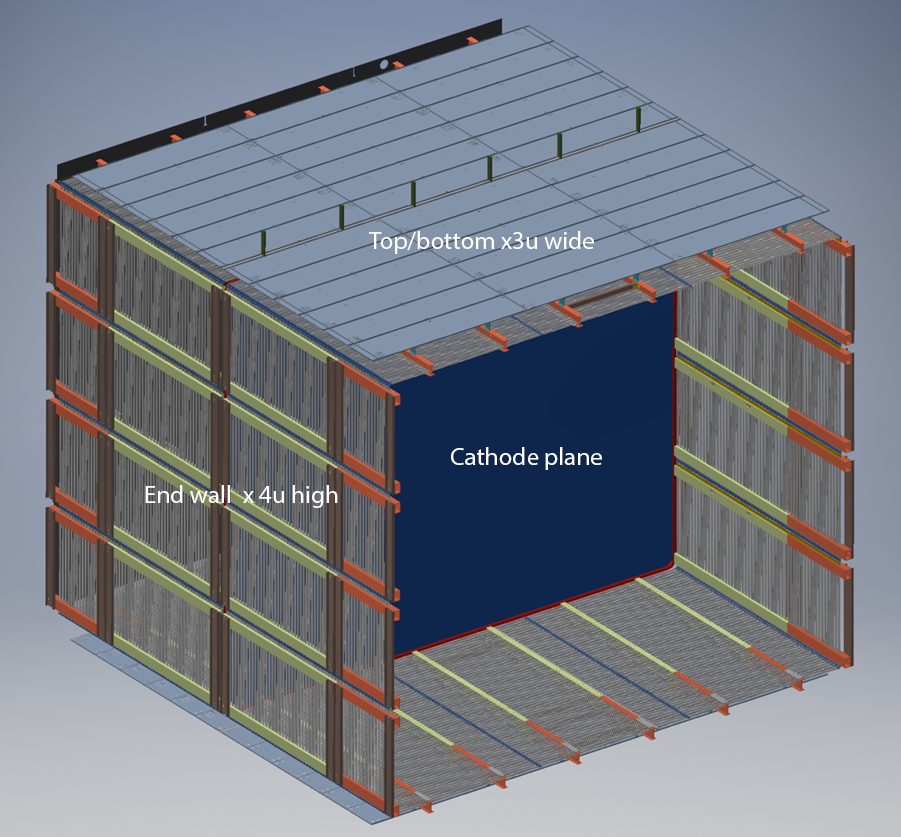
\includegraphics[width=0.6\linewidth]{tpc_fc_overview.png}
\end{cdrfigure}
\fixme{Figure~\ref{fig:fc-overview} needs a fuller, more descriptive caption}


\fixme{maybe need a bit of intro for the other components here, too}

%\chapter{det-comp}

%%%%%%%%%%%%%%%%%%%%%%%%%%%%%%%%%%%%%%%%%%%%%%
\section{Anode Plane Assemblies (APA)}

%%%%%%%%%%%%%%%%%%%%%%%%%%
\subsection{Scope and requirements}

Anode Plane Assemblies (APAs) are the detector elements utilized to sense ionization created by charged particles traversing the liquid argon volume inside the single-phase TPC.  The scope of the APAs includes:
\begin{itemize}
\item a framework of lightweight, rectangular stainless steel tubing;
\item a mesh layer attached directly to both sides of the APA frame;
\item layers of sense and shielding wires wrapped at varying angles relative to each other;
\item stacked head electronics boards, which are wire boards for anchoring the wires at the top (head) of the APA;
\item capacitive-resistive (CR) boards that link the wire boards to the CE;
\item side and foot boards along the other three edges of the APA with notches and pins to hold the wires in place;
%\item glue and solder;
\item modular boxes to hold the CE;
\item comb wire supports, mounted on cross braces distributed along the length of the APA, to prevent wire deflection; and
\item pin/slot pairs on the side edges of adjacent APAs to maintain coplanarity.
\end{itemize}

The initial physics performance requirements that drive the design of the APA are listed in Table~\ref{tab:physicsrequirements}.  These are chosen to enable high-efficiency reconstruction throughout the entire active volume of the LArTPC.  

\begin{cdrtable}[Prelim physics requirements that motivate APA design parameters]{lr}{physicsrequirements}{Preliminary physics requirements that motivate APA design parameters.}   
Requirement & Value  \\ \toprowrule
MIP Identification & 100$\%$ efficiency \\ \colhline
High efficiency for charge reconstruction & $>$90$\%$ for $>$100 MeV \\ \colhline
Vertex Resolution (x,y,z) & (1.5 cm, 1.5 cm, 1.5 cm)\\ \colhline
\textbf{Particle Identification} & \\ 
Muon Momentum Resolution & $<$18$\%$ for non-contained \\
            & $<$5$\%$ for contained\\ 
Muon Angular Resolution & $<$1$^{\circ}$\\            
Stopping Hadrons Energy Resolution & 1-5$\%$\\
Hadron Angular Resolution & $<$10$^{\circ}$ \\ \colhline
\textbf{Shower identification} & \\
Electron efficiency & $>$90$\%$\\
Photon mis-identification & $<$1$\%$\\
Electron Angular Resolution & $<$1$^{\circ}$ \\
Electron Energy Scale Uncertainty & $<$5$\%$\\
\end{cdrtable}

%\fixme{add drawing ahead of this table showing TPC coordinate system; per Justin}

The ability to identify minimum-ionizing particles (MIPs) is a function of several detector parameters, including argon purity, drift distance, diffusion, wire pitch, and Equivalent Noise Charge (ENC).  It is required that MIPs originating anywhere inside the active volume of the detector be reconstructed with 100$\%$ efficiency.   The choice of wire pitch (i.e., $\sim$5 mm), combined with the design values of the other high-level parameters, listed in Table~\ref{tab:apaparameters},  is expected to enable  this  efficiency.

The fine wire spacing of the APA enables excellent precision in identifying the location of any vertices in an event (e.g., the primary vertex in a neutrino interaction, or gamma conversion points in a $\pi^{0}$ decay), which has a direct impact on reconstruction efficiency. It is required to reach a vertex resolution of $\sim$1.5 cm along each coordinate direction.  In practice, the resolution on the drift-coordinate ($x$) of a vertex or hit will be better than that on its location in the $y$-$z$ plane, due to the combination of drift-velocity and electronics sampling-rate uncertainties.

%%%%%%%%%%%%%%%%
\subsection{APA design overview}
\label{sec:apa-design-overview}

An APA is constructed from a framework of lightweight, rectangular stainless steel tubing, with a fine mesh covering the rectangular area within the frame, on both sides, that defines a uniform ground across the frame. Along the length of the frame and around it, over the mesh layer, layers of sense and shielding wires are strung or wrapped at varying angles relative to each other, as illustrated in  Figure~\ref{fig:tpc_apa1}. The wires are terminated on  boards that anchor them and also provide the connections to the cold electronics. The APAs are 2.3\,m wide, 6.3\,m high, and 12\,cm thick.  
The size of the APAs is chosen for fabrication purposes, compatibility with over-the-road shipping, and for eventual transport to the 4850 level at SURF and installation into the membrane cryostat of a detector module. Sufficient shock absorption and clearances are taken into account at each stage.  The dimensions are also chosen such that an integral number of electronic readout channels and boards fill in the full area of the APA. The modularity of the APAs allows them to be built and tested at off-site production facilities, decoupling their manufacturing time from the construction of the membrane cryostat. 
As mentioned above, the principal design parameters are listed in Table~\ref{tab:apaparameters}.

\begin{cdrtable}[APA design parameters]{lr}{apaparameters}{APA design parameters}   
Parameter & Value  \\ \toprowrule
Active Height & 5.984 m\\ \colhline
Active Width & 2.300 m\\ \colhline
Wire Pitch (U,V) & 4.67 mm\\ \colhline
Wire Pitch (X,G) & 4.79 mm\\ \colhline
Wire Position Tolerance & 0.5 mm \\ \colhline
Wire Plane Spacing & 4.75 mm\\ \colhline
Wire Angle (w.r.t. vertical) (U,V) & 35.7$^{\circ}$\\ \colhline
Wire Angle (w.r.t. vertical) (X,G) & 0$^{\circ}$\\ \colhline
Number Wires / APA & 960 (X), 960 (G), 800 (U), 800 (V) \\ \colhline
Number Electronic Channels / APA & 2560 \\ \colhline
Wire Tension & 5.0 N \\ \colhline
Wire Material & Beryllium Copper \\ \colhline
Wire Diameter & 150 $\mu$m \\ \colhline
Wire Resistivity & 7.68 $\mu\Omega$-cm $@$ 20$^{\circ}$ C \\ \colhline
Wire Resistance/m & 4.4 $\Omega$/m $@$ 20$^{\circ}$ C \\ \colhline
Frame Planarity & 5 mm \\ \colhline
Photon Detector Slots & 10 \\
\end{cdrtable}


Starting from the outermost wire layer, 
there is first a shielding (grid) plane, followed by two induction planes, and finally the collection plane. All wire layers span the entire height of the APA frame. The layout of the wire layers is illustrated in  Figure~\ref{fig:tpc_apa1}.

\begin{cdrfigure}[APA diagram]{tpc_apa1}{Sketch of a ProtoDUNE-SP APA. This shows only portions of each of the three wire layers, U (green), V (magenta), the induction layers; and X (blue), the collection layer, to accentuate their angular relationships to the frame and to each other.  The induction layers are connected electrically across both sides of the APA.  The grid layer (G) wires (not shown), run vertically, parallel to the X layer wires;  separate sets of G and X wires are strung on the two sides of the APA.  The mesh is not shown.}
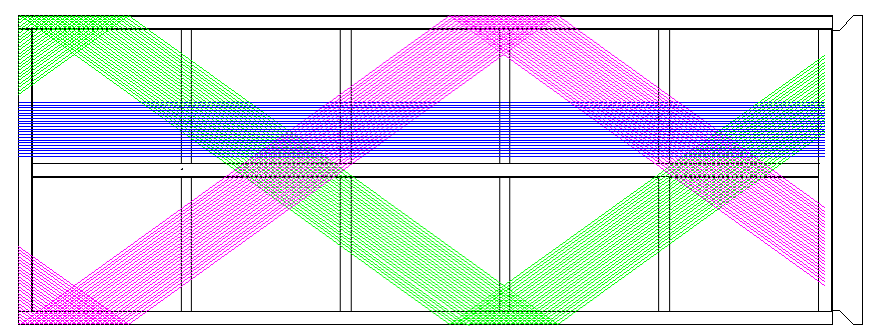
\includegraphics[width=0.8\textwidth, angle=90]{figures/tpc_apa1.png} 
\end{cdrfigure}

The angle of the induction planes in the APA ($\pm$35.7$^{\circ}$) is chosen such that each induction wire only crosses a given collection wire one time, reducing the ambiguities that the reconstruction must address.  The design angle of the induction wires, coupled with their pitch, was also chosen such that an integer multiple of electronics boards reads out one APA.

The wires of the grid (shielding) layer, G,  are not connected to the electronic readout; the wires run parallel to the long edge of the APA frame; there are separate sets of G wires on the two sides of the APA. 
 The two planes of induction wires (U and V) wrap in a helical fashion around the long edge of the APA, continuously around both sides of the APA.  The collection plane wires (X) run vertically, parallel to G.   The ordering of the layers, from the outside in, is G-U-V-X, followed by the mesh.   

The operating voltages of the APA layers are listed in Table~\ref{tab:bias}.  When operated at these voltages, the drifting ionization follows trajectories around the grid and induction wires, ultimately terminating on a collection plane wire; i.e., the grid and induction layers are completely transparent to drifting ionization, and the collection plane is completely opaque.  The grid layer is present for pulse-shaping purposes, effectively shielding the first induction plane from the drifting charge and removing the long leading edge from the signals on that layer; again, it is not connected to the electronics readout. The mesh layer serves to shield the sense planes from pickup from the Photon Detection System and from ``ghost'' tracks that would otherwise be visible when ionizing particles have a trajectory that passes through the collection plane. 

\begin{cdrtable}[Baseline bias voltages for APA wire layers]{lr}{bias}{Baseline bias voltages for APA wire layers}   
Anode Plane & Bias Voltage  \\ \toprowrule
Grid (G) & -665 V\\ \colhline
Induction (U) & -370 V\\ \colhline
Induction (V) & 0 V\\ \colhline
Collection (X) & 820 V\\ \colhline
Mesh (M) & 0 V\\
\end{cdrtable}

The wrapped style allows the APA plane to fully cover the active area of the LArTPC, minimizing the amount of dead space between the APAs that would otherwise be occupied by electronics and associated cabling.   

In the current design of the DUNE-SP far detector module, a central row of APAs is flanked by  drift-fields, requiring sensitivity on both sides. The wrapped APAs allow the induction plane wires to sense drifting ionization originating from either side of the APA.  This double-sided feature is not strictly necessary for the ProtoDUNE-SP arrangement, which has APAs located against the cryostat walls and a drift field on one side only, but it is compatible with this setup as the grid layer facing the wall effectively blocks any ionization generated outside the TPC from drifting in to the wires on that side of the APA.

The choices of wire tension and wire placement accuracy are made to ensure proper operation of the LArTPC at voltage, and to provide the precision necessary for reconstruction.  The tension of 5~N, when combined with the intermediate support combs (described in Section~\ref{subsec:apa_combs}) ensure that the wires are held taught in place with no sag.  Wire sag can impact the precision of reconstruction, as well as the transparency of the TPC.  The tension of 5~N is low enough that when the wires are cooled, which increases their tension due to thermal contraction, they will stay safely below the break load of the beryllium copper wire, as described in Section~\ref{subsec:apa_wires}.  To further mitigate wire breakage and its impact on detector performance, each wire in the APA is anchored twice on both ends, with both solder and epoxy.  %Details of this arrangement are provided in Section~\ref{subsubsec:apa_wire_wrap}. 


%%%%%%%%%%%%
\subsection{Wire properties}
\label{subsec:apa_wires}

Beryllium copper (CuBe) wire is known for its high durability and yield strength. It is composed of $\sim$98$\%$ copper, 1.9$\%$ beryllium, and a negligible amount of other elements. The APA wire has a diameter of 150$\mu$m (.006~in), and is strung in varying lengths across the APA frame. Three key properties for its usage in the APA are: low resistivity, high tensile or yield strength, and coefficient of thermal expansion suitable for use with the APA's stainless steel frame.

Tensile strength of the wire describes the wire-breaking stress (see Table~\ref{tab:wire}).  The yield strength is the stress at which the wire starts to take a permanent (inelastic) deformation, and is the important limit stress for this case, though most specifications give tensile strength.  Fortunately, for the CuBe alloys of interest, the two are fairly close to each other.  Based on the tensile strength of wire purchased from Little Falls Alloy (over 1,380~MPa or 200,000~psi), the yield strength is greater than 1,100~MPa.  Given that the stress while in use is around 280~MPa, this leaves a comfortable margin.

The coefficient of thermal expansion (CTE) describes how material expands and contracts with changes in temperature.  The CTEs of CuBe alloy and 304 stainless steel are very similar.  Integrated down to 87~K, they are 2.7e-3 for stainless and 2.9e-3 for CuBe~\cite{cryo-mat-db}.
Since the wire contracts slightly more than the frame during cool-down the wire tension increases.  If it starts at 5~N, the tension rises to about 5.5~N when everything is cool.  

The change in wire tension during cool-down could also be a concern.  In the worst case, the wire
 cools quickly to 87\,K before any significant cooling of the frame  -- a realistic case because of the differing thicknesses.  In the limiting case, with complete contraction of the wire and none in the frame, the tension would be expected to reach $\sim$11.7 N.  This is still well under the $\sim$20 N yield tension.
In practice, the cooling will be done gradually to avoid this tension spike as well as other thermal shock to the APA.

\begin{cdrtable}[CuBe wire tensile strength and CTE]{lr}{wire}{Tensile strength and coefficient of thermal expansion (CTE) of beryllium copper (CuBe) wire.}
%\multicolumn{2}{c}{Properties of beryllium copper wire} \\ 
Parameter & Value \\ \toprowrule
Tensile Strength (from property sheets) (psi) & 208,274 \\ \colhline
Tensile Strength (from actual wire) (psi) & 212,530 \\ \colhline
CTE of CuBe, integrated to 87 K (m/m) & 2.9e-3 \\ \colhline
CTE of 304 stainless steel, integrated to 87 K (m/m) & 2.7e-3 \\
\end{cdrtable}


%%%%%%%%%%%%
\subsection{APA frame and mesh}
\label{subsec:apa_frame}

%\paragraph{Dimensions}

The stainless steel frame of the APA (Figure~\ref{fig:tpc_apa_frame}) is 6.06~m long, not counting electronics and mounting hardware, and 2.30~m wide.  It is 76.2~mm thick, made from imperial size 3-in $\times$ 4-in $\times$ 0.120-in wall rectangular tubing.  The cross pieces have a cross-sectional area of 2\,in $\times$ 3\,in, and are connected to edge pieces using joints, as in Figure~\ref{fig:tpc_apa_boltedjointdrawing}.  It is mounted in the cryostat with its long axis vertical; multiple APAs are mounted edge-to-edge to form a continuous plane. An electron deflection technique, described in Section~\ref{sec:apa:electrondiverter}, is used to ensure that electrons drawn towards a joint between two APAs will be deflected to one or the other, and not lost.

\begin{cdrfigure}[APA dimensions]{tpc_apa_frame}{An APA showing overall dimensions and main components. }
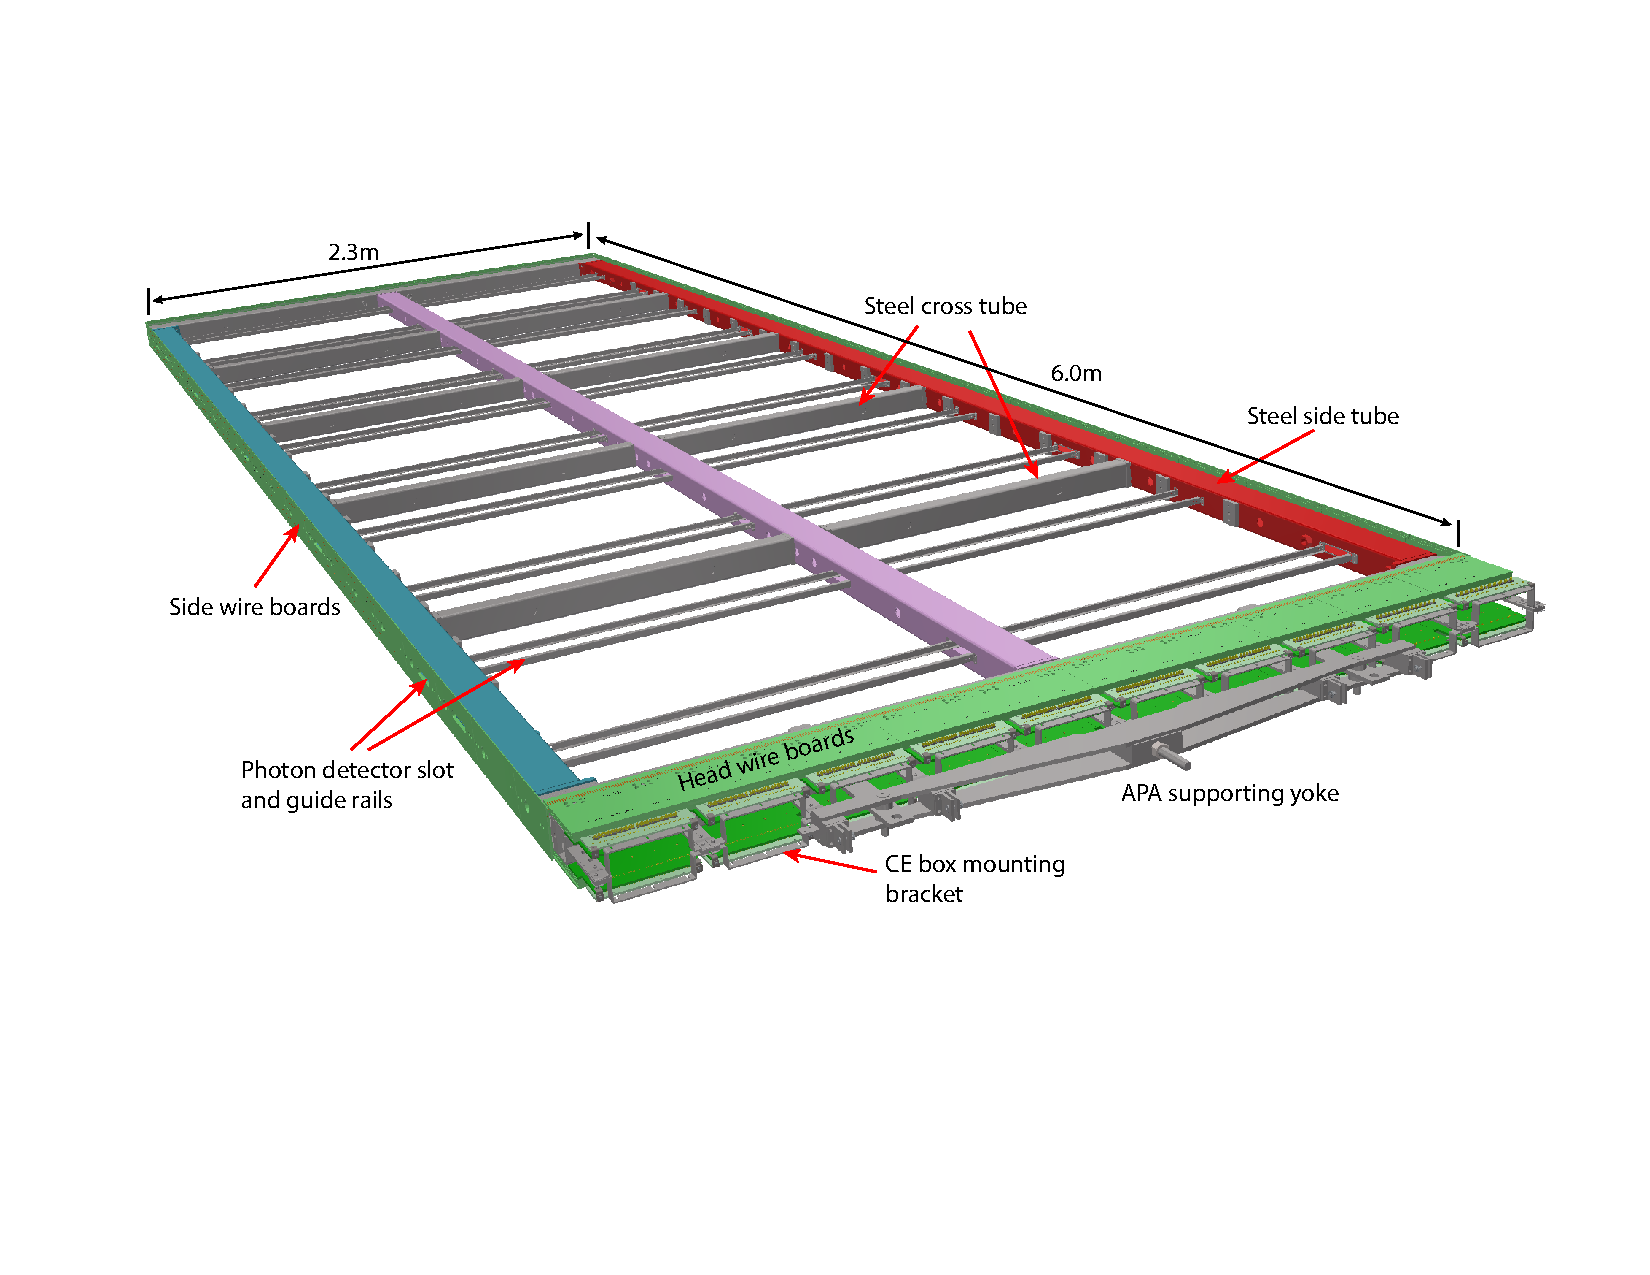
\includegraphics[width=0.9\textwidth]{figures/tpc_apa_frame} 
\end{cdrfigure}
%\fixme{COMMENT from Justin: it would be good if the dimensions of the upper figure had the same precision as the numbers in the text, i.e. 6.06 m and 2.30 m. (Anne agrees, but we're not updating figures right now.)}

\begin{cdrfigure}[APA bolted joint drawing]{tpc_apa_boltedjointdrawing}{A model of the bolted joint.  The holes on the top of the tube are for access to tighten the screws.  The heads actually tighten against the lower hole, inside the tube.}
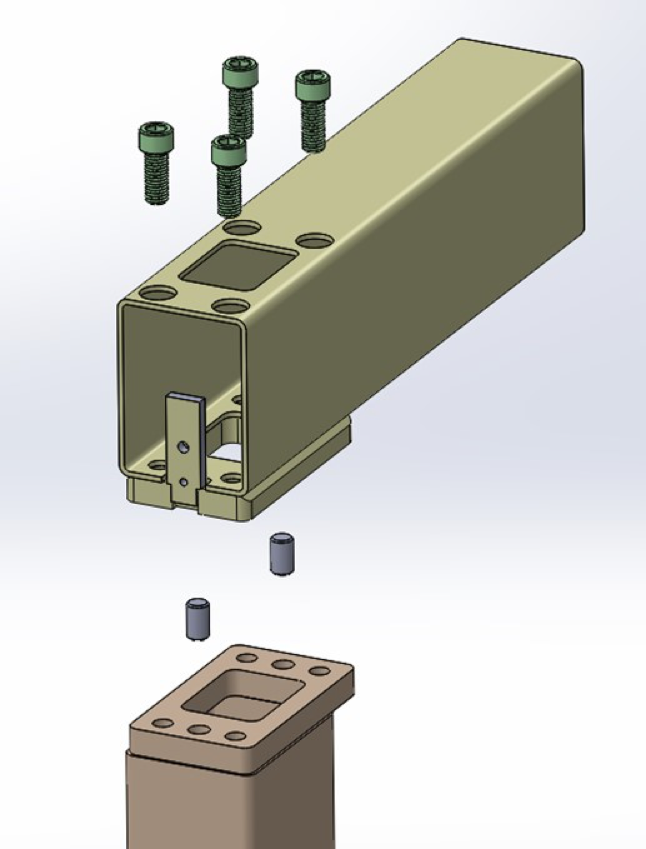
\includegraphics[width=0.4\textwidth]{figures/tpc_apa_boltedjointdrawing.png} 
\end{cdrfigure}

A fine mesh screen is glued directly to the steel frame surface, over the frame on both sides.  It creates a uniform ground layer beneath the wire planes.  

The mesh is clamped around the perimeter of the opening and then pulled tight (by opening and closing clamps as needed during the process).  When the mesh is taut, a 25-mm-wide strip is masked off around the opening and glue is applied through the mesh to attach it to the steel.  Although measurements have shown that this gives good electrical contact between the mesh and the frame, a deliberate electrical connection is also made.  Figure~\ref{fig:tpc_apa_fullsizemeshdrawing} depicts the mesh application setup for a full-size ProtoDUNE-SP APA.

\begin{cdrfigure}[APA full-size mesh drawing]{tpc_apa_fullsizemeshdrawing}{The mesh clamping jig for the full size APA. }
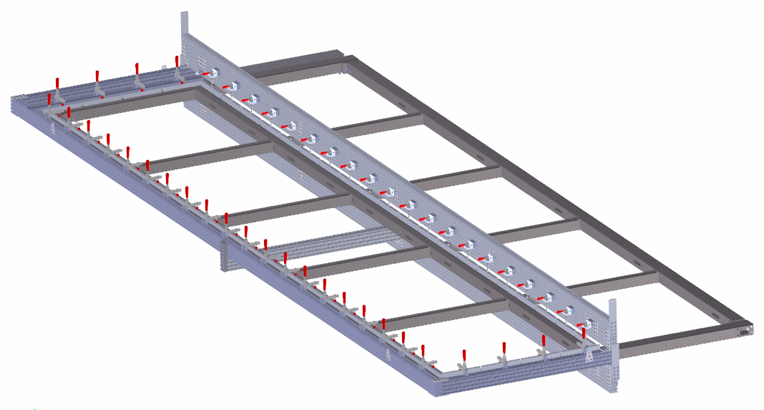
\includegraphics[width=0.8\textwidth]{figures/tpc_apa_fullsizemeshdrawing.png} 
\end{cdrfigure}


%%%%%%%%%%%%%%%%%%%%%%%%
\subsection{Anchoring elements and wire boards}
\label{subsubsec:apa_wire_anchor}


%%%%%%%%%%%%
\subsubsection{Head electronics boards}

At the head end of the APA, stacks of electronics boards (referred to as ``wire boards'') are arrayed to anchor the wires.  They also provide the connection between the wires and the %data acquisition electronics -- usually called the 
cold electronics.

All APA wires are terminated on the wire boards, which are stacked along the electronics end of the APA frame; see Figure~\ref{fig:tpc_apa_boardstack}. 
Attachment of the wire boards begins with the X plane (innermost). After the X-plane wires are strung top to bottom along each side of the APA frame, they are soldered and epoxied to their wire boards and trimmed. The remaining wire board layers are attached as each layer is wound.  The main CR boards (capacitive-resistive), which provide DC bias and AC coupling to the wires, are attached to the bottom of the wire board stack. %They are described here.

\begin{cdrfigure}[APA board stack]{tpc_apa_boardstack}{Left: View of the APA wire board stack, as seen from the top/side. The wire board layers can be seen at the bottom-left of the illustration, X on the bottom (it doesn't go all the way back, but extends farther forward and has the main CR board attached), followed by U, V, then G (which doesn't go all the way forward, and has its own CR board attached). Right: the same stack viewed from below. }
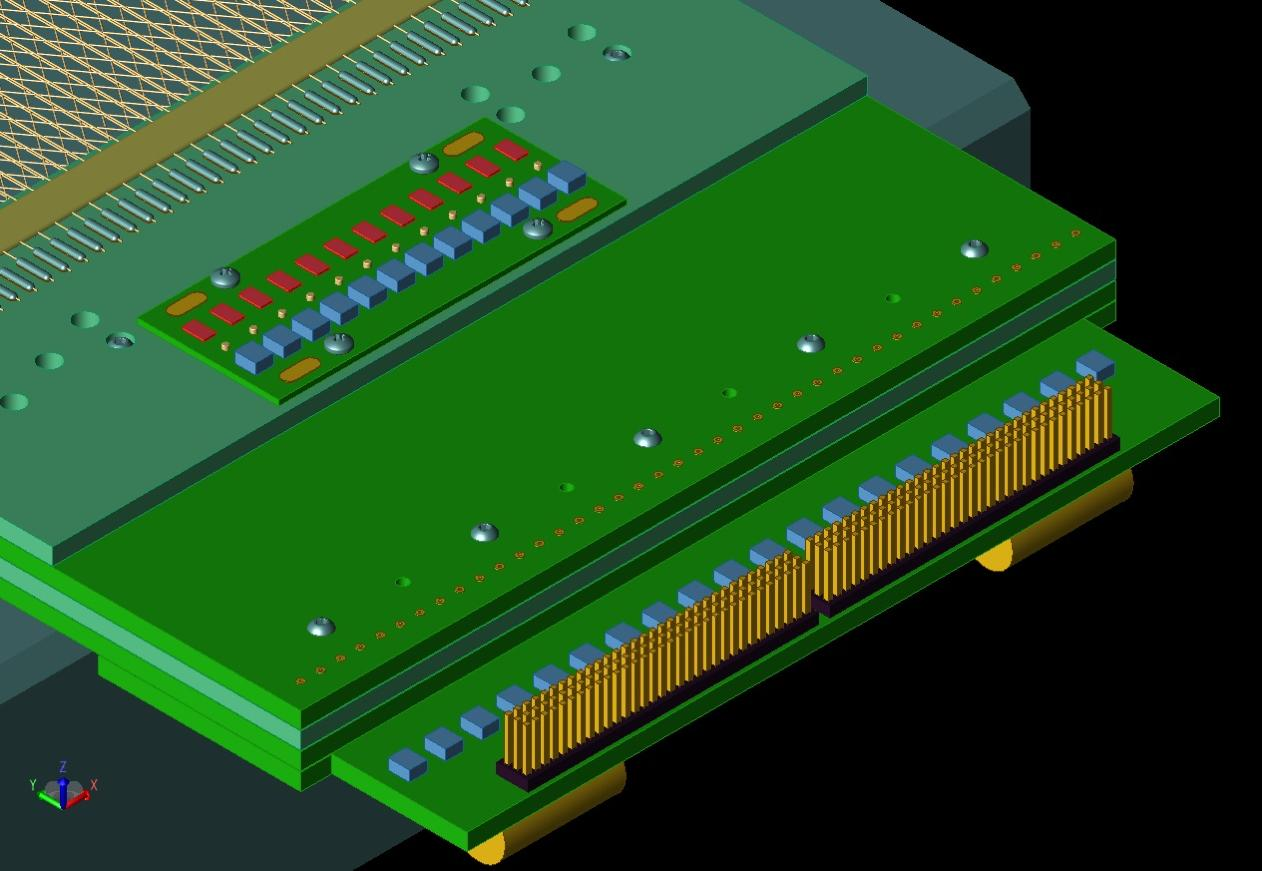
\includegraphics[width=0.45\textwidth]{figures/tpc_apa_boardstack_top}
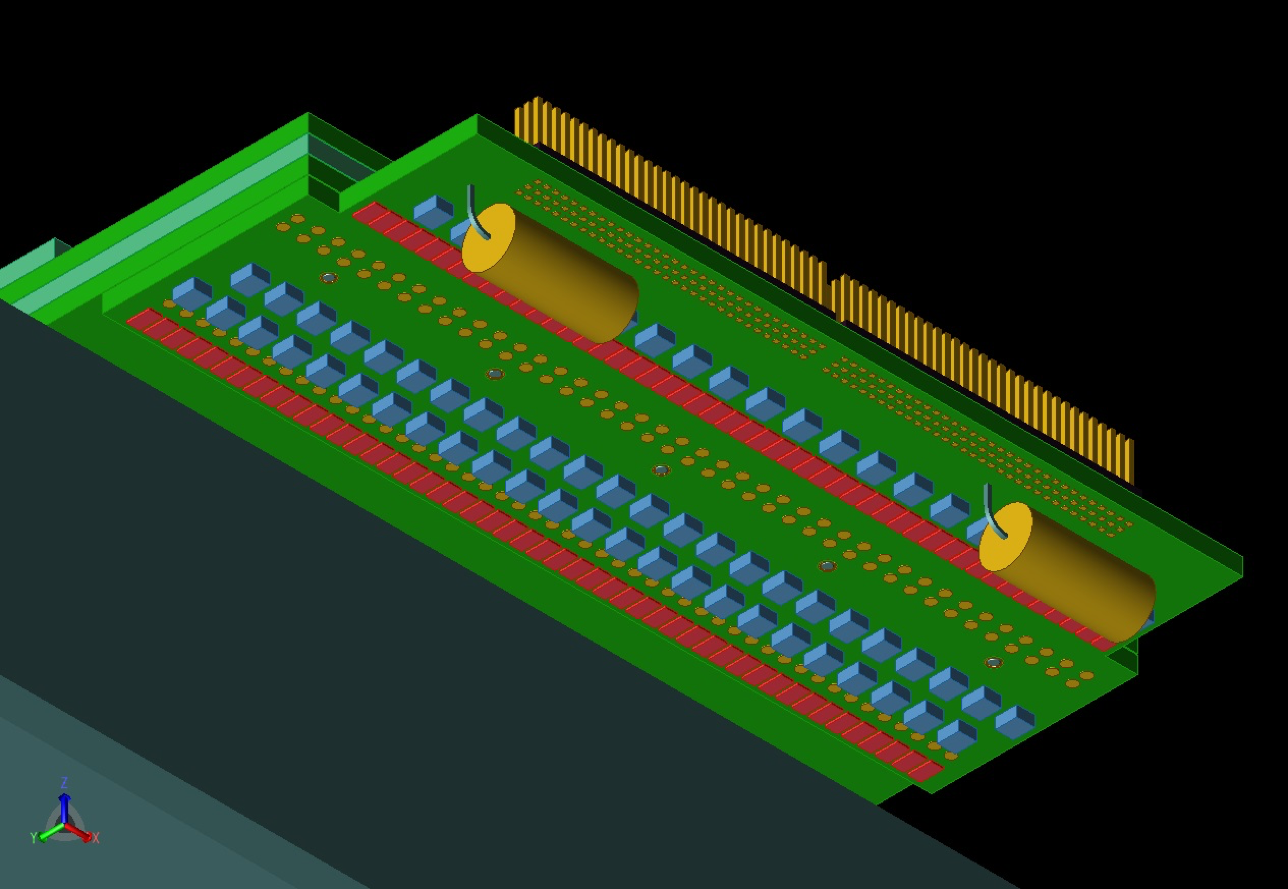
\includegraphics[width=0.45\textwidth]{figures/tpc_apa_boardstack_bottom}
\end{cdrfigure}

%\fixme{figure \ref{fig:tpc_apa_boardstack} needs labeling}

The outermost G-plane wire boards connect adjacent groups of four wires together, and bias each group through an R-C filter whose components are placed on special CR boards  %The filter components are located on daughter boards 
that are attached after the wire plane is strung. The X, U and V layers of wires are connected to the CE (housed in boxes mounted on the APA) either directly or through DC-blocking capacitors. The X and U planes have wires individually biased through 50-M$\Omega$ resistors. Electronic components for the X- and U-plane wires are located on a common CR board. 

Mill-Max pins and sockets provide electrical connections between circuit boards within a stack. They are pressed into the circuit boards and are not repairable if damaged. To minimize the possibility of damaged pins, the boards are designed so that the first wire board attached to the frame has only sockets. All boards attached subsequently contain pins that plug into previously mounted boards. This process eliminates exposure of any pins to possible damage during winding, soldering, or trimming processes.

Ten stacks of wire boards are installed across the width of each side along the head of the APA.  The X-layer board in each stack has room for 48 wires, the V layer has 40 wires, the U layer 40 wires and the G layer 48 wires.  Each board stack, therefore, has 176 wires but only 128 signal channels since the G wires are not read out.  
With a total of 20 stacks per APA, this results in 2,560 signal channels per APA and a total of \SI{3520} wires starting at the top of the APA and ending at the bottom.  There is a total of $\sim$23.4 km of wire on the two surfaces of each APA.  Many of the capacitors and resistors that in principle could be on these wire boards are instead
placed on the attached CR boards to improve their accessibility in case of component failure.   Figure~\ref{fig:tpc_apa_electronics_connectiondiagram} depicts the connections between the different elements of the APA electrical circuit. %\fixme{this figure could use some labelling}

At the head end of the APA, the wire-plane spacing is set by the thickness of these wire boards.  The first layer's wires solder to the surface of the first board, the second layer's wires to the surface of the second board, and so on.  For installation, temporary toothed-edge boards beyond these wire boards align and hold the wires until they are soldered to pads on the wire boards.  After soldering, the extra wire is snipped off. 

\begin{cdrfigure}[APA wire board connection to electronics]{tpc_apa_electronics_connectiondiagram}{Diagram of the connection between the APA wires, viewed from the APA edge. The set of wire boards within a stack can be seen on both sides of the APA, with the CR board extending further to the right, providing a connection to the cold electronics, which are housed in the boxes at the far right of the figure. }
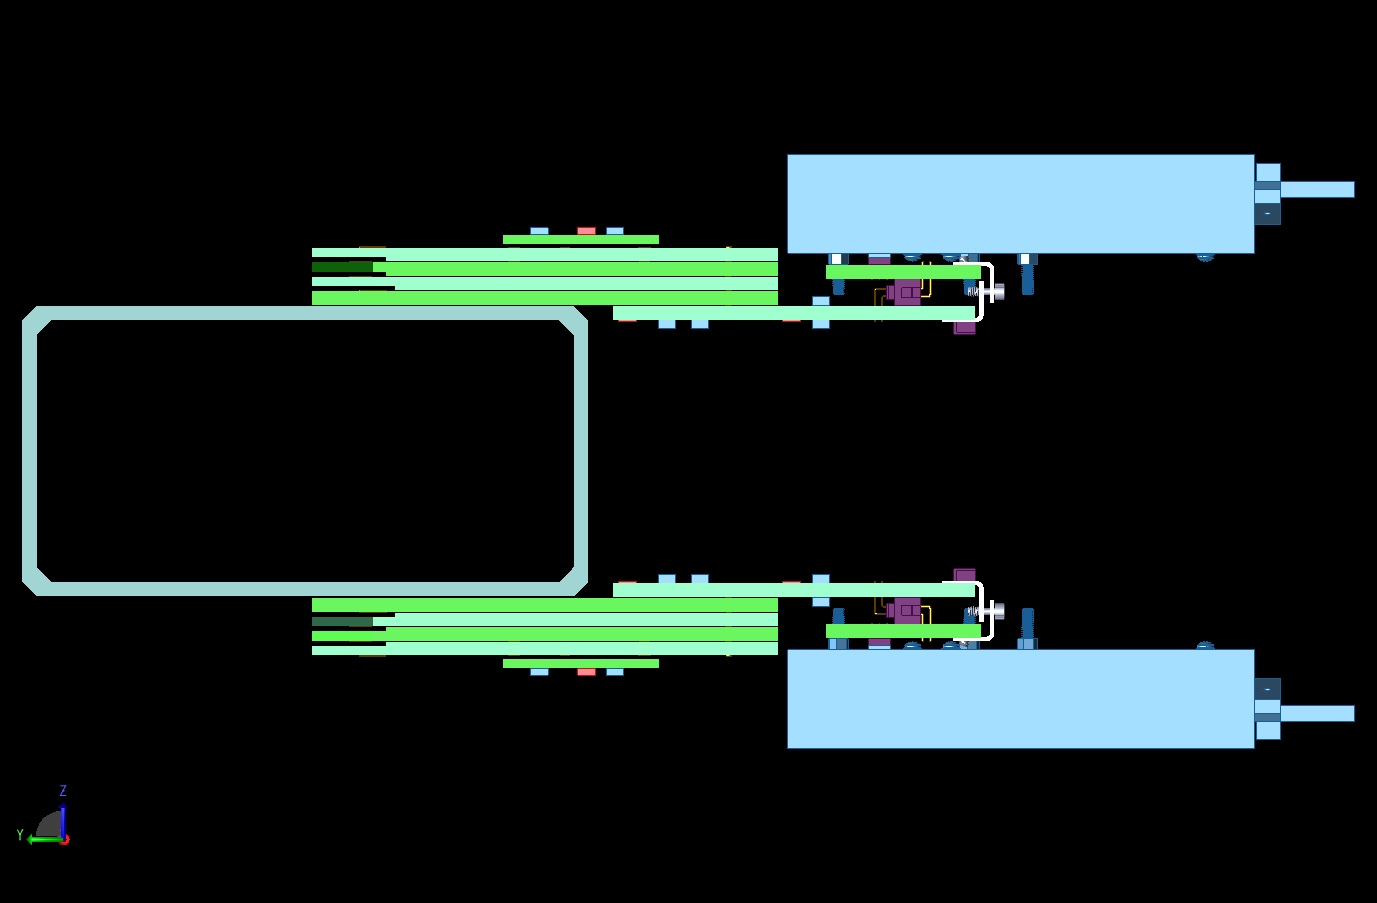
\includegraphics[width=0.7\textwidth]{figures/tpc_apa_electronics_connectiondiagram}
\end{cdrfigure}

%%%%%%%%%%%%
\subsubsection{CR boards}
\label{sec:crboards}

The CR boards carry a bias resistor and a DC-blocking capacitor for each wire in the X and U planes. These boards are attached to the board stacks after fabrication of all wire planes.  Electrical connections to the board stack are made though Mill-Max pins that plug into the wire boards. Connections from the CR boards to the CE are made through a pair of 96-pin Samtec connectors.

Surface-mount bias resistors on the CR boards have resistance of 50\,M$\Omega$ are constructed with a thick film on a ceramic substrate. Rated for 2.0-kV operation, the resistors measure 0.12 $\times$ 0.24 inches. Other ratings include operation from $-$55 to +155 C, 5\% tolerance, and a 100-ppm/C temperature coefficient.
Performance of these resistors at LAr temperature is verified through additional bench testing.

The selected DC-blocking capacitors have capacitance of 3.9\,nF and are rated for 2.0-kV operation. Measuring 0.22 $\times$ 0.25\,inches across and 0.10\,inches high, the capacitors feature flexible terminals to comply with PC board expansion and contraction. They are designed to withstand 1,000 thermal cycles  
between the extremes of the operating temperature range. Tolerance is also 5\%.

%\fixme{Eric has question mark on the temp range}

In addition to the bias and DC-blocking capacitors for all X- and U-plane wires, the CR board includes two R-C filters for the bias voltages. The resistors are of the same type used for wire biasing except with a resistance of 2\,M$\Omega$. Capacitors are 47\,nF at 2\,kV. Very few choices exist for surface-mount capacitors of this type, and they are exceptionally large. %Currently the plan is to use 
Polyester or Polypropylene film capacitors that are known to perform well at cryogenic temperatures are used.


%%%%%%%%%%%%
\subsubsection{Side and foot boards}

The boards along the sides and foot of the APA have notches, pins and other location features to hold the wires in the correct position as they wrap around the edge from one side of the APA to the other.

G10 circuit board material is ideal for these side and foot boards due to its physical properties alone, but it has an additional advantage: a number of hole or slot features in the edge boards provide access to the underlying frame.  In order that these openings are not covered by wires, the sections of wire that would go over the openings are replaced by traces on the boards.  After the wires are wrapped, the wires over the opening are soldered to pads at the ends of the traces, and the section of wire between the pads is snipped out (Figure~\ref{fig:tpc_apa_sideboardmodel}).  These traces are easily and economically added to the boards by the many commercial fabricators who make circuit boards. 

\begin{cdrfigure}[APA side board model]{tpc_apa_sideboardmodel}{Model of board with wires showing how traces connect wires around openings in the side boards.  The wires are wound straight over the openings, then soldered to pads at the ends of the traces.  After soldering the sections between the pads are trimmed away.}
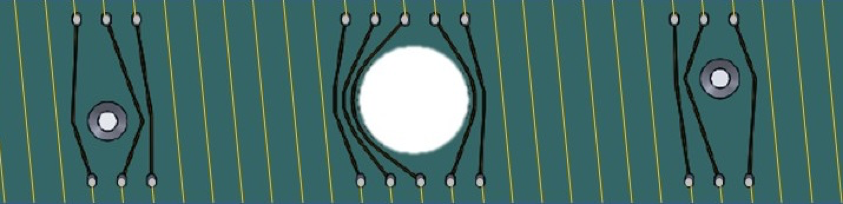
\includegraphics[width=0.9\textwidth]{figures/tpc_apa_sideboardmodel.png} 
\end{cdrfigure}


\begin{cdrfigure}[APA side board photo]{tpc_apa_sideboardphoto}{Boards with injection molded tooth strips glued on.  The left shows an end board with teeth for fixing the position of the longitudinal wires.  The teeth there form small notches. The right is a side board for fixing the position of the angled wires where the wires are angled around a pin. (These boards are prototype test pieces and are not used in the production APAs.)}
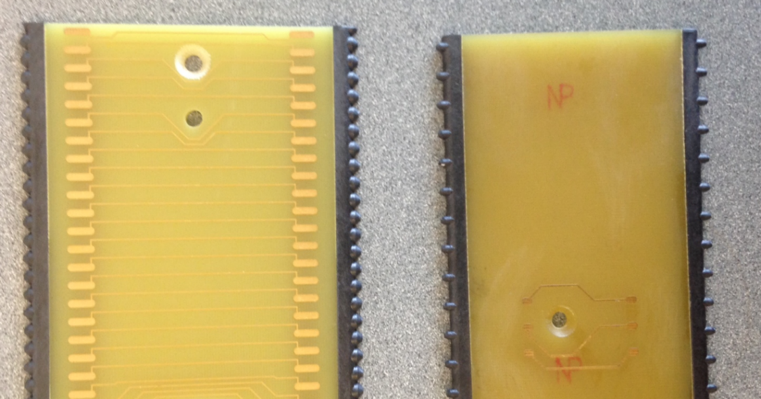
\includegraphics[width=0.7\textwidth]{figures/tpc_apa_sideboardphoto.png} 
\end{cdrfigure}

The placement of the angled wires are fixed by pins 
as shown in the right-hand picture of Figure~\ref{fig:tpc_apa_sideboardphoto}.  The wires make a partial wrap around the pin as they change direction from the face of the APA to the edge.  The X- and G-plane wires are not pulled to the side so they cannot be pulled against a pin.  Their positions are fixed %located 
by teeth with slots, as shown in the left-hand picture in Figure~\ref{fig:tpc_apa_sideboardphoto}. 
	
The polymer used for the strips is Vectra e130i (a trade name for 30$\%$ glass filled liquid crystal polymer or LCP). It retains its strength at cryogenic temperature and has a CTE similar enough to G10 that differential expansion/contraction is not a problem.

%%%%%%%%%%%%
\subsubsection{Glue and solder}
The ends of the wires are soldered to pads on the edges of the wire boards.  Solder provides both an electrical connection and a physical anchor to the wires.  As an additional physical anchor, roughly 10~mm of the wires are glued near the solder pads.  For example, in Figure~\ref{fig:tpc_apa_sideboardphoto}, in addition to soldering the wires on the pads shown in the left-hand photograph, an epoxy bead is applied on the wires in the area between the solder pads and the injection-molded tooth strips.

Gray epoxy 2216 by 3M is used for the glue.  It is strong, widely used (therefore much data is available), and it retains good properties at cryogenic temperatures.  A 62$\%$ tin, 36$\%$ lead and 2$\%$ silver solder was chosen.  A eutectic mix (63/37) is the best of the straight tin/lead solders but the 2$\%$ added silver gives better creep resistance.

%%%%%%%%%%%%
\subsubsection{Comb wire supports on inner frame members}
\label{subsec:apa_combs}

%\paragraph{Purpose}

Some wire segments are quite long; for instance, the X- and G-plane wires 
extend from one end of the APA to the other without going around a side -- a length of 6\,m.  Even the diagonal wires across the middle of the APA are 3.9\,m long.  To prevent deflection from gravity, electrostatic forces, or liquid drag from moving argon, the wires are supported at regular locations along the length of the APA.  This is done with \textit{combs} mounted on each of the four cross braces that are  %evenly 
regularly spaced along the length of the APA.  This keeps the longest unsupported wire length under 1.6\,m.

The nominal wire tension is 5\,N but even the 1.6-m-long wires could fall to 3\,N of tension before the wire, held horizontally, would deviate 150\,microns -- one wire diameter.  During operation the wires are either vertical or 35.7$^{\circ}$ from vertical, so the actual deviation would be less.

%\paragraph{Geometry}

The combs are made from 0.5-mm-thick G10 with slots cut into it.  The comb for the lowest layer is glued to a base strip that is glued to the frame.  After each layer is wound, another comb strip is glued to the tips of the teeth of the previous one to position the wires in the next layer.  Each successive comb holds the previous layer of wires in the bottom of its slots (Figure~\ref{fig:tpc_apa_supportcombmodel}).

\begin{cdrfigure}[APA support comb model]{tpc_apa_supportcombmodel}{A model of the combs showing how they stack.  After winding a layer, the comb for the next layer is put in place.  Each comb holds the wires from the previous layer in its slots.}
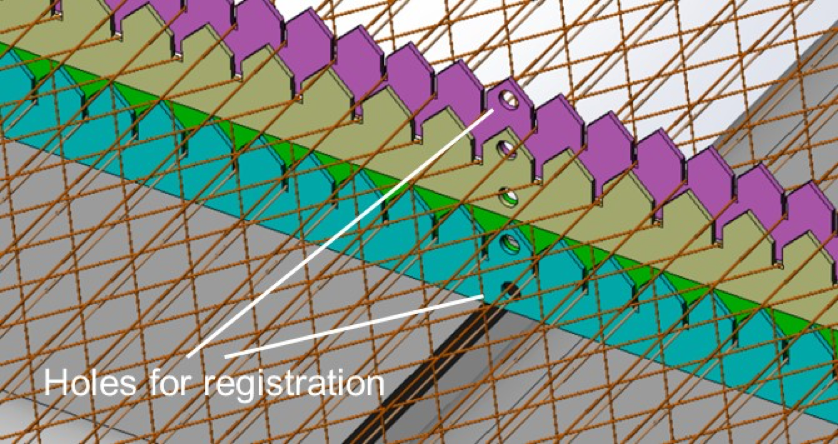
\includegraphics[width=0.7\textwidth]{figures/tpc_apa_supportcombmodel.png} 
\end{cdrfigure}

Periodic holes along the length of the strip allow the use of pins to accurately position each successive strip with respect to the previous one.  A series of jigs is used to create and install these combs.  One jig aligns the first strip to the base strip during gluing.  Another jig locates this assembly on the frame as it is glued in place. A third jig locates each successive comb using these holes (labeled registration holes in Figure~\ref{fig:tpc_apa_supportcombmodel}).

The wire openings in the comb stack are small enough that the wires are accurately positioned at the combs, and therefore the gluing of wires into the combs is not required.

%%%%%%%%%%
\subsubsection{Electron diverter}
\label{sec:apa:electrondiverter}
 
The active aperture of the collecting plane wires is 2300\,mm wide, while the APA modules are installed at a 2320\,mm pitch.  This leaves a 20\,mm gap between two adjacent APAs that is occupied by the stacks of wire wrapping boards and some clearance space. Electrons from the ionizing tracks drifting over the gap have an ill-defined trajectory; some get lost and some land on the wrong wire and create unexpected signal waveforms.  A set of \textit{electron diverters} installed between APAs would nudge the incoming electrons away from the gap, towards %a wire in the active aperture. 
an active collection wire. It is planned to install electron diverters between some of the ProtoDUNE-SP APAs to determine whether they should be included in the DUNE-SP detector design.
 
The electron diverter is a set of thin printed circuit boards with two strip electrodes sticking up from the first wire plane.  The two electrodes are biased at %more 
negative voltages with respect to to the natural potential at their locations.  A repulsive force from these electrodes pushes the incoming electrons away %so they do not land in 
from the inactive gap.  Figure~\ref{fig:tpc_apa_e_diverter} illustrates the principle. The left plot shows the E-field lines near the symmetry plane between two APAs, where a roughly 10-mm band of field lines land on the edge of the boards holding the wrapped wires.  The right plot shows the field lines with the electron diverter installed (at the left edge of the plot); here, all field lines are pushed to the active region.

\begin{cdrfigure}[Field maps of the region near the inactive gap of an APA]{tpc_apa_e_diverter}{Left: field map of the region near the inactive gap of an APA without the electron diverter; Right: field map with the electron diverter in place.
Electric field lines are shown in black, equipotential contours are in white, and electric field strength is represented in color gradient.}
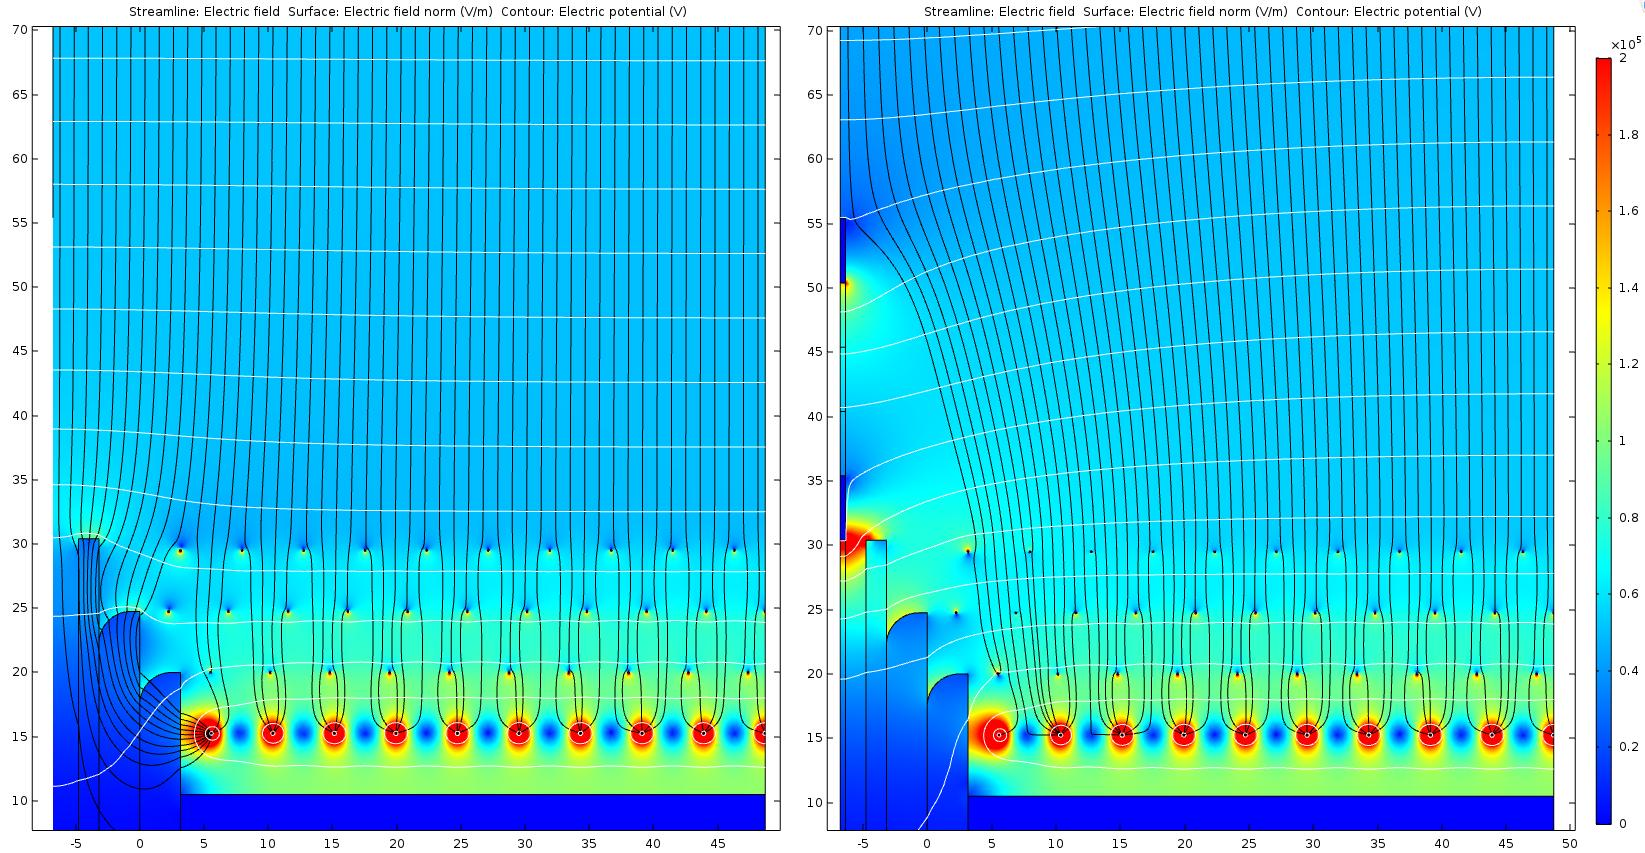
\includegraphics[width=0.9\textwidth]{tpc_apa_e_diverter} 
\end{cdrfigure}

 
The leading edge of the diverter board is 25\,mm above the grid plane.  The first electrode is flush with the leading edge of the board, and the second electrode just clears the grid plane.  Both of them are 5\,mm wide.  The leading electrode is biased at a nominal voltage of $-$2300\,V, and the inner is biased at -1300\,V.     Figure\ref{fig:tpc_apa_e_diverter_on_apa} shows the electron diverter boards mounted on a side of an APA.  A total of 10 boards are screwed onto the APA frame using existing tapped holes.  The topmost board has low pass RC network to filter the voltages fed to the electrodes.  These boards will be installed on two APAs on one side of the drift, leaving the other drift volume without such a feature, for comparison.
 
 \begin{cdrfigure}[Corner of APA with electron diverter boards installed]{tpc_apa_e_diverter_on_apa}{A view of a corner of an APA with a full set of electron diverter boards installed (along right-hand edge in diagram).  The first board, with its end at the top of the APA (the top of the APA is in the foreground) has the bias voltage connectors and RC filtering network (brown with blue connectors protruding).  The reddish-brown strips on the boards are the strip electrodes. The rest of the boards (delineated by blue lines) are interconnected %to the first boards 
 through copper wires soldered to the ends of the strip electrodes.}
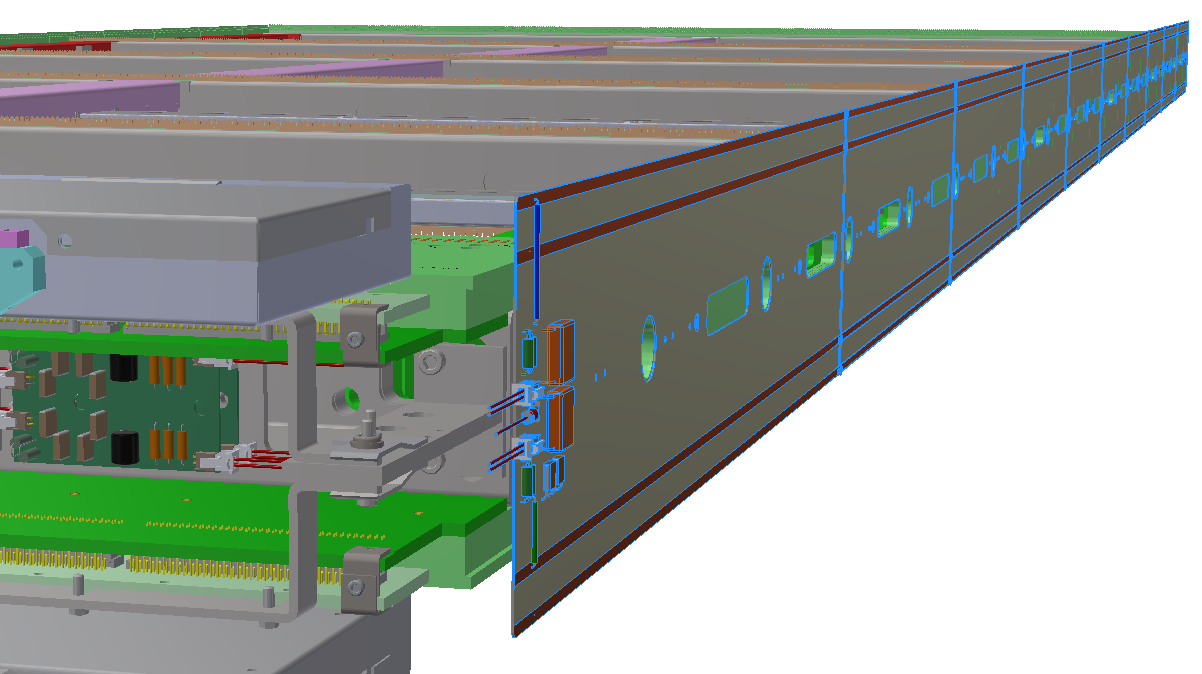
\includegraphics[width=0.9\textwidth]{tpc_apa_e_diverter_on_apa} 
\end{cdrfigure}


%%%%%%%%%%%%
\subsection{Interconnection features}

%%%%%%%%%%%%
\subsubsection{CE boxes}

Pins extending outward from the CR boards provide connections from the APA to the modularly designed CE, and the CE modules are housed in small boxes that provide shielding.
The CE boxes are illustrated in Figure~\ref{fig:tpc_apa_electronicsmountingdiagram}. 
%The design being developed for attaching the CE to the APAs consists of small boxes, 
Each board stack has one CE box installed near it that holds the CE module for the stack.  

Putting the electronics in small boxes simplifies installation and replacement, and also helps with the dissipation 
%\fixme{getting rid of}
of argon gas generated by the warm electronic components.  The CE modules are mounted in such a way that any of them can be removed from a single side of the APA after APA installation.

\begin{cdrfigure}[Solid model of modular CE boxes]{tpc_apa_electronicsmountingdiagram}{Solid model of %revised, 
modular CE boxes.}
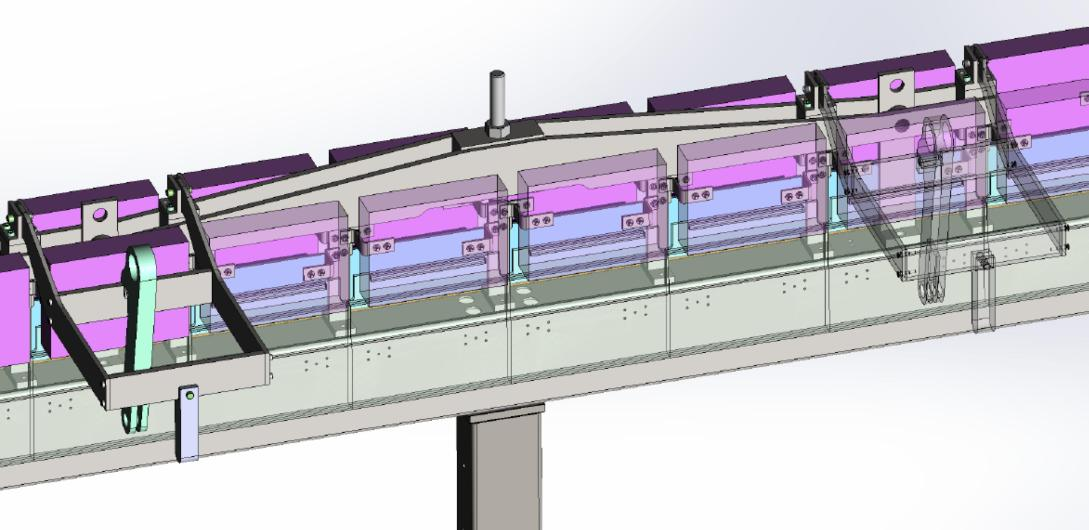
\includegraphics[width=0.9\textwidth]{figures/tpc_apa_electronicsmountingdiagram.png} 
\end{cdrfigure}

%%%%%%%%%%%%
\subsubsection{Adjacent APAs}

A constraint is needed between adjacent APAs to keep them co-planar.  It is also important that this constraint not apply a vertical load to adjacent APAs.  The constraint takes the form of 
 a pair of protruding pins on one edge of the APA (one high and one low) and a pair of matching slots %on the other edge 
on the edge of the adjacent APA
to engage the pins (Figure~\ref{fig:tpc_apa_pinslotdrawing}). The pins have steel cores for strength.

\begin{cdrfigure}[APA interconnect drawing]{tpc_apa_pinslotdrawing}{The pin/slot constraint.  The pin screws into an insert in the outside frame member of one APA and engages a slot in the outside frame member of the adjacent APA. An insulating sleeve surrounds the guiding pin to ensure electrical isolation between the APAs.}
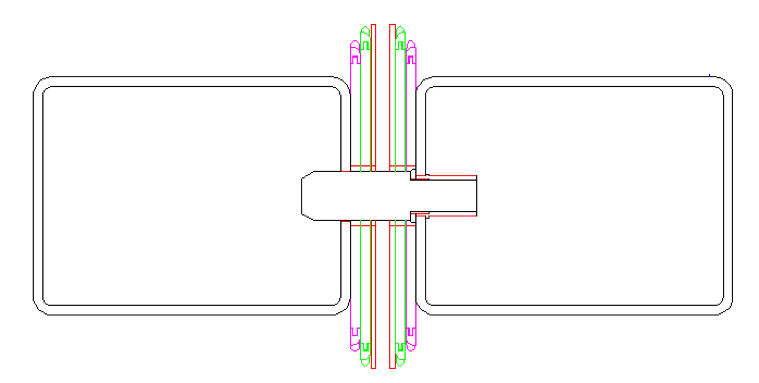
\includegraphics[width=0.9\textwidth]{figures/tpc_apa_pinslotdrawing.png} 
\end{cdrfigure}

Electronics noise concerns have made it desirable to isolate APAs from each other.  Therefore, the alignment pins have G10 sleeves covering their steel cores at places where they come into contact with the frame of the adjacent APA.



%\chapter{det-comp}


%%%%%%%%%%%%%%%%%%%%%%%%%%%%%%%%%%%%%%%%%%%%%%
%\section{Anode Plane Assemblies}

%%%%%%%%%%%%%%%%%%%%%%%%%%%%%%%%%%%%%%%%%%%%%%
\section{Cathode Plane Assemblies}


\subsection{Scope, Requirements and Design Parameters}

The cathode plane is constructed from 6$\times$3 cathode plane assemblies (CPAs) to form the 16m $\times$ 6m area.  It has a HV cup at the beam downstream side to interface with the HV feedthrough. The top and bottom field cage modules are mechanically and electrically connected to the top and bottom edges of the cathode plane.  The cathode plane is suspended through insulating bars to the CPA installation rail.

\subsubsection{Requirements}

\begin{itemize}
\item Provide equipotential surfaces at -180kV nominal bias voltage
\item Maintain a flatness better than 1cm when submerged in the liquid argon
\item Use materials with comparable CTEs to that of stainless steel 
\item Limit the electric field exposed to LAr to under 30kV/cm
\item Prevent damage to the TPC including its readout electronics In case of a HV discharge anywhere on the cathode
\item Provide constant bias voltage and current to all attached field cage resistor divider chains
\item Support the full weight of the 4 connected top/bottom field cage modules and a person on the bottom CPA at installation
\item Accommodate cryostat roof movement between warm and LAr filled states
\item Constructed in modular form that can be easily installed in the cryostat
\item Accommodate PD calibration features
\item Has no trapped volume

\end{itemize}

\subsubsection{Design Parameters}

Width, height, sheet thickness, frame thickness, module width...


\subsection{The need for highly resistive cathode planes}
Stored energy, charge injection to FEE, dominant ionization current density

Summarize key points in DUNE docdb 1320.

\subsection{The Design of the Cathode}

\subsection{Overview}

Introduce the design concept: strong frame with thin resistive cathode surface; field shaping strips cover the frame; HV bus hidden behind the field shaping strips; outer edges of the CPA frame surrounded by the metal profiles used by the field cage.

\begin{cdrfigure}[CPA Concept]{cpa-concept}{The resistive CPA concept. 
 {\bf Left:} A 3d model of a corner of the cathode showing major components {\bf Right:} E field simulation of a portion of the cathode.} 
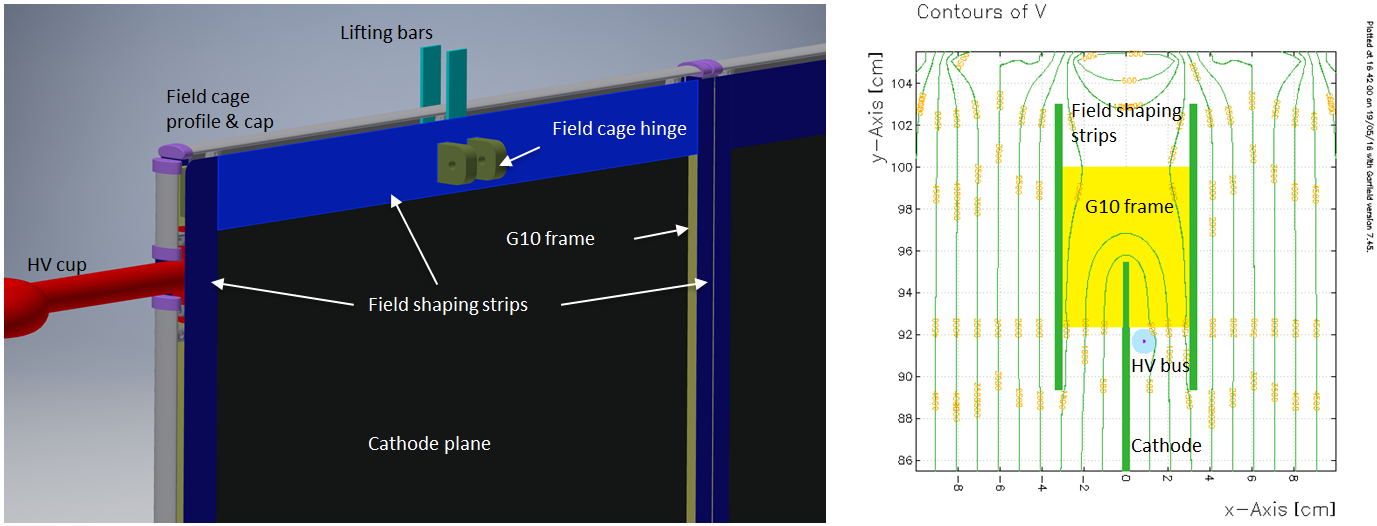
\includegraphics[width=\linewidth]{tpc_cpa_concept.png}
\end{cdrfigure}


\subsubsection{Resistive material}
%% from F. Pietropaolo

The main criteria for the selection of the resistive material to be used for the CPA panels include: 
\begin{itemize}	
\item Surface resistivity range.
\item Compatibility with cryogenic temperatures
\item Robustness to HV discharges, material ageing.
\item Radio-purity.
\item Availability on large area; achievable planarity 
\end{itemize}

Several options have been evaluated.
\begin{itemize}	
\item NORPLEX Micarta NP 315, phenolic laminate loaded with graphite: Intrinsic bulk resistivity in the required range (few M$\Omega$/cm). Density comparable to LAr.
\item Screen printed resistive ink on G10/FR4 substrate (~100 k$\Omega$/square) printed with specific patterns to obtain required average surface resistivity
\item DuPont resistive Kapton film  (25 $\mu$m thickness, graphite loaded, available with resistivity in the 0.5 to 50 M$\Omega$/square range) laminated on G10/FR4 substrate.
\end{itemize}
Also considered at earlier stage:
\begin{itemize}	
\item Zelec ESD powder mixed with polyurethane binder.
\item ESD surface conducting G10 from Current Composite.
\end{itemize}

Radiological tests performed at the LNGS low counting rate facility that G10/FR4 are preferable since MiCarta is more active by orders of magnitude for most relevant radioactive chains.
 
Screen printed ink and Kapton lamination on G10/FR4 are well established fabrication techniques available on panels as large as to 2.1x 1.2 m$^2$ (well matching the CPA panel required size). The screen print technique allows to choose precisely the average surface resistivity value, while Kapton exhibits a more uniform surface and resistivity. 

Tests on large size panels have demonstrated that both options survive without deformation or delamination to repeated immersions in LAr. The resistivity increase at LAr temperature is bounded to less than a factor two for both cases. Electrical contacts are performed with  specific  silver paint paste  highly stable at LAr temperature and resistant to mechanical scratches.

Tests on surface ageing when exposed to HV sparks indicate that Kapton is the preferred solution because:
\begin{itemize}	
\item in the resistive ink case, sparks tend to develop along direction of less resistivity, perpendicular to strip direction inducing a visible degradation of the material surface with some consistent ink evaporation and local measurable change in resistivity (Figure~\ref{fig:cpa-resink}).
\item in the Kapton case instead, sparks are point-like inducing tiny localized carbonization on material surface, at the spark position, but no change in average resistivity is recorded (Figure~\ref{fig:cpa-kapton}). 
\end{itemize}

\begin{cdrfigure}[Resistive ink ageing from sparks]{cpa-resink}{Resistive ink ageing from sparks. 
 {\bf Left:} spark propagation along preferred directions (lower resistivity), {\bf Right:} Status after test: degradation with some material evaporation.} 
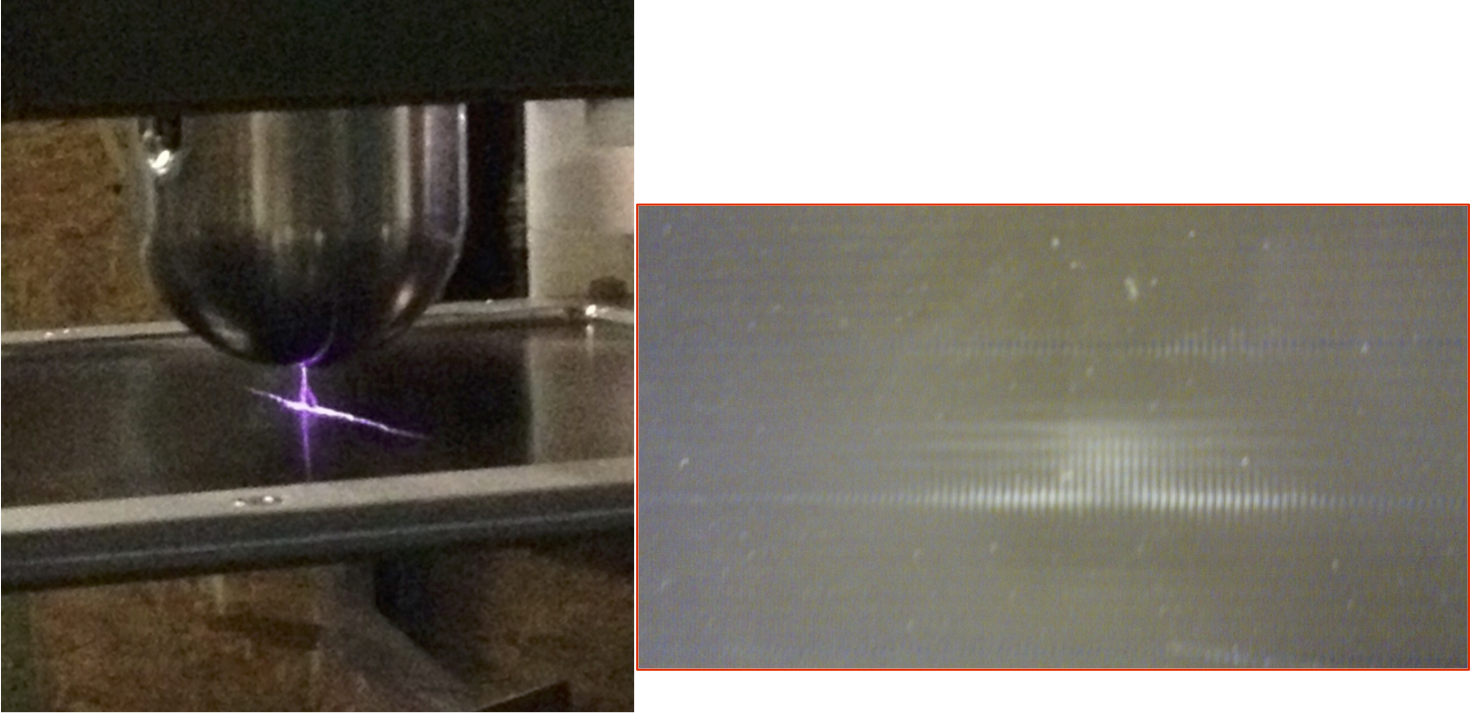
\includegraphics[width=\linewidth]{tpc_cpa-resink.png}
\end{cdrfigure}

\begin{cdrfigure}[The field cage test setup]{cpa-kapton}{Resistive kapton ageing from sparks. 
 {\bf Left:} point-like sparks. {\bf Right:} Localized carbonization on material surface, at the spark position.}
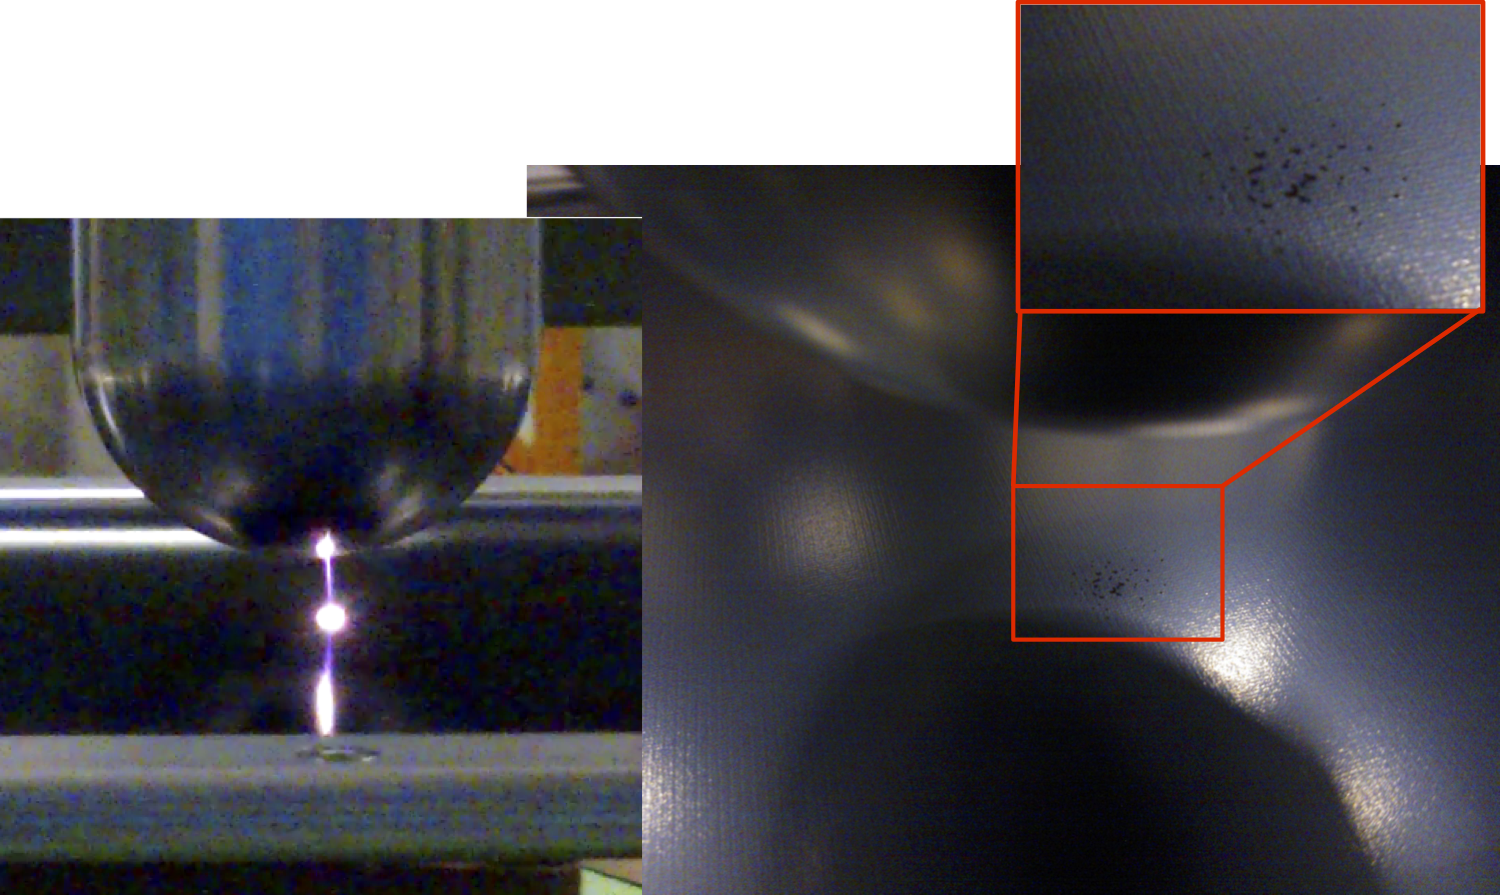
\includegraphics[width=\linewidth]{tpc_cpa-kapton.png}
\end{cdrfigure}

\subsubsection{Support frame material properties}

The main materials for the detector are stainless steel and what is called generically G10 material.  G-10 is a thermosetting industrial fiber glass composite laminate consisting of a continuous filament glass cloth material with an epoxy resin binder. This product, first introduced in the 1950's, has characteristics of high strength, low moisture absorption, excellent electrical properties and chemical resistance. These properties are maintained not only at room temperature but also under humid or moist conditions. NEMA G10 was the designation given to Glass Epoxy sheet composite by the National Electrical Manufacture Association (NEMA) to specify a consistent product between manufactures. 

G10 laminate sheet is made up with difunctional or trifunctional epoxy making up the bulk of heavy sheet and then using finer glass cloth with high temperature resistant tetra-functional epoxy giving a high performance outer finish.

FR4 is the brominated flame retardant version of G 10. The FR 4 material can usually be used where G10 material is specified; however G10 Laminate should not be used where FR-4 is specified.  CERN requires that the material used be flame retardant but halogen free (and therefore bromine free).  FR4 meets the flame retardant requirement but not the halogen free requirement.  Research needs to be conducted into what type of G10/FR4 is available that meets CERN’s requirements.
Another variation of G10 fiberglass sheet is G10 CR laminate used in cryogenic applications. 

Both G-10 and FR-4 are rated at 285 degree F continuous operating temperature. Because they are thermosets, no melting will occur with these grades, however charring will be observed after extended periods above this temperature rating. FR-4 has a UL flammability rating of 94 V-0.

A failure criteria needs to be defined for the G10 material because it is brittle and does not exhibit ductile failure and a defined yield stress like stainless steel.  Brittle materials typically rupture and have a fractional reduction in area due to tensile strain of less than 0.05.  For brittle materials it is recommended that the modified Mohr Theory of Failure be used which states that the principle tensile stresses be less than the ultimate stress of the material.  See Shigley ``Standard Handbook of Machine Design,'' third edition.   Stress concentrations are also a concern for brittle materials and care should be taken to avoid sharp corners and other areas of stress concentrations.  Shigley also defines stress concentration factors which are multipliers for geometric areas where stresses are higher and is a common method for evaluating high stress areas.  

The material properties used for calculations were:

\begin{tabular}{l l}
G10: 	& \\
\hline
Thermal expansion Coefficient	&	$9.6 \times 10^{-6}$ cm/cmK	\\
Modulus of Elasticity			&	2,770ksi				\\
\vspace{0.5em}Ultimate stress				&	32ksi				\\
Stainless Steel: & \\
\hline
Thermal expansion Coefficient	&	$9.6 \times 10^{-6}$ cm/cmK	\\
Modulus of Elasticity			&	30,000ksi				\\
Yield stress					&	36ksi				\\
\end{tabular}


\subsubsection{Mechanical design and stress analysis}

\begin{cdrfigure}[CPA geometry]{cpa-geometry}{Basic geometry of the CPA array, close ups and a CPA column} 
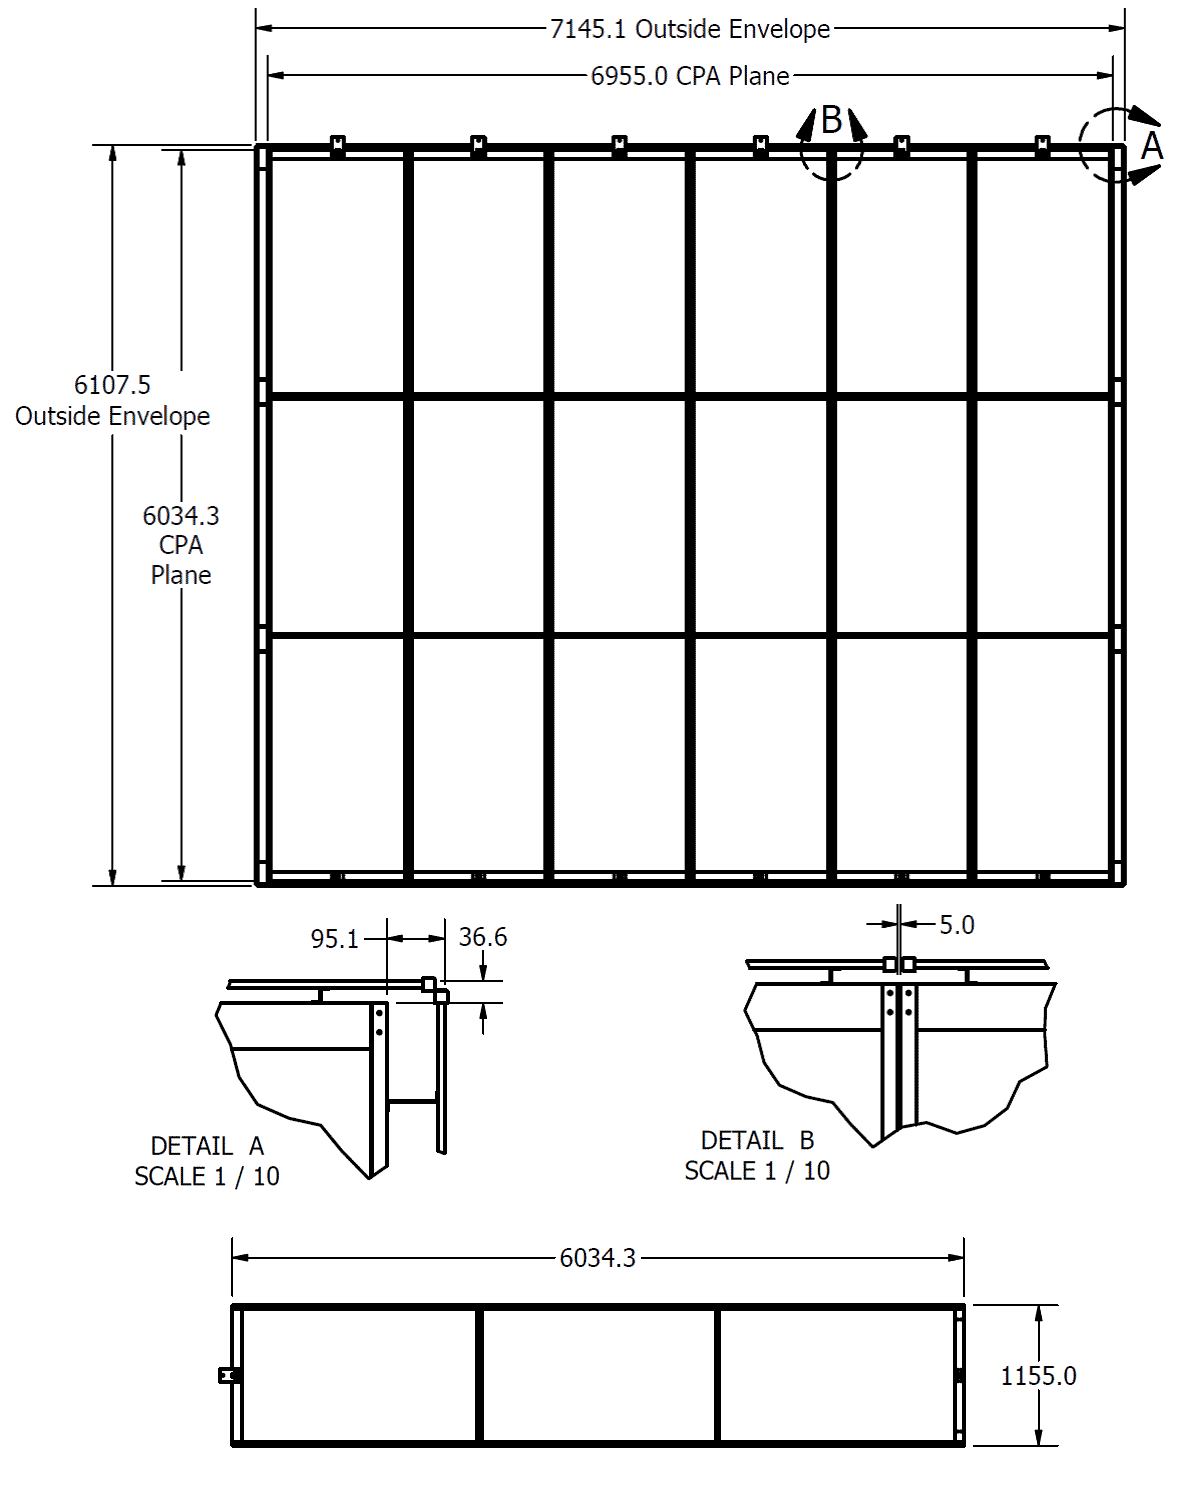
\includegraphics[width=\linewidth]{tpc_cpa_front_views1.png}
\end{cdrfigure}

\begin{cdrfigure}[CPA views2]{cpa-view2}{Views of various part of the CPAs} 
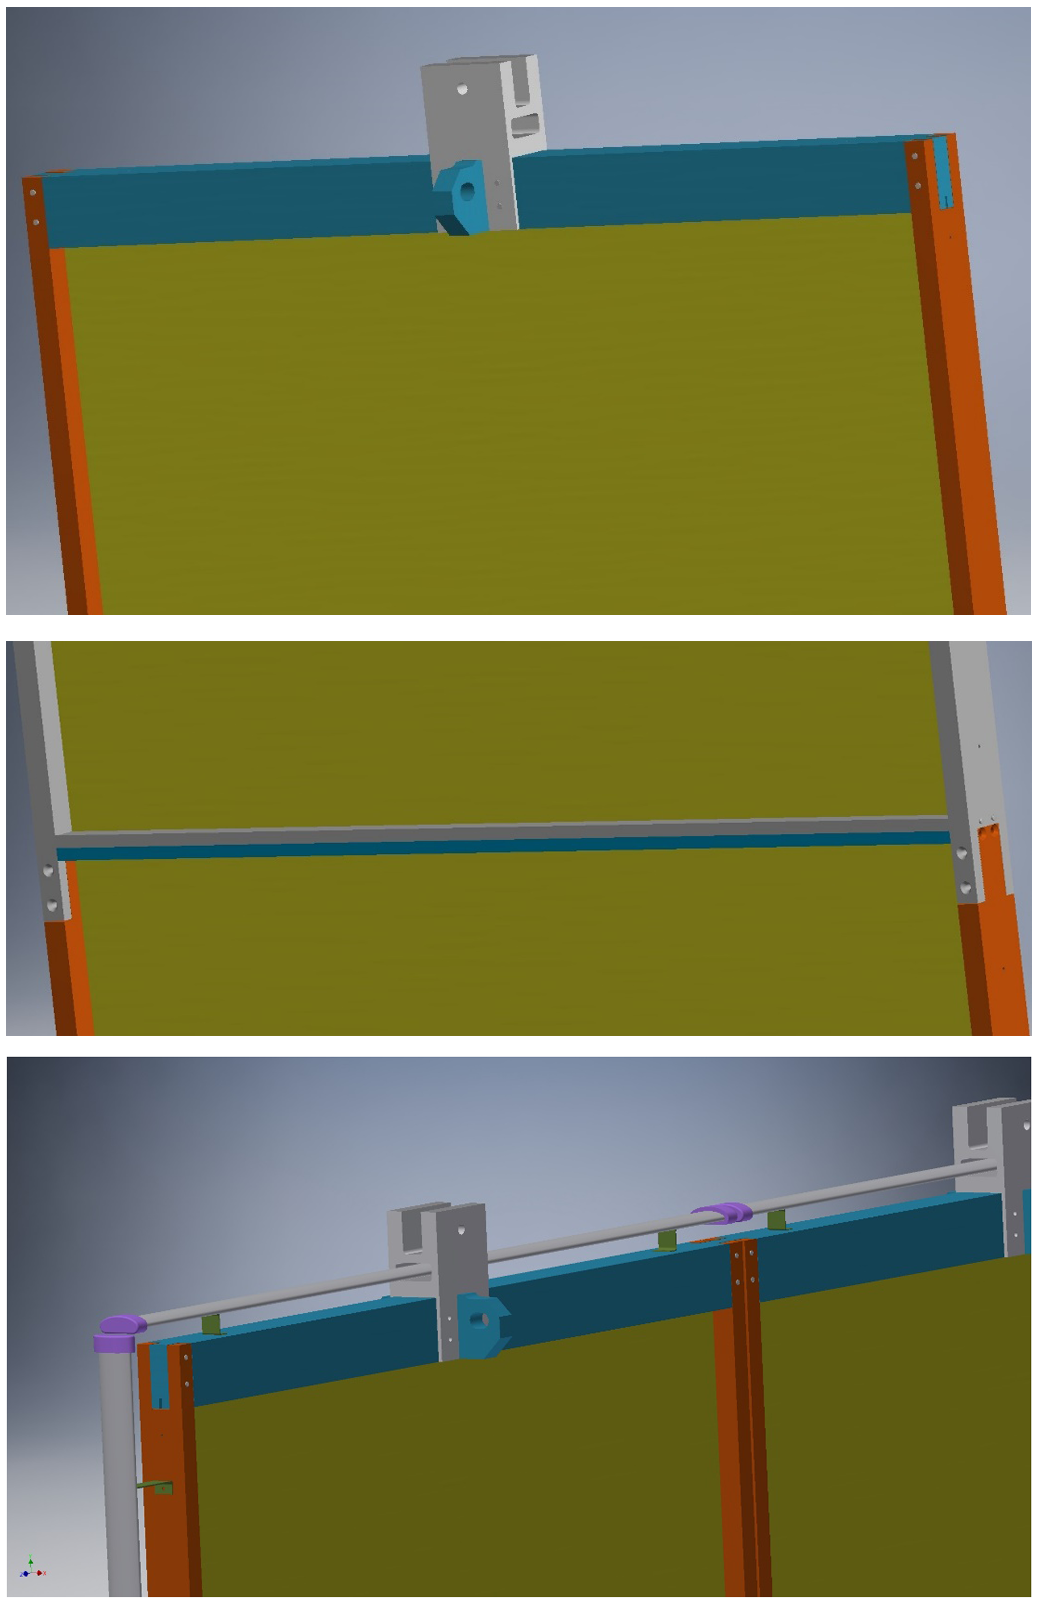
\includegraphics[width=0.8\linewidth]{tpc_cpa_views2.png}
\end{cdrfigure}


Figures~\ref{fig:cpa-geometry} and \ref{fig:cpa-view2} show the basic geometry of the CPA.  The CPA is composed of three modules that are bolted and pinned together with tongue/groove joints to form the full CPA plane.  Each module consists of a framework in which the resistive panel is captured inside a groove.  Each module weights roughly 53 lbs. for a total weight of the CPA plane of 160 lbs.  

The resistive panel is 1/8'' thick G10 and floats within the framework so that no external forces are applied to it.  When hung vertically the weight of the resistive panel (~30lbs per module) rests on the bottom cross bar of the module.  The weight of the modules is transferred through the side bars of the frame and up to the top cross bar, see Figure~\ref{fig:cpa-view2}a.  The very top cross bar of the CPA plane has a block attached to it through which all of the load is transferred to the strap which attaches to the supporting stainless steel I-beam.  

Figure~\ref{fig:cpa-hinge1} shows how the FC will be attached to the assembled CPA plane.  The top and bottom cross bars will have elongated slots through which pins will be inserted to attach the hinged connection.  The weight of the FC is applied to the center of each top and bottom bar.  

\begin{cdrfigure}[CPA and FCA hinged connection]{cpa-hinge1}{The top field cage modules are hung vertically with the CPAs when moved into the cryostat, then rotated to horizontal to attach to the APA} 
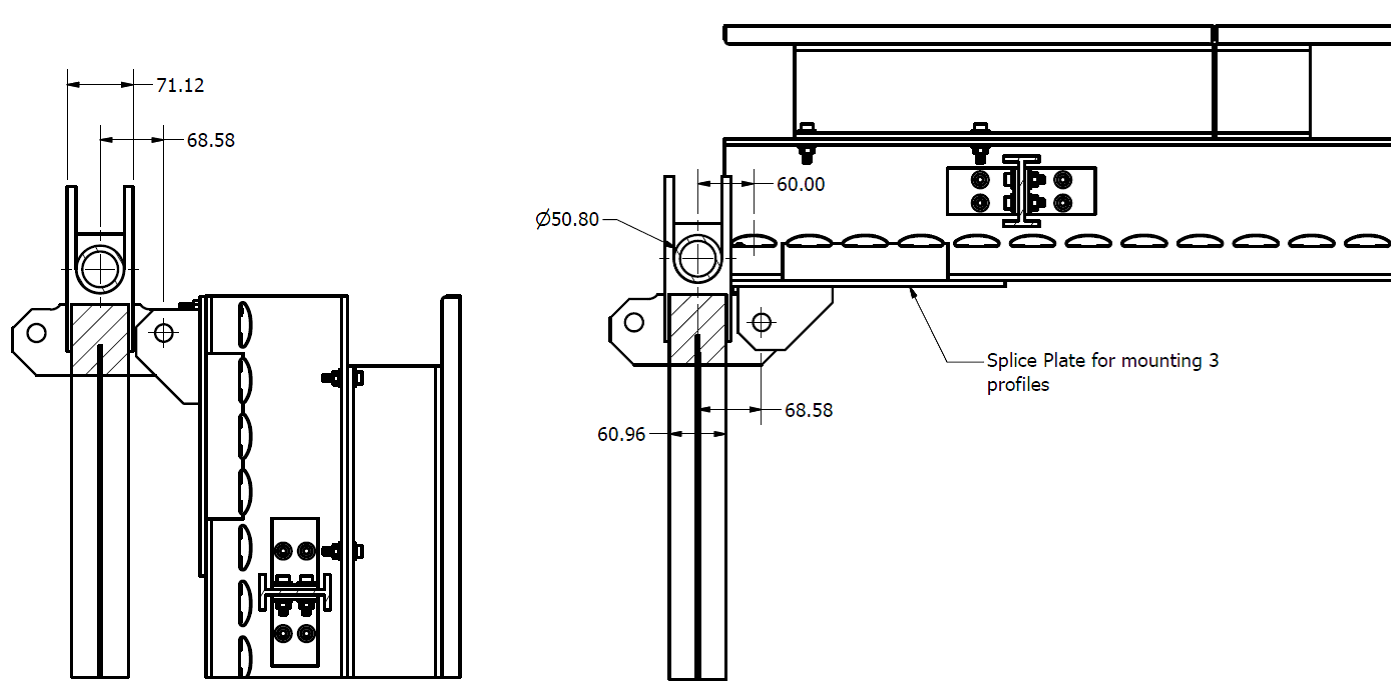
\includegraphics[width=\linewidth]{tpc_cpa_fc_hinge.png}
\end{cdrfigure}


Figure~\ref{fig:cpa-view2}a shows the block at the top of the CPA that is secured to the top cross bar and extends to the top supporting I-beam.  This strap must support the weight of four half FCs (4$\times$220 lbs) and the weight of the CPA itself (160 lbs) for a total weight of 1041 lbs. The section of G10 that connects to the CPA requires and area of only .33 in$^2$ to achieve a safety factor of 10 to the ultimate strength of the G10.  

The strap must have the ability to allow the CPA to pivot and rotate in three directions.  


The CPA frame has been evaluated using empirical and FEA calculations.  The following is a summary of 6 key aspects of the analysis. Detailed calculations are shown in 
\fixme{reference to Vic's writeup}.  

The highest stresses and deflections occur during assembly before the cryostat is filled with liquid.  During installation the CPA must carry the full weight of the FC rather than sharing it with the APA and the buoyancy force which reduces the load from gravity is not present.

In all of the analysis the resistive panels were not included.  In the design of the CPA it is planned that the resistive panel will float within a frame and no load will be applied to it and therefore it does not contribute to the stiffness of the modules.  

{\it A. Lifting the CPA During Installation}

During installation the three frames that make up a CPA module will be placed horizontally on the floor and connected together.  The top of the module will then be secured to the crane and lifted; the bottom of the module will be pivoted on the floor.  By lifting and transversing the hook attached to the top of the module the CPA will be lifted into the vertical position.  The worst case loading occurs immediately after the crane begins to lift the top of the module when it is simply supported at the bottom and top.  The stresses and deflections are small as see in Figure~\ref{fig:cpa-h_load}.   The plane will sag a maximum of roughly 2'' and the stresses are below 2,000psi which is far below the ultimate stress.  

\begin{cdrfigure}[CPA stress in horizontal position]{cpa-h_load}{Stress and deflection of a connected 3 CPA stack in horizontal position supported at both ends} 
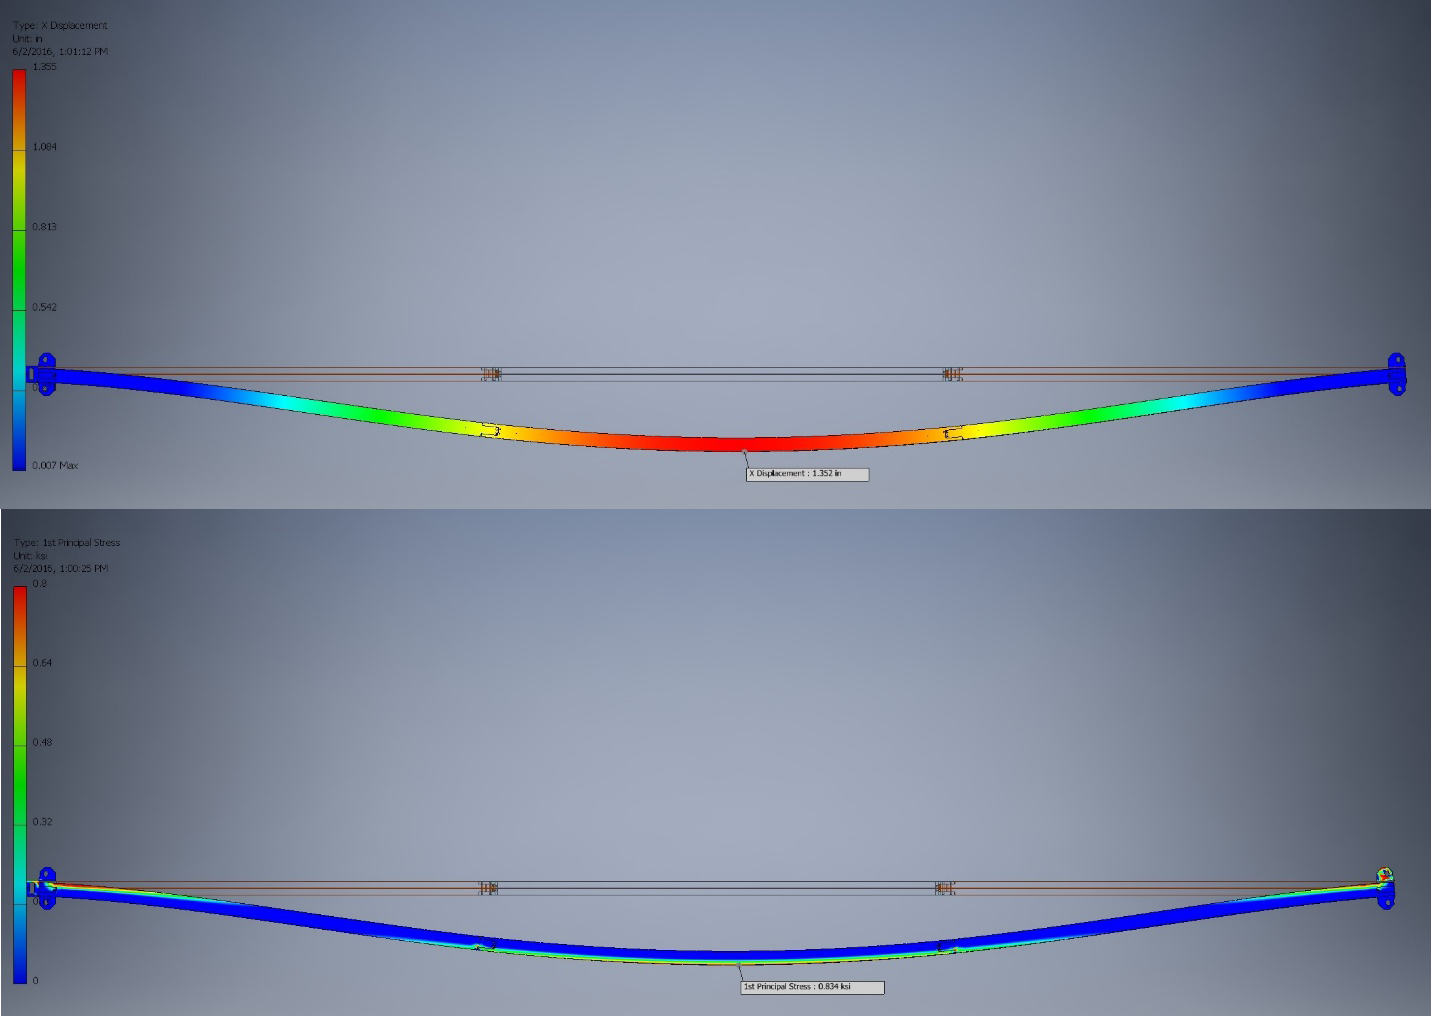
\includegraphics[width=\linewidth]{tpc_cpa_h_load.png}
\end{cdrfigure}


{\it  B. CPA Hanging with all FC Attached in Installation Position}

The current estimate for the FC weight is 440 lbs.  This load is carried by 2 CPAs so each hinge on the CPA will supposed 220 lbs in the installation position.  Figure~\ref{fig:cpa-load1} below shows the deflections and maximum stresses.  The larges deflections are at the bottom cross bar of 0.07'' and the stresses are less than 2,000psi which is far below the ultimate stress of G10.

\begin{cdrfigure}[CPA and 4 FCA load]{cpa-load1}{Stress and deflection of a connected 3 CPA stack suspended on the rail with 4 FC modules} 
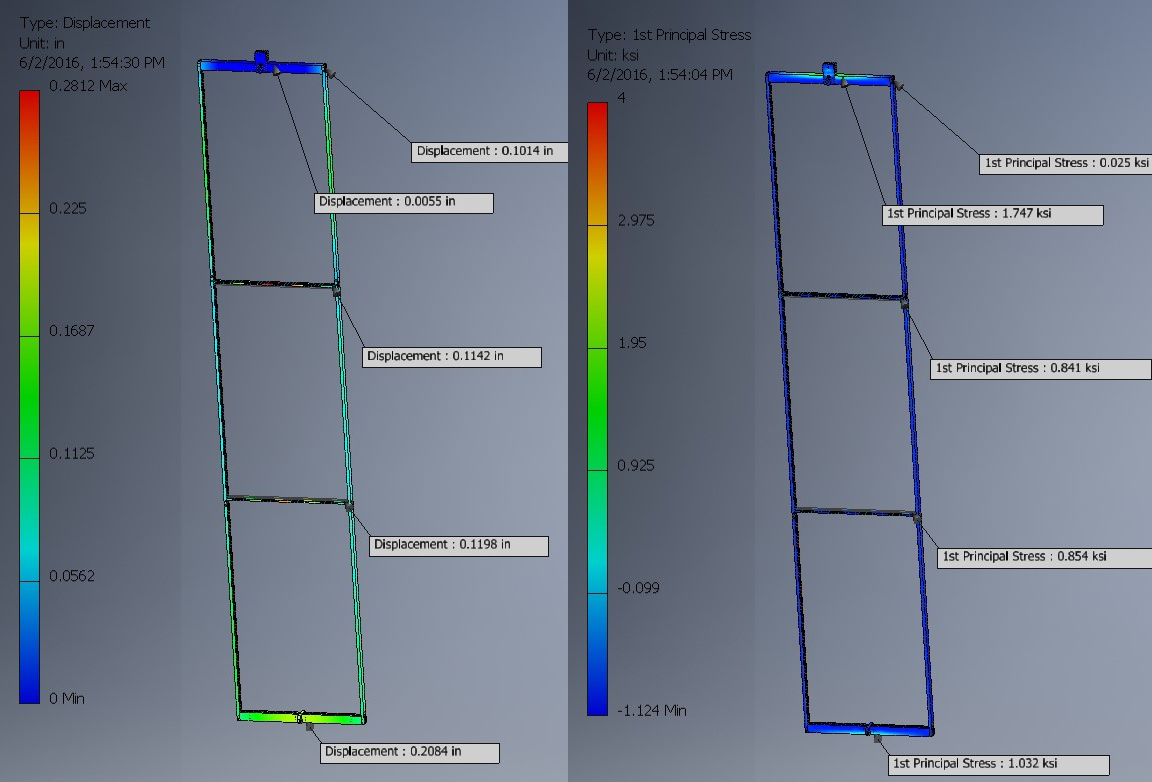
\includegraphics[width=\linewidth]{tpc_cpa_fc_load1.png}
\end{cdrfigure}


{\it  C. CPA Hanging with all FC Attached in Deployed Position With Weight of Workers on FC}

The current estimate for the FC weight is 440 lbs.  This load is carried by 2 CPAs and by the APAs so each hinge on the CPA will supposed 110 lbs in the installation position.  In addition, in the worst case a 200 lbs worker could be standing directly over an I-beam on the FC directly next to a CPA.  The top two hinges on the CPA will have 110 lbs applied.  One of the bottom hinges will have a 110 lbs load also and the second bottom hinge will have 110 lbs of the FC plus the 200 lbs of the worker applied.  The largest deflection is 0.1'' at the bottom cross bar and the stresses are less than 2200psi which is far below the ultimate stress of G10.

\begin{cdrfigure}[CPA load plus 200lb]{cpa-load2}{Stresses and Deflections of CPA with FC Deployed and 200 lb Worker Load} 
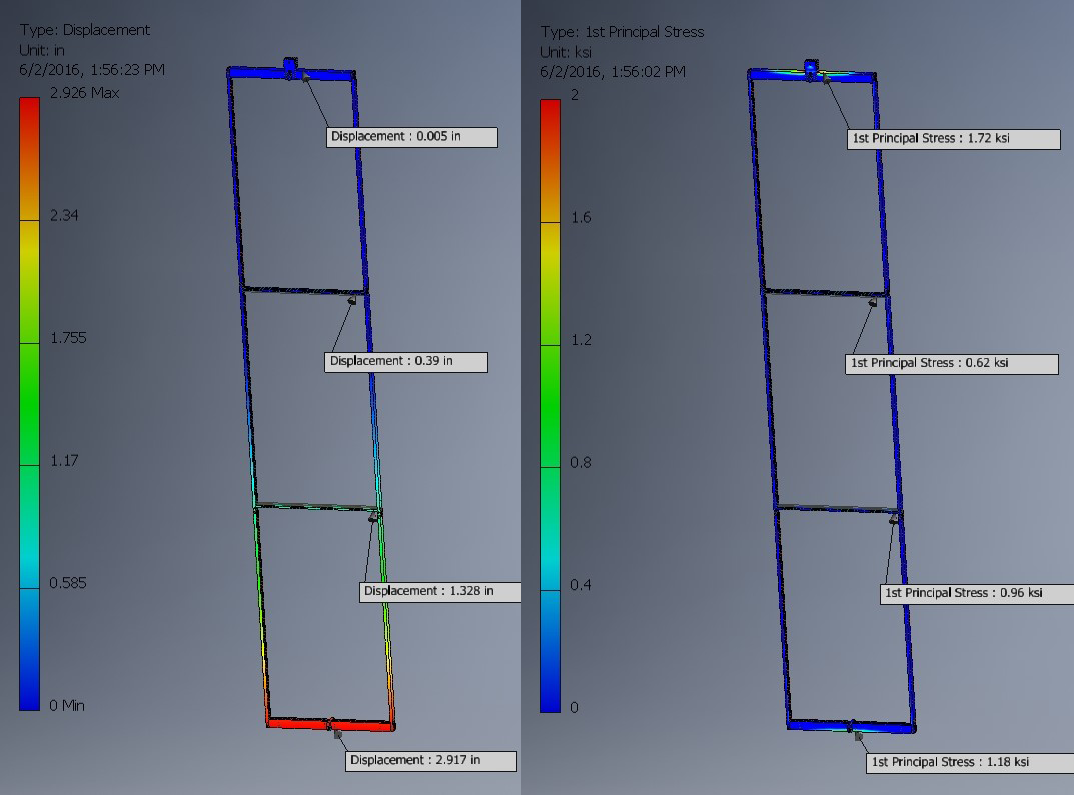
\includegraphics[width=\linewidth]{tpc_cpa_fc_load2.png}
\end{cdrfigure}

{\it D. Connection Stresses}

The weight of the CPA and the bottom FC is transferred through the side bars of the CPA frame.  The connection between the side bars and the top cross bar therefore will experience the highest loads.  A single 1/4'' diameter G10 pin at the connection would have a shear stress of 7740psi which provides a safety factor of greater than 4.  A second pin at each connection would increase the safety factor to 8.  

{\it E. Deformation and Stress Due to Pressure from Circulating Liquid Argon}

Calculations done at FermiLab indicate that a uniform 2Pa pressure during cool down will be applied to the resistive panels.  Calculations show that this will result in 0.090'' deflections of the panel at its center.  The CPA/FC/APA assembly will displace 8.8mm laterally as a result of the next force from this pressure.  

{\it F. Thermal Considerations}

When the CPA modules are cooled their width will shrink by 0.9mm.  The supporting stainless steel beam will shrink by 1.6mm over the width of the CPA.  If the CPA supports are rigidly attached to the supporting stainless steel beam then an interference of 1.6m-.9mm = .7mm will occur.  In order to prevent this interference an initial gap of 0.7mm between CPA’s is required which will insure that the CPAs are in contact after cool down.  

The steel beam between the CPA and APA will cool and shrink by 5.2mm.  The joint between the FC and the CPA must be able to accommodate this shrinkage.


\subsubsection{The HV distribution bus and HV feedthrough receptacle }

Should this be moved to the HV section?

\subsubsection{The mechanical and electrical interconnect features between modules}

There are a stack of 3 modules interconnected vertically to form the 6m height of the SP ProtoDUNE cathode.  The frames of these modules are bolted together using tongue and groove connections at the ends, and the resistive cathode sheets, and the field shaping strips are connected  using a few metallic buttons to ensure redundant electrical contact between vertical modules.

There are 6 columns of the 6m tall CPA modules in SP ProtoDUNE.  Each column is suspended to the CPA rail using a central lifting bar.  Due to the  roof movement between the warm and cold phases of the cryostat, each column is expected to move ~ 2mm relative to its neighbors.  Several pin and slot connections are implemented at the long edges of the CPA columns to ensure the co-planarity of the modules and yet allow small vertical displacement.  The HV bus interconnect the resistive cathode surfaces across the columns to maintain a uniform voltage across the cathode surface.

\subsection{QC Procedures}


%\chapter{det-comp}


%%%%%%%%%%%%%%%%%%%%%%%%%%%%%%%%%%%%%%%%%%%%%%
%\section{Anode Plane Assemblies}

%%%%%%%%%%%%%%%%%%%%%%%%%%%%%%%%%%%%%%%%%%%%%%
%\section{Cathode Plane Assemblies}

%%%%%%%%%%%%%%%%%%%%%%%%%%%%%%%%%%%%%%%%%%%%%%
\section{Field Cage}
\label{detcompsec-fc}
%%%%%%%%%%%%%%%%%%%%%%%%%
%\subsection{Scope, Requirements and Design Parameters}
\subsection{Overview and Requirements} 

In the TPC, each pair of facing cathode and anode planes forms an electron-drift region. A field
cage (FC) must completely surround the four open sides of this region to provide the necessary boundary
conditions to ensure a uniform electric field within, unaffected by the presence of the cryostat walls.

The FCs are constructed using multiple copper-clad FR-4 sheets reinforced with fiber
glass I-beams to form modules of 2.3 m $\times$ 3.6 m in size. Parallel copper strips are etched on
the FR-4 sheets using standard printed circuit board fabrication techniques. Strips are biased at
appropriate voltages provided by a resistive-divider network. These strips create a linear electric potential
gradient in the LAr, ensuring a uniform drift field in the TPC active volume. Simulations
have shown that the non-uniformity of the drift field quickly drops to about 1\%, roughly a strip
pitch away from the field-cage surface.
\fixme{The above taken from sec 4.3.4 of the detector volume of the CDR as an intro. May need update for protodune-sp?? Anne}

The FC is required to:
\begin{itemize}
\item provide the nominal drift field of 500V/cm;
\item withstand $-$180kV near the cathode;
\item define the drift distance between the APAs and CPAs to <1~cm;
\item limit the electric field in the LAr volume to under 30~kV/cm;
\item miminize the peak energy transfer in case of a HV discharge anywhere on the field cage or cathode;
\item provide redundancy in the resistor divider; \fixme{this feels incomplete... ``in the resistor-divider chain?}
\item maintain the divider current much greater than the ionization current in the TPC drift cell, yet less than the power supply current limit when all dividers are connected in parallel;
\item be modular in form such that they can be easily installed in the cryostat;
\item provide support for the beam plug;
\item allow calibration laser beams to enter into the active volume; 
\item support a 200-lb. person standing on the support beam of the bottom field cage module;
\item be configurable to either 3.6~m or 2.5~m drift length inside the cryostat; and
\item prevent any trapped volume.
\end{itemize}

%%%%%%%%%%%%%%%%%%%%%%%%%
\subsection{Mechanical design}

The ProtoDUNE-SP TPC will have six top and six bottom FC assemblies, arranged three across each horizontal edge of the two drift regions. It will have 
four end-wall panels, one at each vertical edge of the two drift regions, see Figure~\ref{fig:fc-overview} and~\ref{fig:fc-endwall_module}.
Each endwall panel consists of four assemblies in ``landscape'' orientation, stacked vertically.
FC assemblies are constructed from pultruded G10 I-beams and box beams that support extruded field-shaping aluminum profiles. The support structure for each of the top and bottom FC assemblies consists of two main I-beams that are 3.6~m long, and three cross I-beams that brace the main I-beams for structural stability.
\fixme{One field cage with many assemblies or modules? Clarify assembly vs module} 


\begin{cdrfigure}[An end wall field cage module]{fc-endwall_module}{A view of an end wall field cage module}
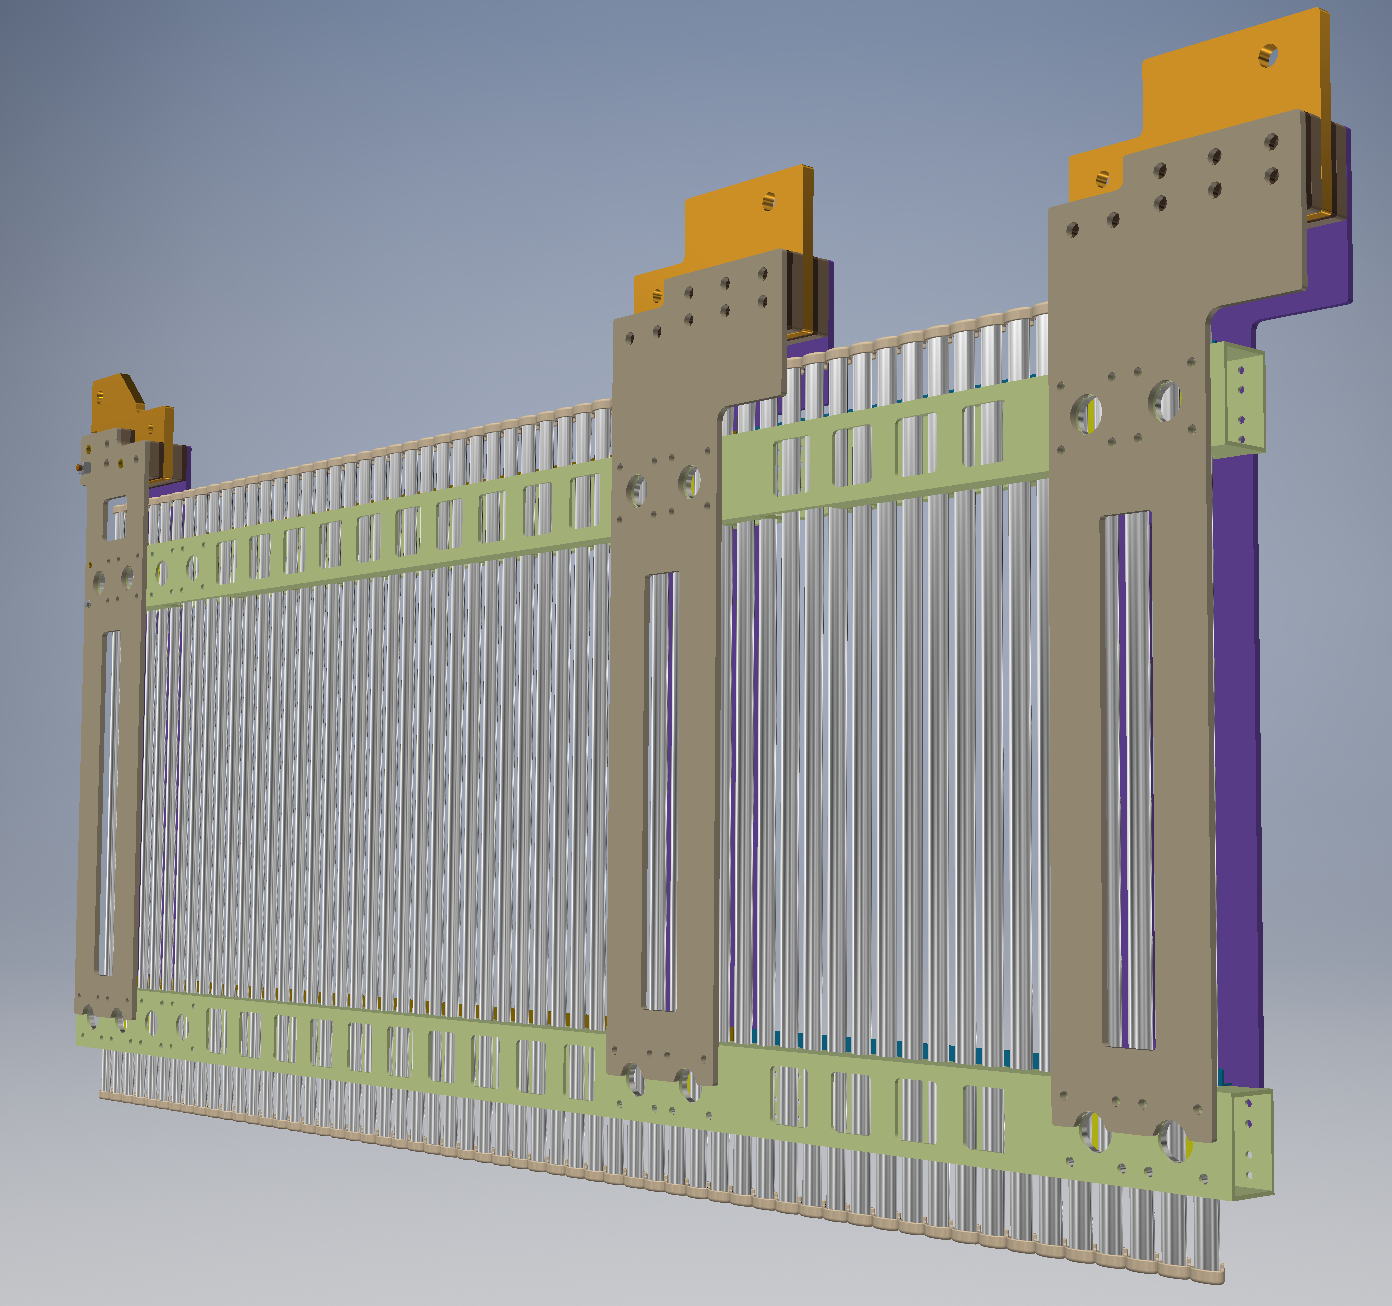
\includegraphics[width=0.8\linewidth]{tpc_fc_endwall_module.png}
\end{cdrfigure}

The main I-beams have cutouts to hold the field-shaping profiles. Main I-beams are spliced at 2.5~m to facilitate drift distance  
of 2.5~m. Splice joints and cross I-beam joints are held together using an arrangement of shear pins and plates. 

Aside from the profiles themselves, the nuts and bolts holding them, and the ground planes, all FC components are made of insulating material. The material selected for these structural components is fiberglass-reinforced plastic (FRP), which will prevent binding when the structure is at cryogenic temperatures. The ground planes are made of stainless steel. 

\fixme{from docdb 1504 sec 6.3 I can't tell if there's ONE ground plane at the TOP, ONE at the BOTTOM or two. In this section it appears plural. 1504 needs clarification. }

The inward-facing face of the ground planes will be approximately 20~cm away from the top of the field-shaping profiles. The ground planes are mounted at a fixed distance from the field shaping profiles by standoffs, as shown in Figure~\ref{fig:fc-with-ground-planes}, which shows ground planes over I-beams and cross beams.

\begin{cdrfigure}[The field cage with ground planes]{fc-with-ground-planes}{The field cage with ground planes}
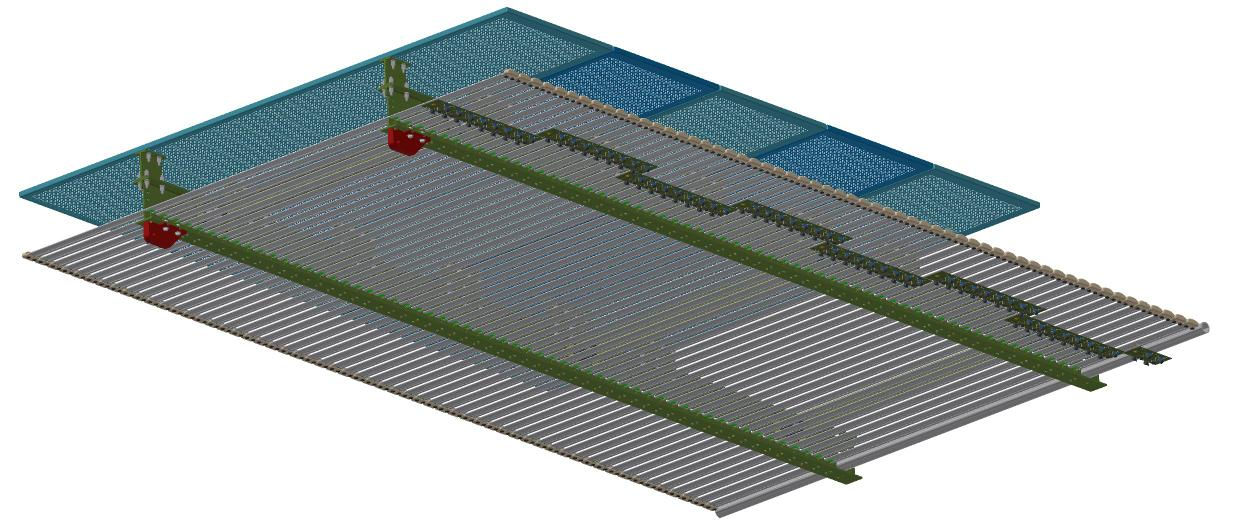
\includegraphics[width=0.8\linewidth]{fc-with-ground-planes}
\end{cdrfigure}

The parallel metal profiles in each FC assembly 
 are interconnected by a resistive divider chain, and supported by the FRP beams that span the drift distance.  Between adjacent field cage assemblies, however,  
the metal profiles are neither mechanically nor electrically connected. Gaps between assemblies range from a few millimeters to a few centimeters are designed into the TPC assembly to ensure sufficient clearance for the installation.  The electrical isolation between the field cage modules minimizes the peak energy dump in case of a HV discharge.


%%%%%%%%%%%%%%%%%%%%%%%%%
\subsection{Electrical design}

Given a large standoff distance between the FC and the grounded cryostat wall, it is relatively easy to design a FC that meets the 30-kV/cm E field limit with 180-kV bias.  However, It becomes challenging to reduce the clearance between the FC and ground in order to make more efficient use of liquid argon.  This requires an electrode with a low profile, rounded edges, no trapped volume, and low cost.  Several commercially available roll-formed metal profiles were studied and appear to meet these requirements. \fixme{what's challenging about it then?}

Figure~\ref{fig:fc-schematic} is a schematic of the electrical design of  the CPA and a top/bottom field cage module pair.

\begin{cdrfigure}[Field cage schematic diagram]{fc-schematic}{A schematic diagram of the CPA and a top/bottom field cage module pair}
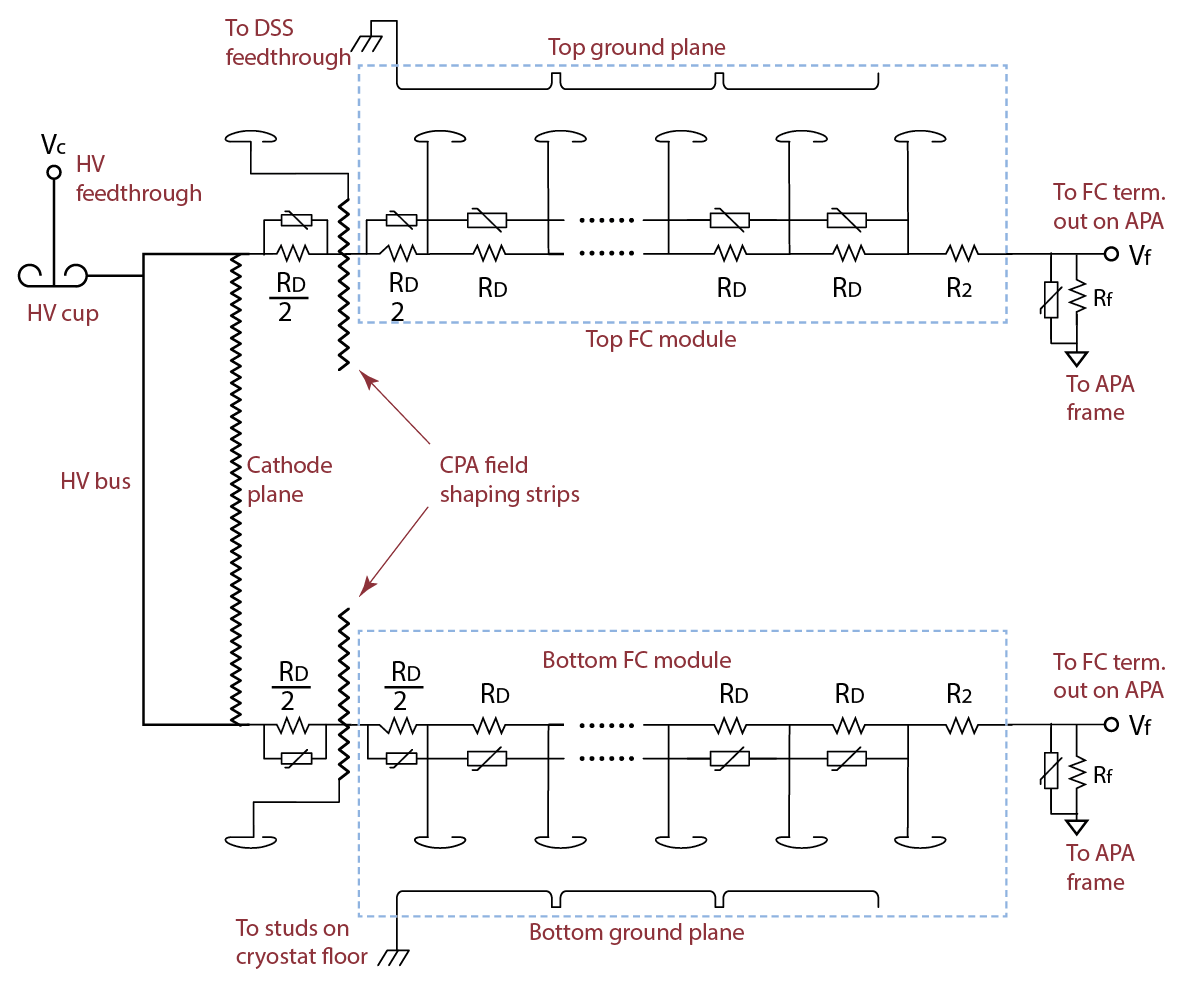
\includegraphics[width=0.8\linewidth]{tpc_fc_schematic.png}
\end{cdrfigure}

%%%%%%%%%%%%
\subsubsection{Electrostatic analysis}

The Dahlstrom Roll Form \#1071 was found to have the lowest surface E field, which was about 12~kV/cm when biased at 180~kV with only a 20-cm ground clearance (see Figure~\ref{fig:fc-profile1071}).

\begin{cdrfigure}[2D FEA of roll formed profiles]{fc-profile1071}{A 2D FEA of a configuration using profile 1071, and a conceptual design of the field cage module}
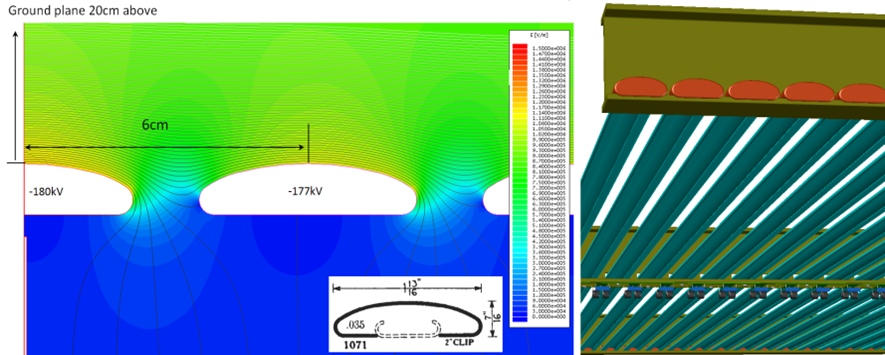
\includegraphics[width=0.8\linewidth]{tpc_fc_profile1071.png}
\end{cdrfigure}
  
In order to maintain a modular design of the field cage while minimizing peak energy transfer in a discharge, the field cage will be constructed with electrical isolation between neighboring modules. If a discharge occurs on one field cage, the electrodes from the neighboring modules will not arc over and cause a domino effect.  This requires a 
electrical insulation between profile ends of the order of 180~kV.  UHMW PE caps of 5-mm thickness are placed over both ends of each profile to serve this purpose. This technique also limits the exposed electric field in LAr at the corner of the field cage, see Figure~\ref{fig:fc_corner}. 

\begin{cdrfigure}[3D FEA of field cage corner]{fc_profile_corner}{A 3D FEA of a field cage corner.  The PE caps (in outline form) limit the exposed E field below the 30kV/cm threshold.}
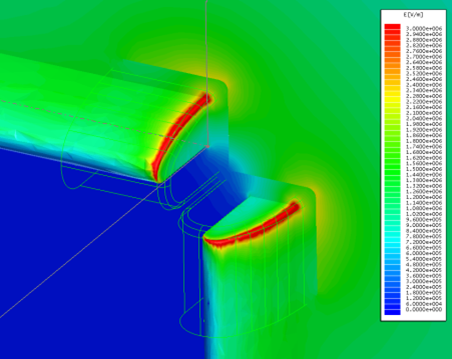
\includegraphics[width=0.6\linewidth]{tpc_fc_profile_corner.png}
\end{cdrfigure}

The center-to-center distance between the profiles is set to 6~cm, and the inner surface of all profiles on a field cage module is placed 5~cm beyond the nearest surface of the TPC active volume (defined by the APA active aperture over the drift distance). The E field uniformity at the edge of the active volume is expected to be within $\pm$2\% of the nominal value.


%%%%%%%%%%%%  
\subsubsection{Surge suppressor on FC}

\fixme{Not clear what design will be used; discusses alternatives}

The resistors along the divider, Figure~\ref{fig:fc-divider-view}, provide a linear DC voltage gradient. However, at shorter time scales ($\ll$1~s), the electrical behavior of the divider is determined by the various capacitances on and between each electrode, and  is no longer linear at this time scale. 

\begin{cdrfigure}[The resistive divider]{fc-divider-view}{A view of a resistive divider}
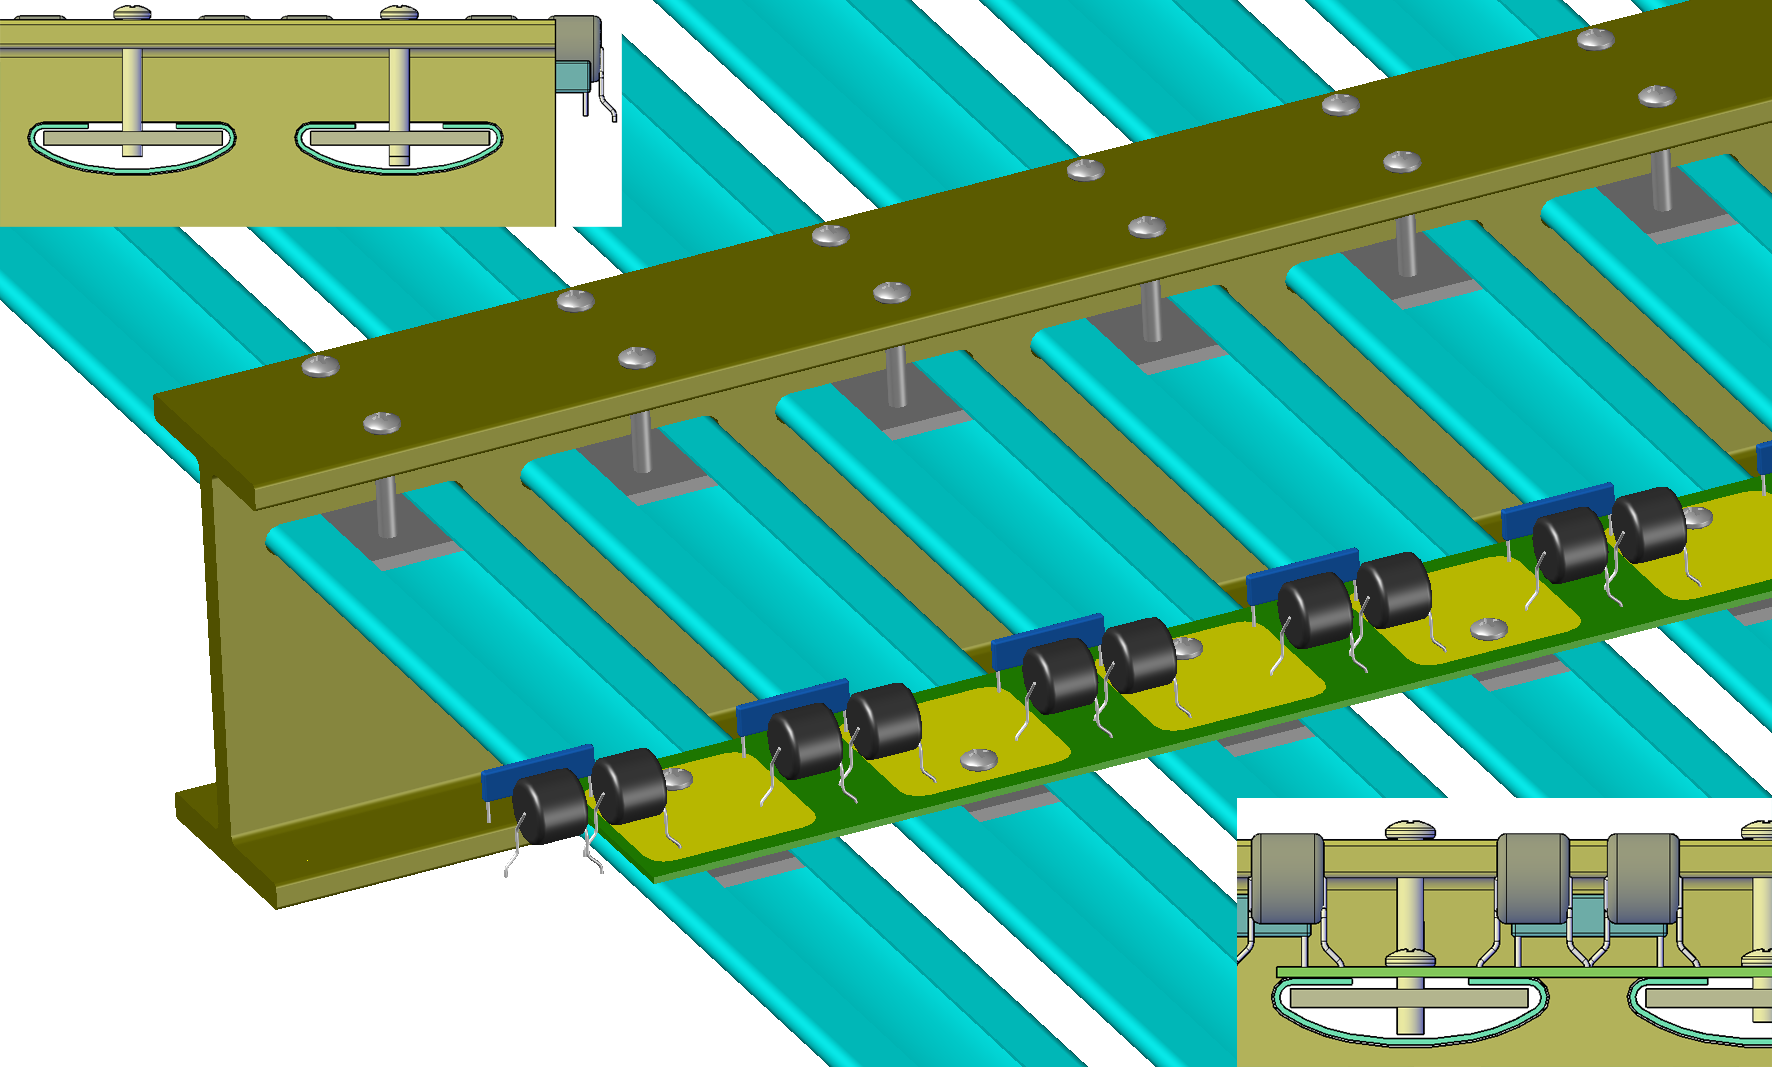
\includegraphics[width=0.8\linewidth]{tpc_fc_r_divider.png}
\end{cdrfigure}

A perfect capacitive divider requires the capacitance of each node to ground to be zero.  In reality, there is always a finite capacitance from each node to ground, and these capacitances resist change in the voltages on the nodes. In the event of a HV breakdown between the cathode and ground (cryostat), the cathode voltage quickly collapses to ground, but the first FC electrode-to-ground capacitance keeps its voltage from changing instantaneously to follow the cathode voltage, resulting in a momentarily larger voltage differential between the cathode and the first FC electrode. This voltage differential can be a significant fraction of the cathode operating voltage, large enough to cause HV breakdown between the two electrodes, or worse yet, to destroy the divider resistors between the two electrodes.

A natural solution to this problem is to significantly increase the capacitance between the nodes of this divider. This was the approach adopted in the 35-ton prototype's field cage through the use of double-sided printed circuit boards (PCB).  However, the cost of the PCB version of the field cage at DUNE scale is very high, and adding discrete HV capactitors between divider taps is also expensitive.

An alternative is to use surge surpressors in parallel with the divider resistors to divert the transient current from the resistors. Extensive tests have been done by MicroBooNE (docdb 3242, arXiv:1406.5216v2) \fixme{add in bib and cite here} on the use of metal oxide varistors (MOVs) and gas discharge tubes (GDTs) as a means of limiting the over-voltage condition in the event of a HV discharge in the TPC. 

Both types will work for the purpose of restricting the voltage differential between field cage rings in LAr temperature. 
A GDT quickly shorts the terminals when the voltage differential exceeds a threshold, while
a varistor changes its resistance to keep the voltage differential near the threshold voltage.
The smooth transition and well defined clamping voltage of the varistors are preferred to the abrupt switching of the GDTs.
The varistors could also function as redundant ``resistors'' in a divider chain in case a resistor is open circuit. \fixme{open circuited?}

One readily available MOV famility \fixme{family?} with high threshold voltage is the Panasonic ERZ-VXXD182.  These have a threshold voltage around 1600~V.  Two of these in series could work with the current 3-kV differential between divider taps.  However, this configuration would not allow raising the E field much above the nominal 500~V/cm.  To allow some headroom in operating field, three such MOVs in series would be needed.

%%%%%%%%%%%%%%%%%%%%%%%%%
%\subsection{Validation tests of roll-formed FC design}


\begin{cdrfigure}[The field cage test setup]{fc-test}{The field cage test setup. 
 {\bf Left:} schematic drawings of the cage showing the main elements: metal profiles, I-beams, ground planes.
  {\bf Right:} Picture of the realized setup.}
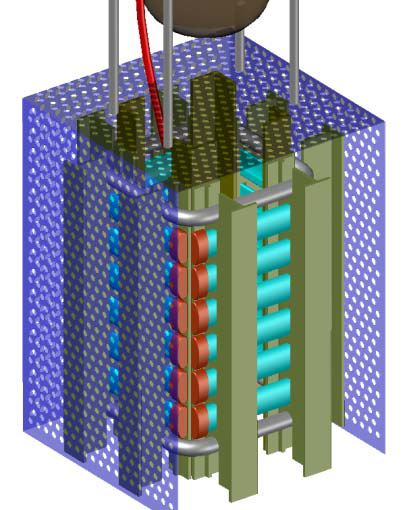
\includegraphics[width=0.45\linewidth]{tpc_fc-test-1.png}
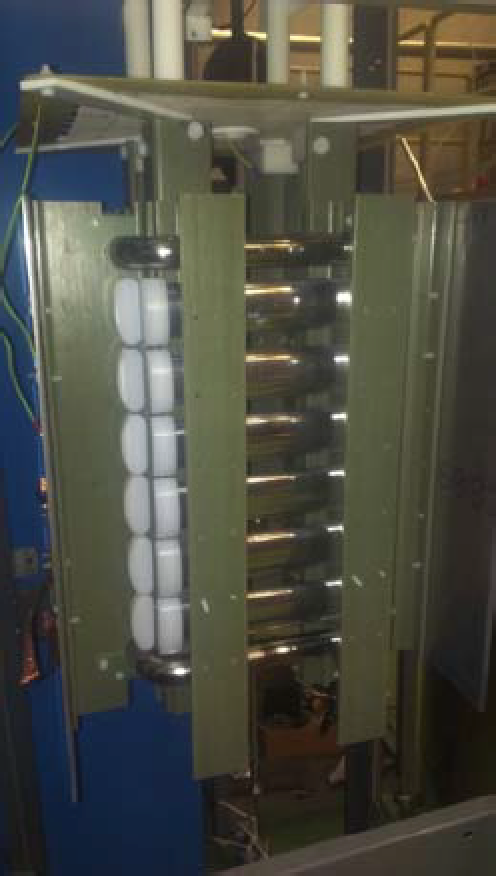
\includegraphics[width=0.45\linewidth]{tpc_fc-test-2.png}
\end{cdrfigure}
\fixme{Remove Figure~\ref{fig:fc-test}? Not shown as ``remove it'' in Gina's printout}


%%%%%%%%%%%%%%%%%%%%%%%%%
\subsection{Ground plane design}
%% by A. Zani

In order to confine the electric field in the liquid argon region, it is foreseen to install a grounded metallic plane,  between the upper field cage module and the liquid-gas interface. The design of such a Ground Plane (GP) \fixme{need to define acronym above and just use it} is inspired by the one from the ICARUS T600 detector, and it is meant to limit the residual electric field in the liquid below the usual 30~kV/cm value. 
\fixme{Is it to keep the E field from going outside the LAr volume or is it to keep the residual field that's already in the LAr volume very small?}
%The design details of the planes were verified to comply with the requests on residual electric field with FEA.  It is noted that a similar GP could be added in front of all the other Field Cage (FC) modules, in order to smooth the field in the LAr dead volume. However, so far it is foreseen to add an actual GP only below the bottom FC, to further smooth the field in the region where pipings for the cryostat filling are running. The distance between the cryostat walls and the end-wall field cage does not require to insert a GP, instead.
The design details of the planes were verified for compliance with the requests on residual electric field with FEA. \fixme{I cannot parse prev sentence} 

In the ProtoDUNE-SP configuration, the GP will be put at a distance of 200~mm from the FC profile, with a structure of $6$ mm holes, $10$ mm pitch ($\sim 25\%$ transparency): the lower fraction of pierced surface is verified by simulations to maintain the field within the required values. The edges of the plates, $20$ mm high, are rounded at $5$ mm, while the holes rounding radius, at production is around $0.5$ mm. The liquid level is expected to be at 40 mm above the GP bottom, i.e. 20 mm above the edges. The radius of curvature for the holes is not a strict requirement. It depends on the punching technique, and usually is at around $0.5$ mm. The actual requirement is to have the hole curvature on the inside (of the TPC) looking out.
\fixme{The previous pgraph needs clarification}

Two sets of pieces \fixme{two sets of GPs? Define ``piece''} were initially produced in Europe:
\begin{itemize}
\item 8 pieces of dimension $198 \times 571$ mm (weight $< 1$ kg each) to be installed in the CERN field cage prototype,
\item 6 more pieces of  $525 \times 2318$ mm (weight around $8.5$ kg each), which represent full scale components for ProtoDUNE-SP. %The drawing of this second set of pieces, sent to the U.S. for test assemblies, in shown in Figure~\ref{fig:gp_panels}. -- this figure was removed per Gina
\end{itemize}



%%%%%%%%%%%%%%%%%%%%%%%%%
\subsection{Field cage and ground plane modules}

%The design details of the FC+GP modules for ProtoDUNE is described and shown in the next section. 
One field cage and ground plane (FC+GP) module will be made of six pieces, aligned 
along their long (2318-mm) dimension 
 in order to match the APA and FC module widths. The planes are connected to the FC beam with additional 
G10 pieces that are also used to connect adjoining 
GP panels. \fixme{piece vs panel?}

Figure~\ref{fig:fc_full} shows a 3D model of one fully assembled FC+GP module.

\begin{cdrfigure}[CERN Prototype]{fc_full}{3D model of one fully assembled FC+GP module, for the top of the field cage. }
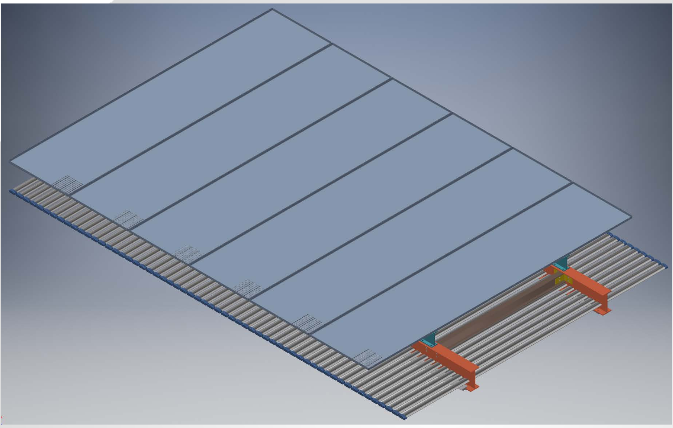
\includegraphics[width=0.8\linewidth]{tpc_topFC.png}
\end{cdrfigure}

The electrical continuity between consecutive panels can be made 
with metallic screws (with holes on the planes edges) or with looser connections, e.g., copper strips, that better adapt to the shrinking of the structure during cooldown. 
As for most detector systems, the GP will %should 
be referenced to the detector ground, located 
at the cryostat top.

The GP modules \fixme{modules or panels?} will be installed on their corresponding FC modules in the clean room outside the cryostat, to facilitate the connections. The description of how the top/bottom FC modules are assembled and connected to the CPA before insertion in the cryostat is provided in Section  \fixme{need to find and add reference}.

Further GP panels need to be attached to the top FC module:
\begin{itemize}
\item Smaller panels will have to be connected on the modules on one side of the CPA so that, once in position, they 
cover the CPA frame. Their dimensions are 
still to be defined, depending on the final design of the CPA hanging scheme. Such \fixme{the same pieces are connected, or similar ones are?} pieces should also be connected to the modules covering the opposite drift region, when in final position.
\item An additional 
set of small panels should be installed on the outer modules of the FC to extend the GP over the vertical FC walls, which will  
further constrain the electric field in these regions. A FEA 
shows that the optimized overhang distance is 20~cm, provided LAr is at 40~mm above the bottom of the GP. The maximal residual field in this configuration is of the order of 13~kV/cm, with less than 1~kV/cm field in the gas phase.
\end{itemize}

%%%%%%%%%%%%%%%%%%%%%%%%%  -- these sections are not needed. I moved the little text there was up, along with the figures. Anne.

%\subsection{Designs of the Field Cage Modules}

%%%%%%%%%%%%
%\subsubsection{Top and bottom modules}

%The main structure of the top/bottom field cage, constructed of two main I-beams that are 3.6-m long, and four cross I-beams that connect main I-beams for structural stability.

%%%%%%%%%%%%
%\subsubsection{End wall modules}


%%%%%%%%%%%%
\subsection{Interfaces to other TPC components}

\subsubsection{FC to CPA}

On the top and bottom of the TPC, hinges connect each field cage module to two CPA columns.  This design allows the field cage modules to be pre-attached to the CPAs during installation, and prevents accidental damage to the APA wire plane when raising the field cage module to connect 
to the APA.

The end-wall field cage modules are hung from the CPA and APA support rails.  They do not have strong mechanical coupling to the CPAs and APAs, however, at least four resistive divider chains must be connected to the CPA's HV bus.

\begin{cdrfigure}[CPA to field cage connection]{cpa-fc-connection}{A top field cage module connected to two CPA modules}
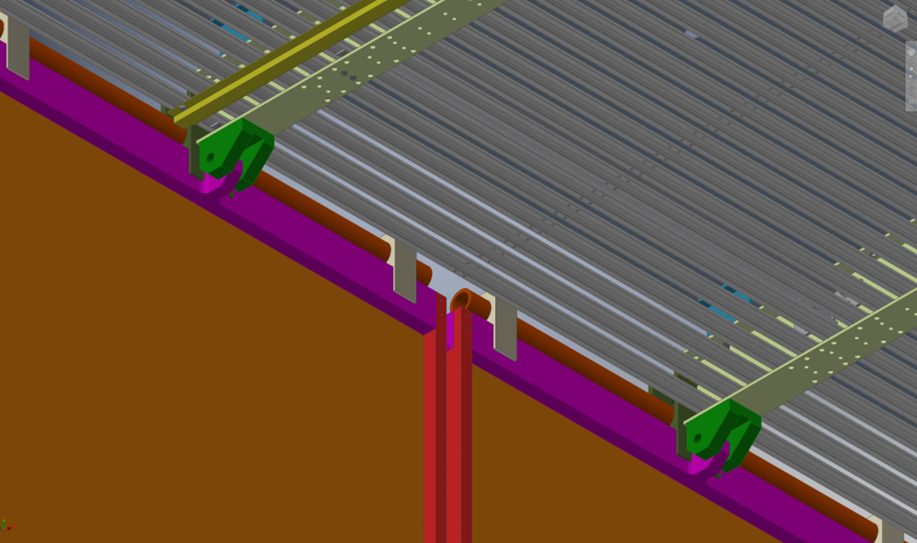
\includegraphics[width=0.8\linewidth]{tpc_fc_cpa_connection.png}
\end{cdrfigure}


%%%%%%%%%%%%
\subsubsection{FC to APA}

The I-beams of the top/bottom field cage modules are designed to be latched onto the mating brackets on the APAs.  The design details are currently being developed.   
In addition to the mechanical connection, the ground side of the divider chain must be connected to the APA's frame ground. 


%%%%%%%%%%%%
\subsubsection{FC to beam plug}
\label{subsec:fc-beamplug}
The design of the beam plug is described in Section~\ref{sec:beamplug}. In this section we describe the interface between the beam plug and the field cage. The beam plug is installed between the field cage and primary membrane where the charged particle beam enters the cryostat. Its main function is to displace about 45 cm of passive LAr layer in that region to allow the particle beam to enter the active TPC region with minimal upstream material interactions. The beam plug is mounted onto one of the field cage support structures as shown in Figures~\ref{fig:beamplug-fc} and~\ref{fig:beamplug-fc2}. The support structure is designed with sufficient  strength and stiffness to support the weight of the beam plug.
\begin{cdrfigure}[Beam plug to CPA connection]{beamplug-fc}{Beam plug to field cage interface.}
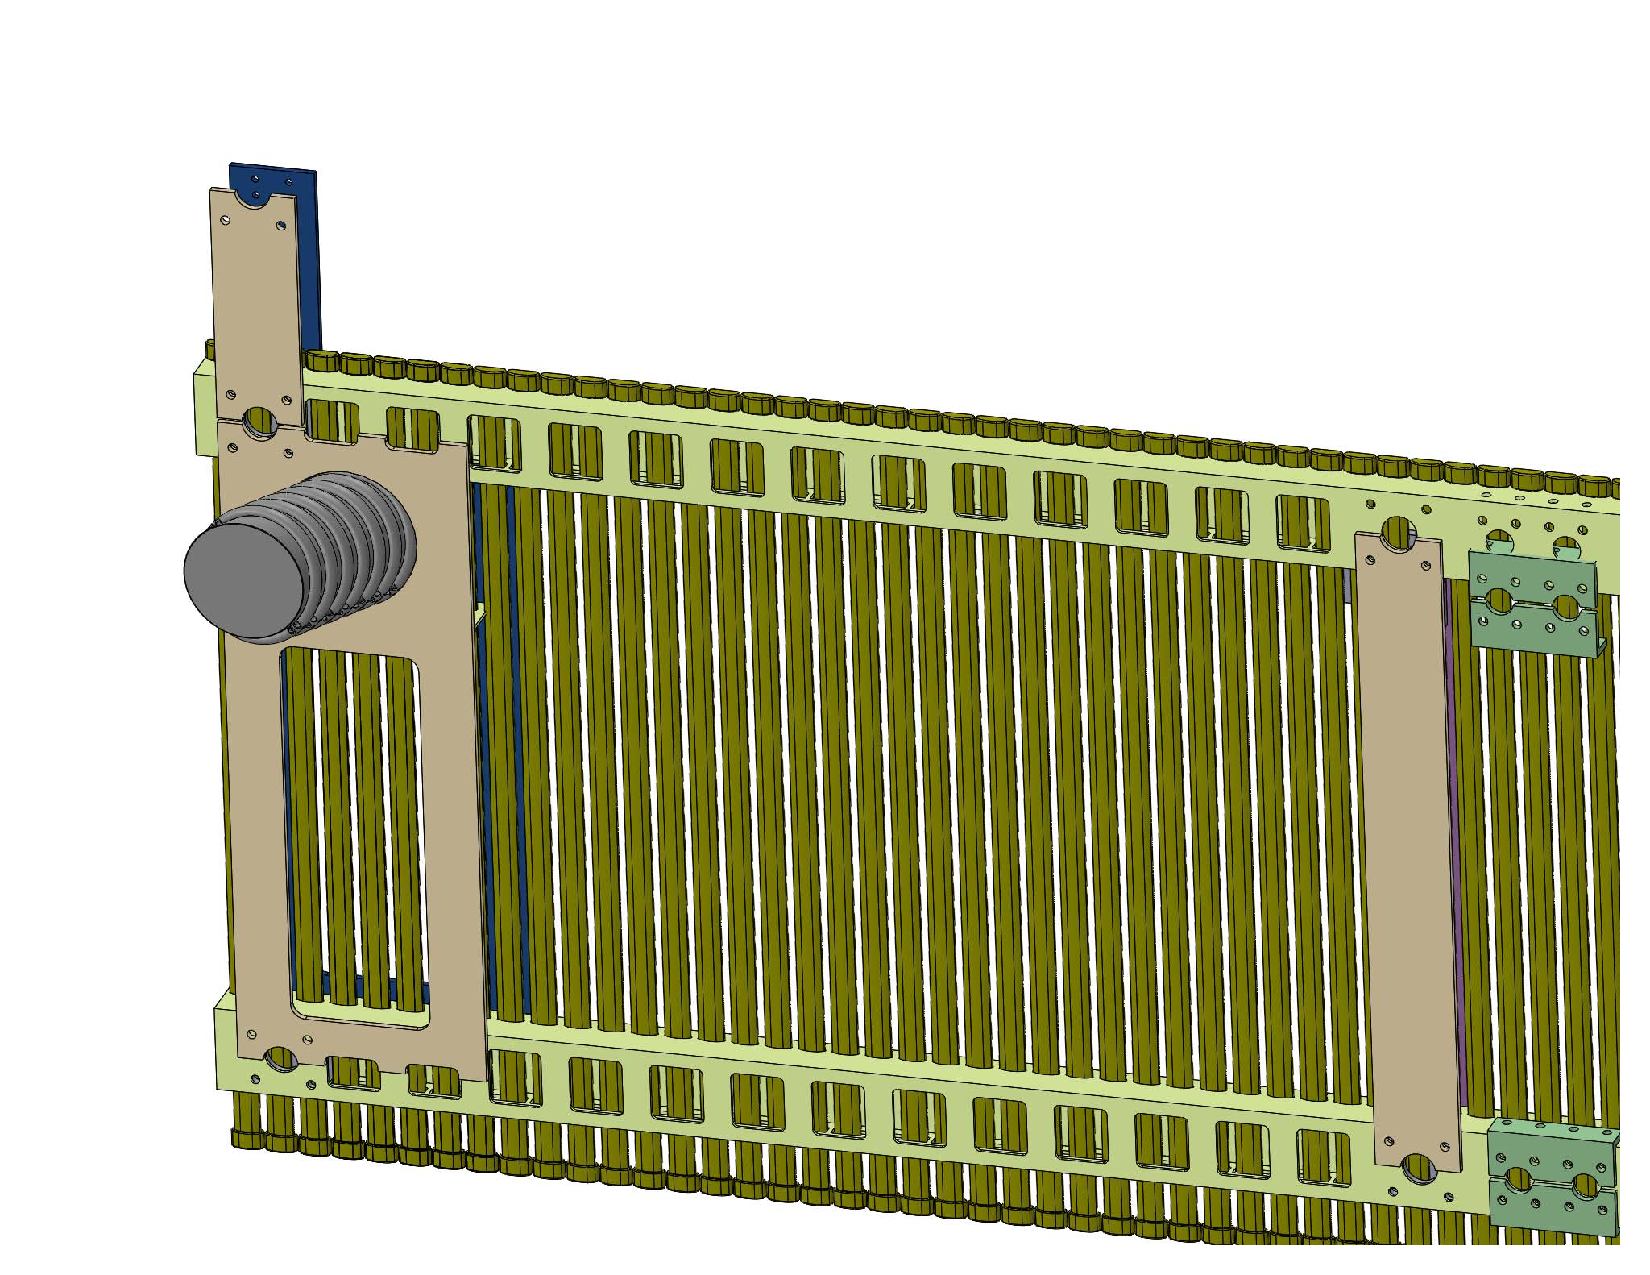
\includegraphics[width=0.75\linewidth]{beamplug-fc.pdf}
\end{cdrfigure}
\begin{cdrfigure}[Beam plug to CPA connection]{beamplug-fc2}{Cutaway sideview of the beam plug to field cage interface.}
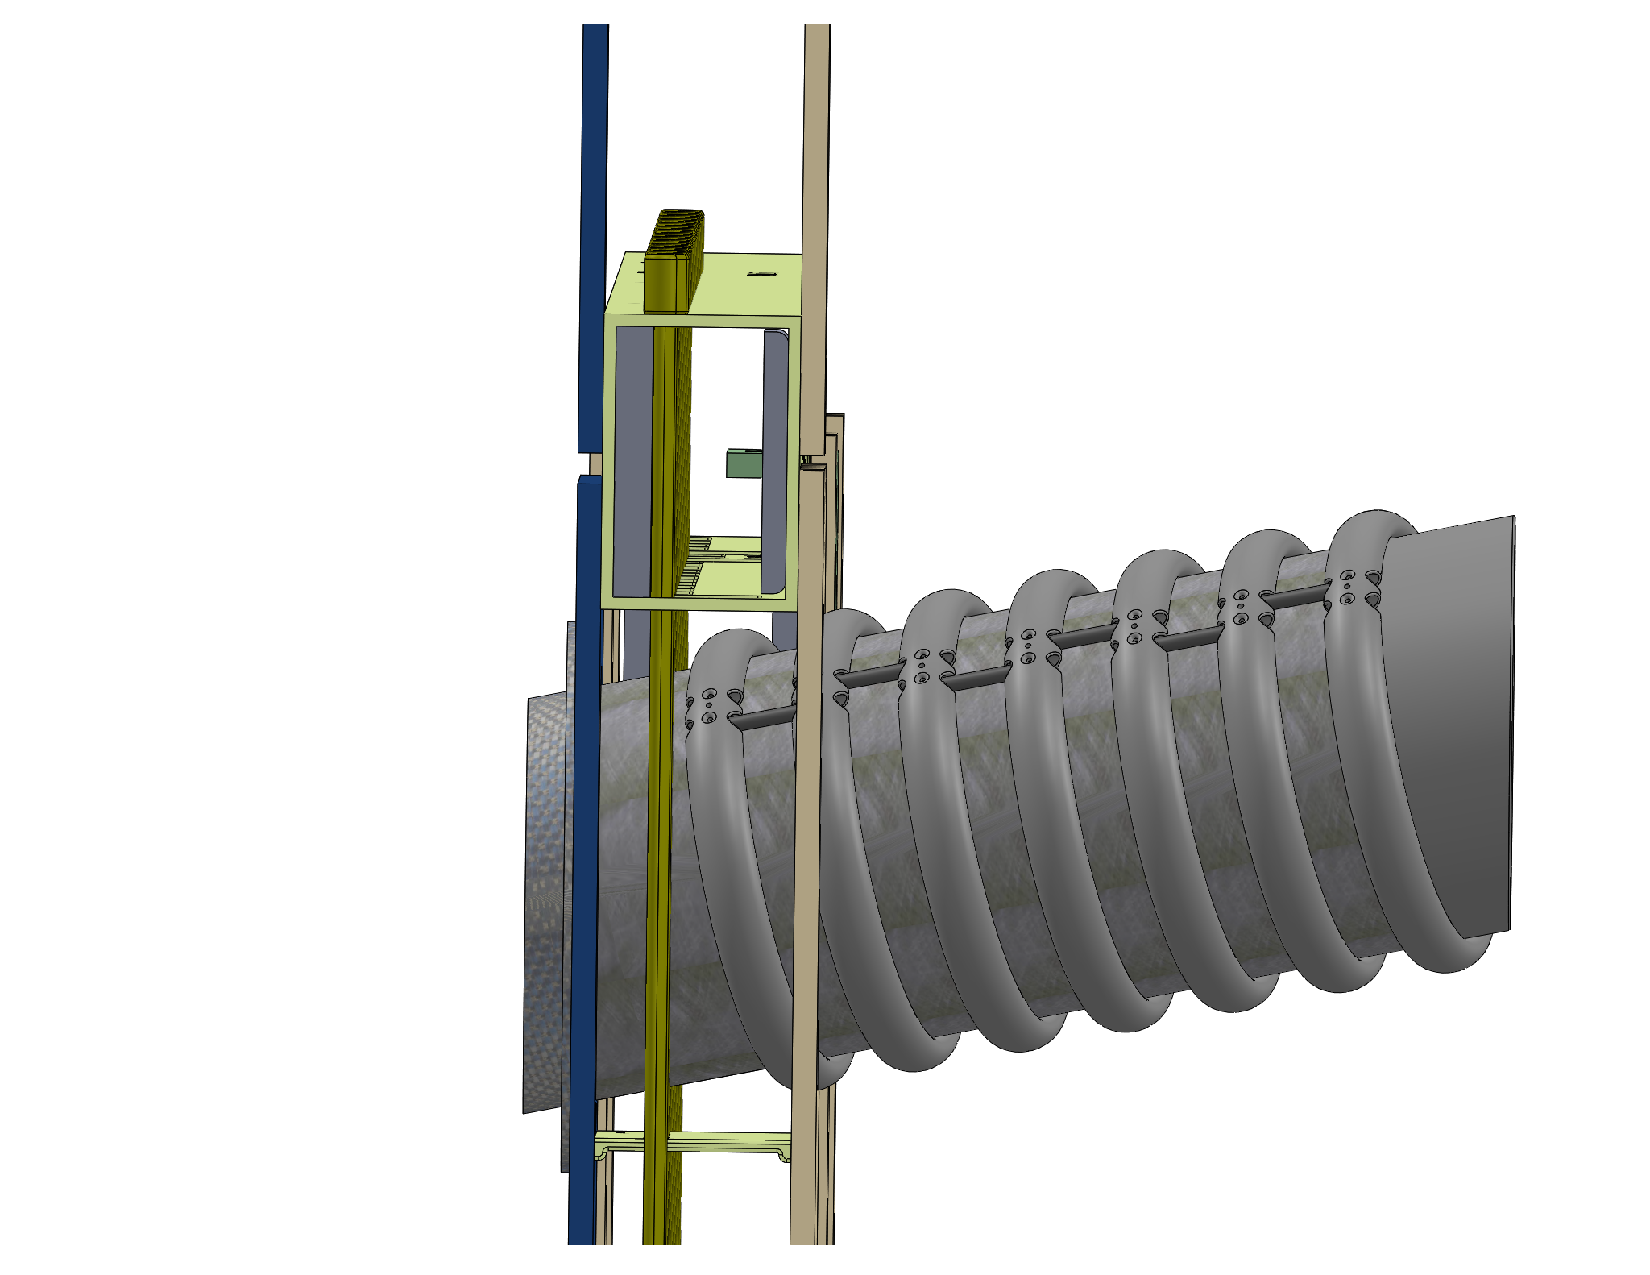
\includegraphics[width=0.5\linewidth]{beamplug-fc2.pdf}
\end{cdrfigure}







%\chapter{det-comp}


%%%%%%%%%%%%%%%%%%%%%%%%%%%%%%%%%%%%%%%%%%%%%%
%\section{Anode Plane Assemblies}

%%%%%%%%%%%%%%%%%%%%%%%%%%%%%%%%%%%%%%%%%%%%%%
%\section{Cathode Plane Assemblies}

%%%%%%%%%%%%%%%%%%%%%%%%%%%%%%%%%%%%%%%%%%%%%%
%\section{Field Cage}

%%%%%%%%%%%%%%%%%%%%%%%%%%%%%%%%%%%%%%%%%%%%%%
\section{HV components}

The TPC high voltage components include the HV power supply, cables,
filter circuit, feedthrough, attachment to the resistive cathode plane
arrays, the HV bus providing low-resistance connections between CPAs,
connections to the field cage, and devices for monitoring steady state
and transient conditions of current and voltage.

A schematic of the complete TPC HV circuit is shown in Fig.\ \ref{fig:TPCHVcircuit}.

\begin{cdrfigure}[TPC HV circuit]{TPCHVcircuit}{A schematic of the TPC high voltage circuit.}
  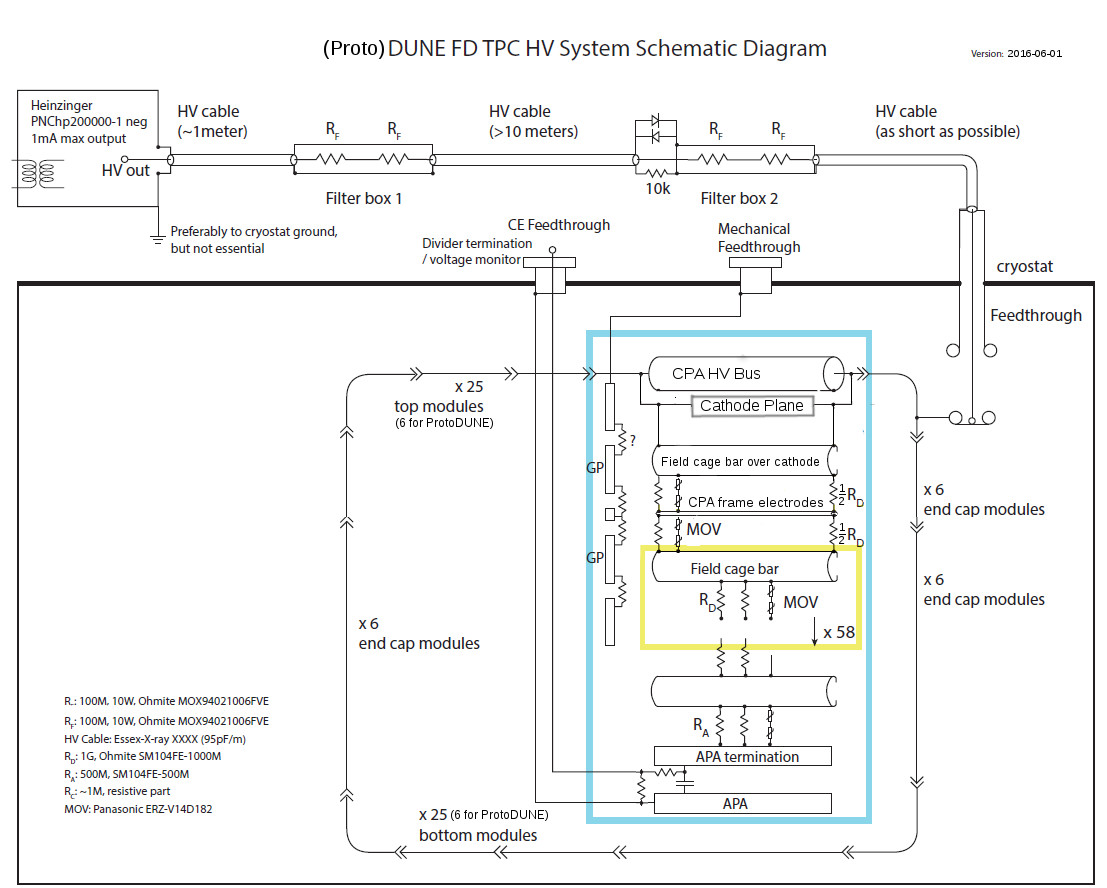
\includegraphics[width=0.75\textwidth]{VR_TPC_HV_schem-mod-1}
\end{cdrfigure}


The cathode plane will be biased at \SI{-180}{kV} to provide the
required \SI{500}{V/cm} drift field.  It will be
powered by a dedicated HV power supply through an RC filter and
feedthrough.  The power supply for the cathode plane must be able
to provide \SI{-200}{kV}.  The output voltage
ripple must not introduce more than 10\%\fixme{(?) check ripple requirement}
of the equivalent thermal
noise from the front-end electronics. The power supply must be
programmable to shut down its output at a certain current
limit. During power on and off, including output loss (for any
reason), the voltage ramp rate at the feedthrough must be controllable
to prevent damage to the in-vessel electronics from excess charge
injection. The high-voltage feedthrough must be able to withstand \SI{-250}{kV}
at their center conductors in a \SI{1}{atm} argon gas environment when
terminated in liquid argon.

%% input from F. Pietropaolo

\subsection{HV feedthrough design, Power supply, cabling}
In the present baseline option, the design of the HV feedthrough, the procurement of the Power supply and HV cables and possibly the HV filtering scheme, will take advantage of the strong synergies between Single phase and Double phase prototypes.

\begin{itemize}	
\item The Heinzinger 300 kV power supply (residual ripple less than $10^{-5}$) and the related HV cable foreseen for the DP detector are also well suited for the SP although used at lower voltage.
\item The present DP HV feedthrough design is easily adapted to the SP without any major modification in the dimensions or in the mechanical features.
\item The filtering scheme and the monitoring system is probably more demanding on the SP detector, due to the more sensitive front-end electronics, however a common development with the DP could be advantageous, allowing to get the same HV distribution chain for both the SP and the DP protoDUNE detectors.
\item Common spare components are also envisaged.
\end{itemize}

The present design of the 300 kV feedthrough is based on the very successful construction technique adopted for the ICARUS HV feedthrough, which was operated at 75 kV uninterruptedly of more that three years without any failure. The feed through was also successfully operated for several days at 150 kV.  
A coaxial geometry is adopted: the design is based on an inner conductor (HV) and an outer conductor (ground) insulated by UHMW PE  as shown in Figure~\ref{fig:hv-feed-through}. The outer conductor, made of a stainless-steel tube, surrounds the insulator extending inside the cryostat up to the LAr level. By such a geometry the electric field is always confined in regions occupied by high dielectric strength media (UHMW PE and LAr). The inner conductor is made of a thin wall stainless-steel tube, in order to minimize the heat input and to avoid the creation of argon gas bubbles around the HV lower end. A contact, welded at the upper end for the
connection to the HV cable and a round-shaped elastic contact for the connection to the cathode, screwed at the lower end, completes the inner electrode. Special care has been taken in the assembling to ensure the complete filling with the PE dielectric of the space between the inner and the outer conductors and to guarantee leak tightness at ultra-high-vacuum level.

The design of the full HV chain foreseen for the DP detector, will be finalised  after a series of tests on a prototype feed through and on the Heinzinger 300 kV Power Supply, which are presently ongoing at ETHZ and CERN. An alternative but similar design for the HV feedthrough is also under development at UCLA. Final decision on the design options will be based on max reachable HV, reliability /stability at design HV, residual noise performance.


\begin{cdrfigure}[Drawings of the HV bus.]{HVbus}{From top: A perspective view of CPA frame showing the location of the HV bus cable and attachments to the HV cup and resistive cathode (with CPA frame electrodes omitted to make HV bus visible); a sketch showing interconnection between two CPAs; a cross-section view showing equipotential lines around the HV bus and CPA frame.}
  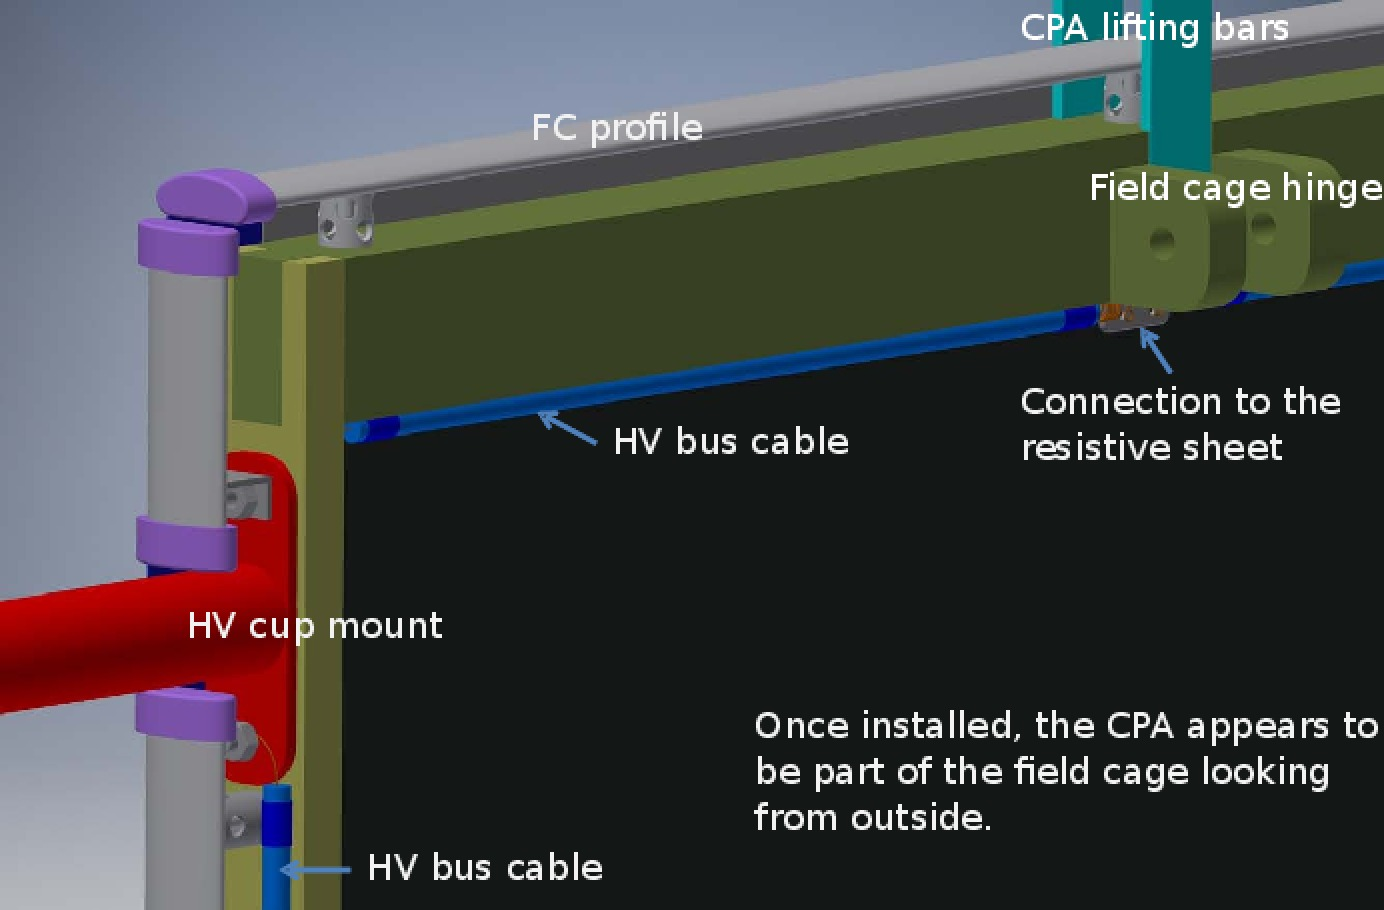
\includegraphics[height=0.29\textheight]{DUNE_SP_CPA_Design_Update-slide17-mod}
  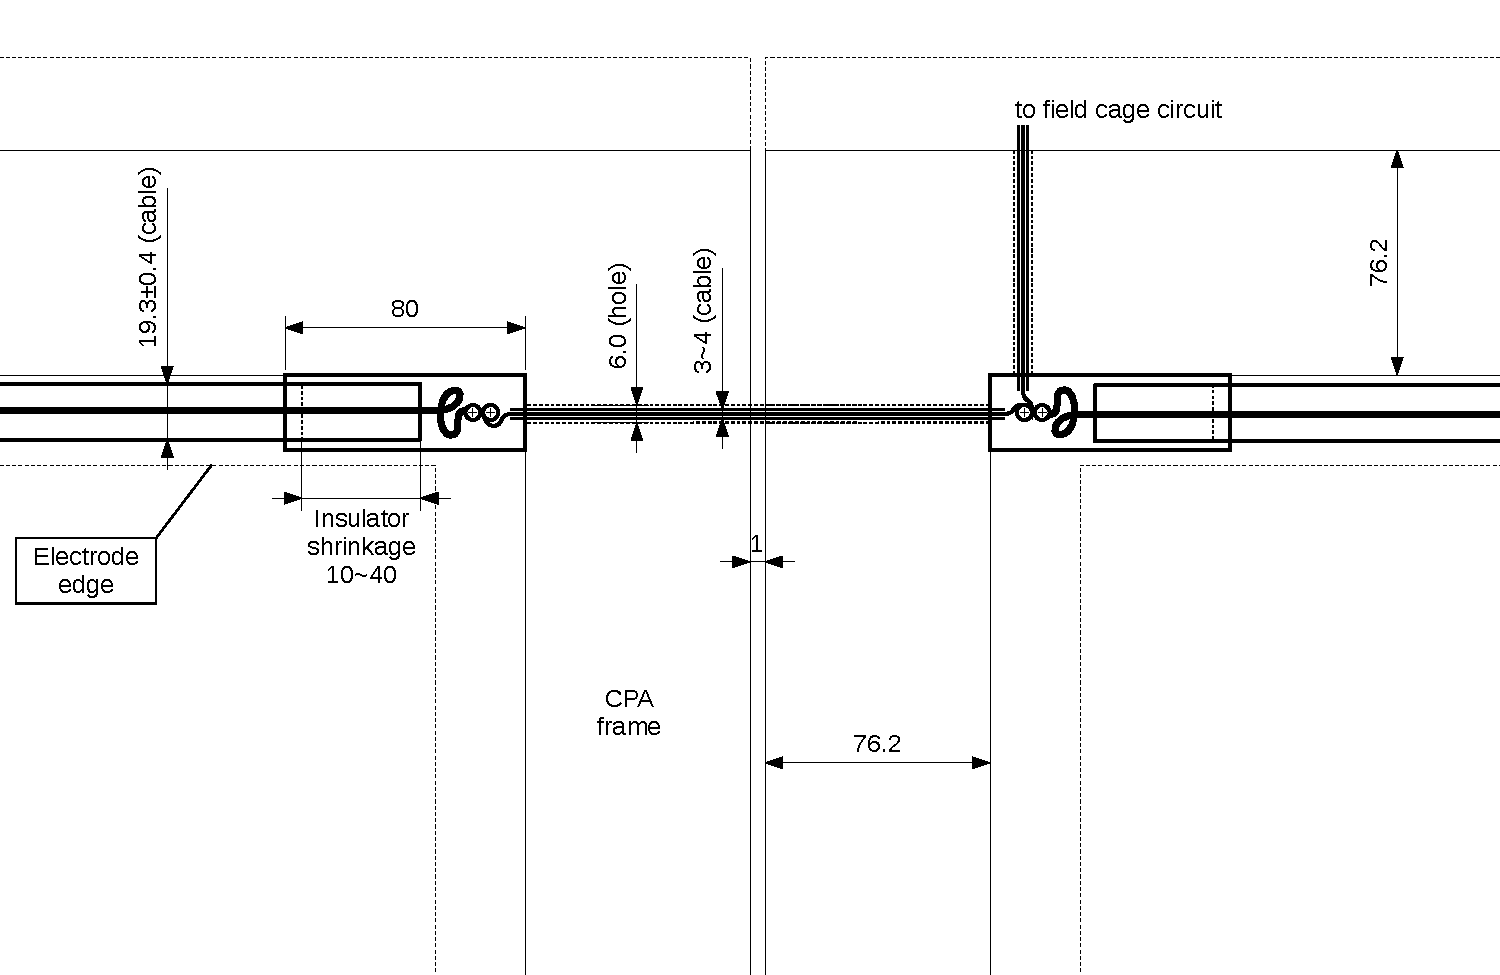
\includegraphics[height=0.3\textheight]{HVbus-connections}
  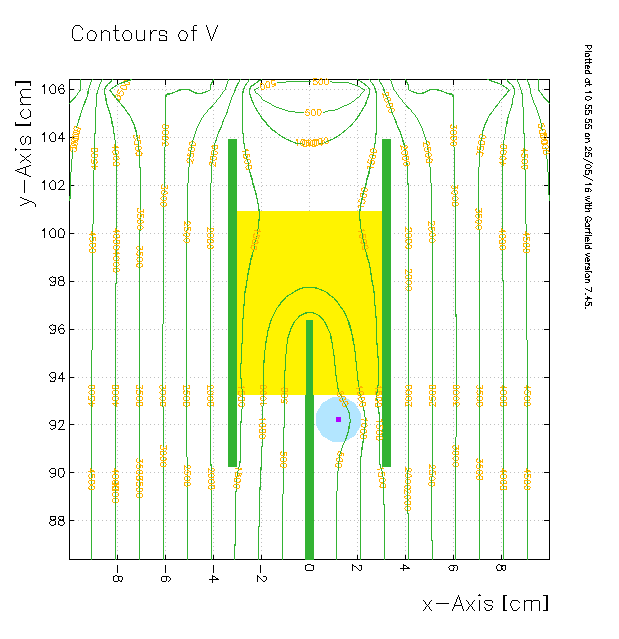
\includegraphics[height=0.3\textheight]{HVbus-vcontour}
\end{cdrfigure}

%%


Despite of the ripple spec of $10^{-5}$ from the Heinzinger power supply, the ripple amplitude is still too large for the TPC.  At 2.5m drift distance (the short drift configuration), the capacitive coupling between the cathode and the grid plane, assuming a simple parallel plate capacitor, is about 73~pF.  About 20\% of this coupling goes to the first induction plane (U).  There are 800 U wires per APA, each wire faces the CPA with half of its length. So the capacitance between a U wire and the CPA is about 18~fF.  To inject 100e noise into a U channel, it only needs about 0.9~mV of ripple on the cathode.  While the power supply at 180~kV will generate ripple voltage of 1.8~V.  Obviously for the SP TPC, further filtering of the HV output with attenuation factor of $>2000$ is needed. 

%The current candidate for the high-voltage power supplies is the 
%Heinzinger PNChp series, which has the lowest output ripple 
%specification.
Additional filtering of the voltage ripples is done
through the intrinsic HV cable capacitance and series resistors
installed inside the filter box. Established techniques and practices
will be implemented to eliminate micro-discharges and minimize
unwanted energy transfer in case of an HV breakdown.

%We have two current candidates for the feedthrough: a feedthrough
%designed by and under construction at UCLA, and the dual-phase
%feedthrough design.

As described in the CPA section above, the cathode planes will be
resistive, with electrical connections at the corners, in order to
control the energy delivered in any discharges.  A low resistance
``high voltage bus'' will provide the high voltage to the field cage
circuit and cathodes with voltage drop much less than 0.1\% of the
cathode voltage.  Field-shaping electrodes on the faces of the CPA
frames will be part of the field cage circuit, described in the field
cage section above. Field cage electrodes on the outer edges of the
CPA frames will be held at the cathode potential to provide field
uniformity and to protect the HV bus from discharge.  The feedthrough
will connect to a high voltage cup on one side of a CPA at one end of
the cathode plane.  Interconnection of the bus between CPAs will be
through HV cables passed through the CPA frames.  See
Fig.~\ref{fig:HVbus} for drawings of the high voltage bus and its
interfaces.

\begin{cdrfigure}[The HV bus.]{HVbus}{(a) Transverse cross-section of CPA top frame showing the location of the HV bus cable and equipotential contours; (b) front view showing location of cable and interconnect between two CPAs; (c) Attachment to HV cup on outer CPA frame.}
  \fixme{put in the nice figures of the HV bus}
  %\includegraphics[width=0.8\textwidth]{HVbus-figure}
\end{cdrfigure}

HV circuit monitoring devices include a toroid transformer to detect
spikes and noise in the current draw and a monitoring point at the end
of the field cage resistor chain, which also provides a means to
control field shaping around the edge of the
APA. (Fig.\ \ref{fig:TPCHVcircuit}.)

To ensure safe and reliable operation, the HV components will be
tested at a much higher voltage than expected in routine operation
($\sim\SI{250}{kV}$) in LAr. Among these tests will be a planned
``full scale'' high voltage test at Fermilab in which all components
are subjected to the full voltage and field in liquid argon in the
35-ton cryostat.



%\chapter{det-comp}


%%%%%%%%%%%%%%%%%%%%%%%%%%%%%%%%%%%%%%%%%%%%%%
%\section{Anode Plane Assemblies}

%%%%%%%%%%%%%%%%%%%%%%%%%%%%%%%%%%%%%%%%%%%%%%
%\section{Cathode Plane Assemblies}

%%%%%%%%%%%%%%%%%%%%%%%%%%%%%%%%%%%%%%%%%%%%%%
%\section{Field Cage}

%%%%%%%%%%%%%%%%%%%%%%%%%%%%%%%%%%%%%%%%%%%%%%
%\section{HV components}

%%%%%%%%%%%%%%%%%%%%%%%%%%%%%%%%%%%%%%%%%%%%%%
\section{TPC Front-end Electronics}
%\chapter{Cold Electronics}
\label{ch:ce}

%
%%%%%%%%%%%%%%%%%%%%%%%%%%%%%%%%
%\subsection{Introduction}
\subsection{Scope and requirements}
\label{subsec:ce_intro}


The DUNE single-phase TPC read-out electronics are referred to as the ``Cold Electronics'' (CE) because they reside in LAr,
mounted directly on the APA, as shown in Figure~\ref{fig:tpcce_FEMBonAPA}, thus reducing channel capacitance and noise by minimizing the length of the connection between an anode wire
and its corresponding electronics input.

\begin{cdrfigure}[The front-end electronics mounted on an APA]{tpcce_FEMBonAPA}{The 
front-end electronics as mounted on an APA.
  {\bf Top:} The front-end electronics is shown in the red circle.
  {\bf Bottom:} Cross section view. Mounting hardware between the front-end electronics 
and the APA fin is not shown.}
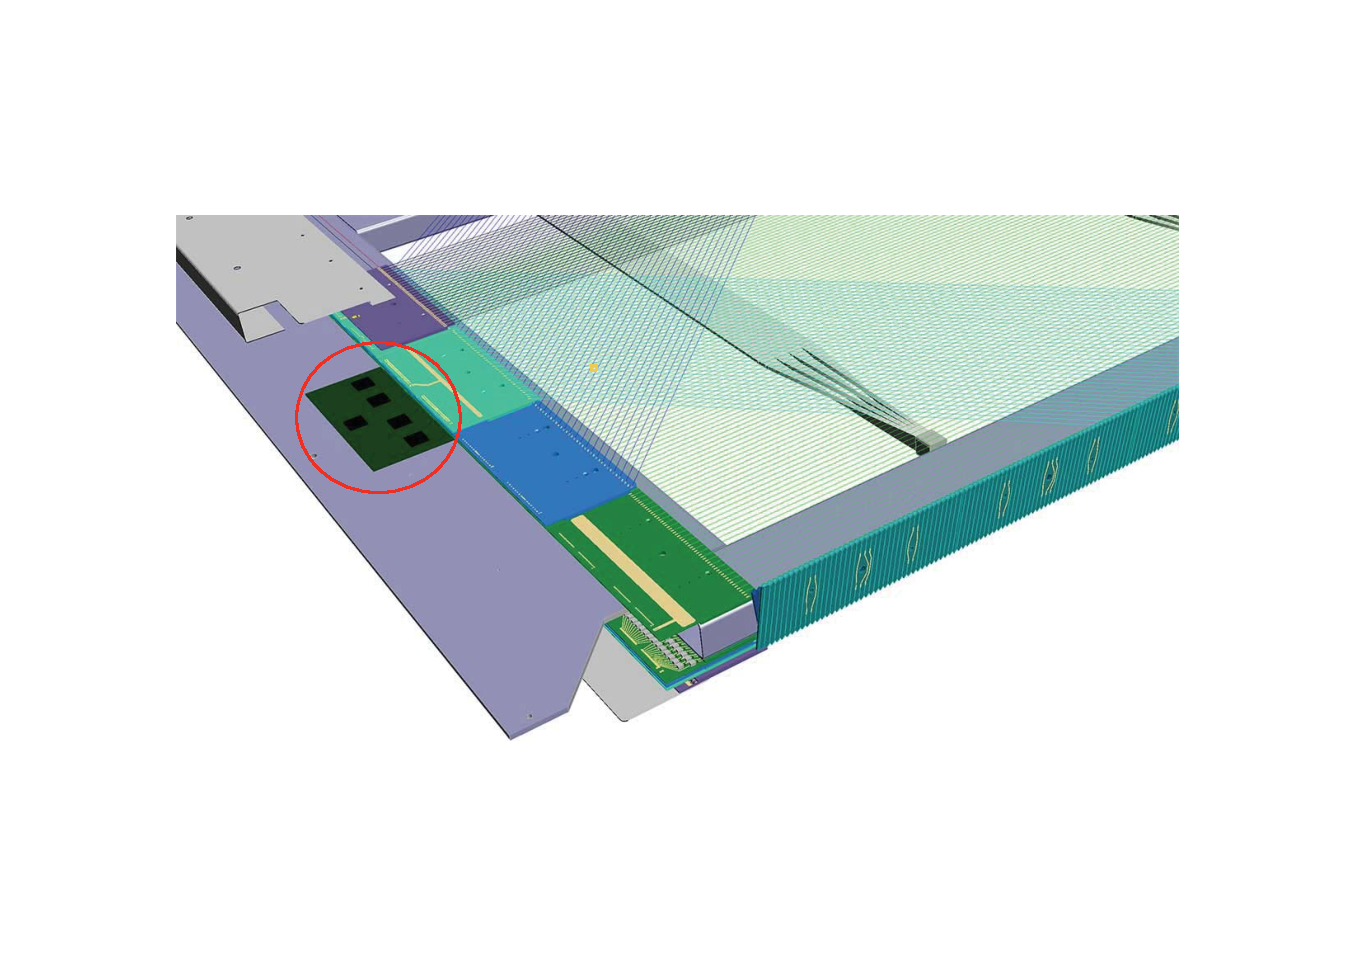
\includegraphics[width=0.8\linewidth]{tpcce_CMBonAPA_1.pdf}
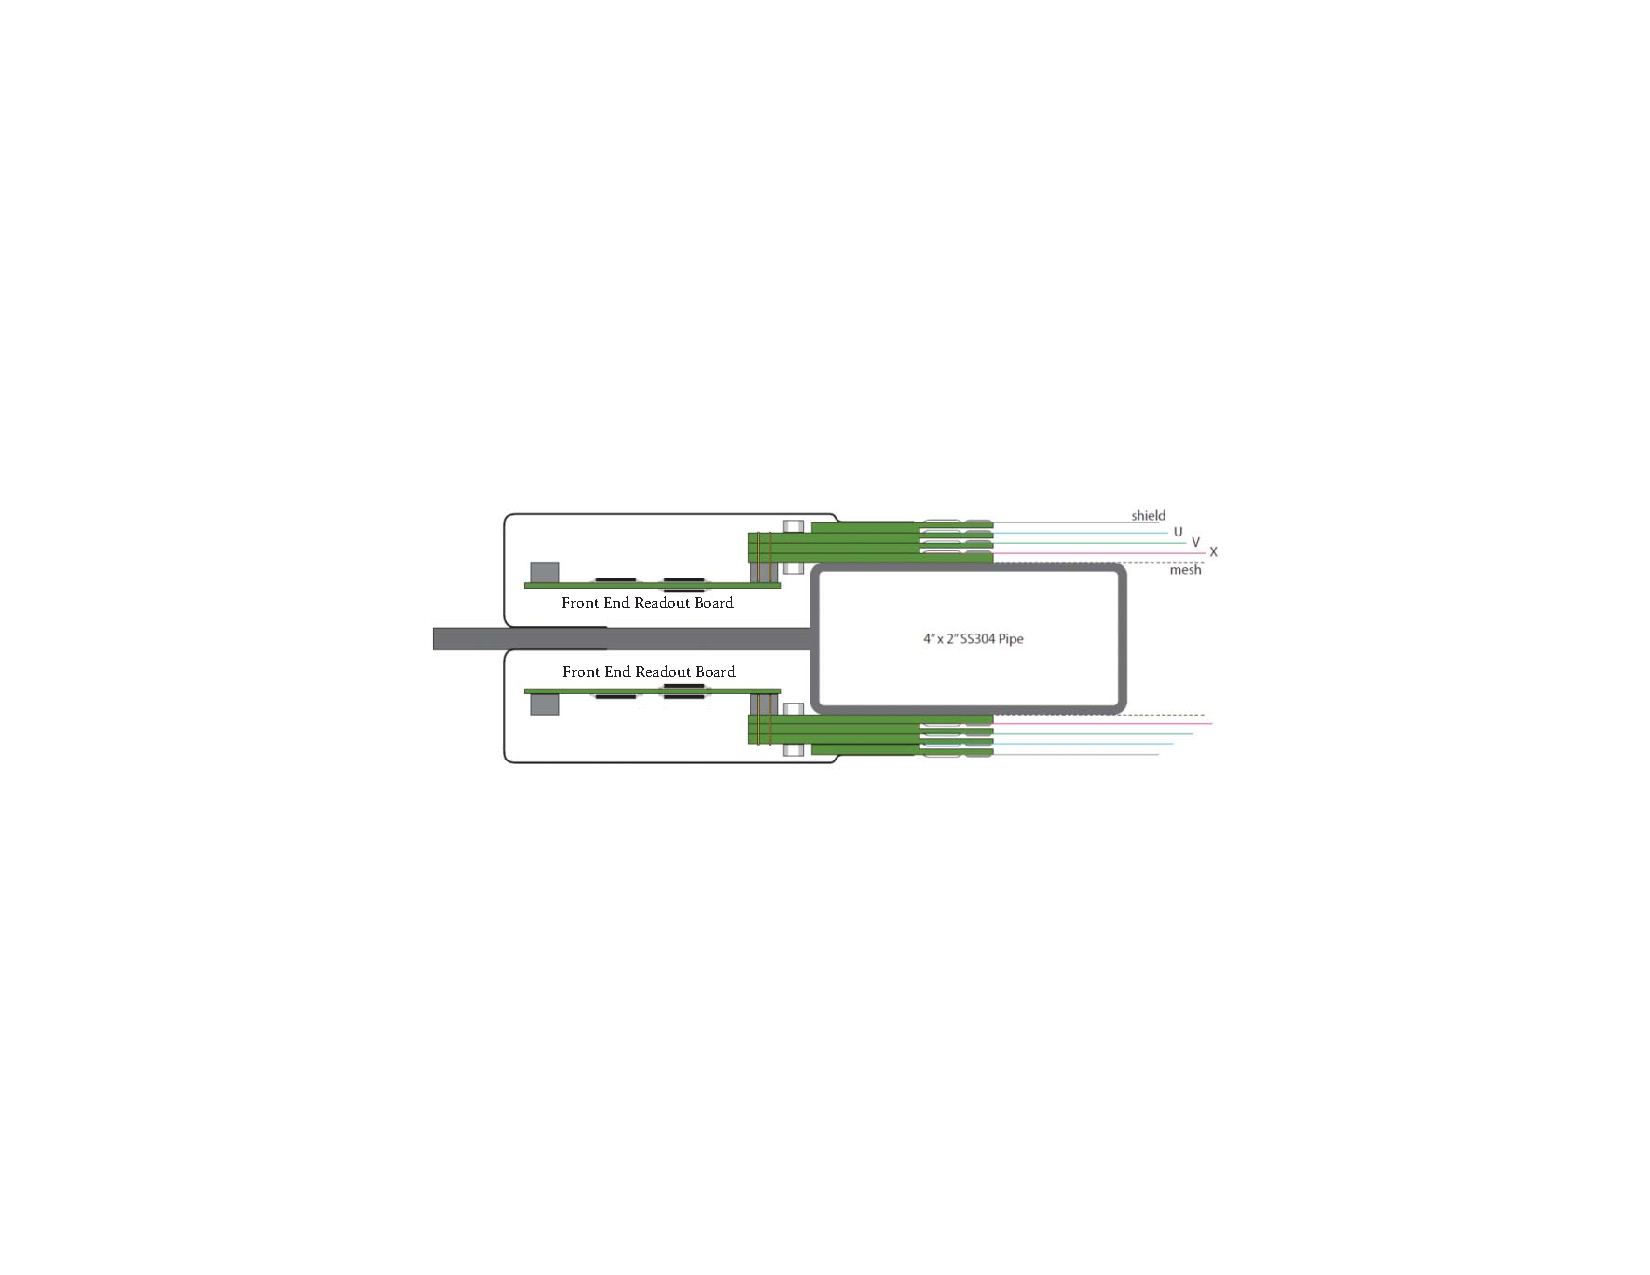
\includegraphics[width=0.8\linewidth]{tpcce_CMBonAPA_2.pdf}
\end{cdrfigure}


The CE signal processing is implemented in ASIC chips using CMOS technology,
which has been demonstrated to perform well at cryogenic temperatures,
and includes amplification, shaping, digitization, buffering, and multiplexing (MUX) of the signals.
The CE is continuously read out,
resulting in a digitized ADC sample from each APA channel (wire) up to every 500~ns (2~MHz maximum sampling rate). 

The 2,560 channels from each APA are read out by 20 Front-End Motherboards (FEMBs), each providing 
digitized wire read-out from 128 channels. One cable bundle 
connects each FEMB to the outside of the cryostat via a feedthrough (CE feedthrough) in the signal cable flange at the top of the cryostat, where a single flange services each APA, as shown in Figure~\ref{fig:tpcce_apa_flange}. 
Each cable bundle contains wires for low-voltage (LV) power, high-speed data readout,
and clock/digital-control signal distribution.
Eight separate cables carry the TPC wire-bias voltages from the signal flange to the APA wire-bias boards, as
shown schematically in Figure~\ref{fig:tpcce_cr_board}.

\begin{cdrfigure}[Connections between signal flange and APA]{tpcce_apa_flange}{Connections between
the signal flange and APA.}
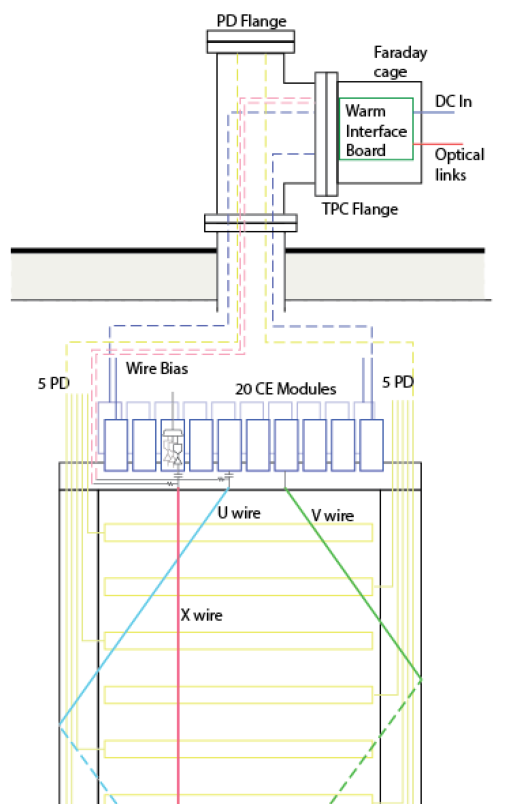
\includegraphics[width=0.4\linewidth]{tpcce_apa_flange.pdf}
\end{cdrfigure}

The components of the CE system are the
\begin{itemize}
\item Front-end mother boards (FEMBs) which house the cold ASICs and are installed on the APAs;
\item Cables for the data, clock/control signals, LV power, and wire-bias voltages 
between the APA and the signal flanges (cold cables);
\item Signal flanges with a CE feedthrough to pass the data, clock/control signals, 
LV power, and APA wire-bias voltages between the inside and outside of the cryostat;
\item Warm electronics crates (WECs) that are mounted on the signal flanges and contain the Warm Interface Boards (WIBs)
and Power and Timing Cards (PTCs) for further processing and distribution of the signals entering/exiting the cryostat;
\item Fiber cables for transmitting data and clock/control signals between the WECs and the data acquisition 
(DAQ) and slow control systems;
\item Cables for LV power and wire-bias voltages between the signal flange and external power supplies (warm cables);
\item LV power supplies for the CE and bias-voltage power supplies for the APAs
\end{itemize}

The electrical cables for each APA enter the cryostat through a single 
signal flange, creating an integrated unit that provides local diagnostics for noise and validation testing,
and follows the grounding guidelines in Section~\ref{subsec:groundshield}. The components, the quantity of each required for ProtoDUNE-SP, and the number of channels that each component has, are listed in Table~\ref{tab:ce-components}.

\begin{cdrtable}[Electronics components and quantities]{llr}{ce-components}{Electronics components and quantities}
Element                                                             &  Quantity                                  &  Channels per element   \\  \toprowrule
TPC                                                                   & 1                                               & 15,360    \\  \colhline
APA                                                                   & 6                                               & 2,560     \\  \colhline
Front-End Mother Board (FEMB)                         & 120, 20 per APA                       & 128     \\  \colhline
%\hspace{0.02\textwidth} 
FE ASIC chip                                & 120 $\times$ 8, 8 per FEMB      & 16          \\   \colhline
ADC ASIC chip                             & 120 $\times$ 8, 8 per FEMB      & 16          \\   \colhline
FEMB FPGA                                  & 120, 1 per FEMB                         & 128          \\   \colhline
Cold cable bundles                                           & 120, 1 per FEMB                        & 128      \\   \colhline
Signal flange                                                     & 6, 1 per APA                              & 128 $\times$ 20  (i.e., 2,560)      \\   \colhline
CE feedthrough                            & 6, 1 per APA                             &128 $\times$ 20         \\   \colhline
Warm interface boards (WIB)         & 30, 5 per APA                             & (128 $\times$ 20) /5 (i.e., 512)        \\   \colhline
 Warm electronics plates (WEC)      & 6, 1 per APA                             & 128 $\times$ 20         \\   \colhline
 Power and timing cards (PTC)       & 6, 1 per APA                             & 128 $\times$ 20         \\   \colhline
Passive backplane (PTB)                & 2                                              &   ?? \\   \colhline
MPOD  power supplies (chassis???)                     & 2, 1 per 3 APAs                        &   \SI{15360}/2   \\  
\end{cdrtable}

\fixme{check Table~\ref{tab:ce-components} ; there are some missing numbers}


The most significant requirements for the CE are listed here. The CE shall:

\begin{itemize}	
\item Provide the means to read out the TPC wires and transmit their data in a useful format to the DAQ.
\item Operate for the life of the facility without significant loss of function.
\item Record the channel waveforms continuously without dead time.
\item Be constructed only from materials that are compatible with high-purity LAr.
\item Provide sufficient precision and range in the digitization to:
\begin{itemize}
\item Discriminate electrons from photon conversions;
\item Optimize the reconstruction of high- and low-energy tracks from accelerator-neutrino interactions;
\item Distinguish a Minimum Ionizing Particle (MIP) from noise with a signal-to-noise ratio $>$ 9:1;
\item Measure  ionization up to 15 times that of a MIP particle, so that stopping kaons from proton decay can be identified.
\end{itemize}
\item Ensure that all power supplies have: 
\begin{itemize}
\item Local monitoring and control
\item Remote monitoring and control through DAQ
\item Over-current and over-voltage protection circuits
\end{itemize}
\item Ensure that the CE feedthroughs are able to withstand twice their nominal operating voltages 
with a maximum specified leakage current in 1-atm argon gas.
\end{itemize}


%%%%%%%%%%%%%%%%%%%%%%%%%%%%%%%%
\subsection{Grounding and shielding}
\label{subsec:groundshield}

To avoid structural ground loops, the APA frames described in Section~\ref{subsec:apa_frame} 
are insulated from each other. Each frame is electrically connected to the cryostat at a single 
point on the CE feedthrough board in the signal flange where the cables exit the cryostat. Mechanical suspension of the APAs 
is accomplished using insulated supports. 

The analog portion of the FEMB contains eight front-end (FE) ASICS configured as 16-channel 
digitizing charge amplifiers. Input amplifiers on the ASICs have their Common terminals connected 
to the APA frame.  All power-return leads and cable shields 
are connected to both the Common plane of the FEMB and to the signal flange.

Filtering circuits for the APA wire-bias voltages are locally referenced to the Common plane of the FEMBs through low-impedance 
electrical connections. This approach ensures a ground-return path in close proximity to the 
bias-voltage and signal paths. The close proximity of the current paths minimizes the size of potential loops to further 
suppress noise pickup.

Photon detector signals, described in Section~\ref{sec:pd_system}, are carried directly on shielded, 
twisted-pair cables to the signal flange. The cable shields are connected to the 
cryostat at a second feedthrough, the PDS feedthrough, and to the PCB shield layer on the photon detectors \fixme{readout boards?}. There is no 
electrical connection between the cable shields and the APA frame except at the signal flange.

%
%%%%%%%%%%%%%%%%%%%%%%%%%%%%%%%%
\subsection{Distribution of APA wire-bias voltages}
\label{subsec:ce_wire_bias}

Each side of an APA includes four wire layers as described in Section~\ref{subsec:apa_phys_desc}. 
The inner-most X-plane layer of wires is nominally biased at +820 Volts, with each wire AC coupled 
to one of the 128 charge amplifier circuits on the FEMB. The V-plane wire layer is effectively biased at zero volts, 
with each wire directly connected to one of the charge amplifier circuits. The U-plane wire layer is nominally 
biased at $-$370 Volts with each wire AC-coupled 
to one of the 128 charge amplifier circuits. The outermost G-plane wire layer,
which has no connection to the charge amplifier circuits, is biased at $-$665 Volts.

Electrons passing through the wire grid must drift unimpeded until they reach the X-plane 
collection layer. The nominal bias voltages are predicted to result in this electrically 
transparent configuration.

As described in Section~\ref{subsec:apa_phys_desc}
\fixme{right section reference?}
 the filtering of wire-bias voltages and AC coupling of wire signals passing
onto the charge amplifier circuits is done on  CR boards that plug inbetween the APA wire-board stacks and FEMBs.

Each CR board includes single R-C filters for the X- and U-plane wire-bias voltages. In addition, each board has 48 
pairs of bias resistors and AC coupling capacitors for X-plane wires, and 40 pairs for the U-plane wires. The coupling capacitors block DC while passing AC 
signals to the CE motherboards.

\begin{cdrfigure}[APA wire bias schematic diagram]{tpcce_cr_board}{APA wire bias 
schematic diagram, including the Capacitance-Resistance (CR) board.}
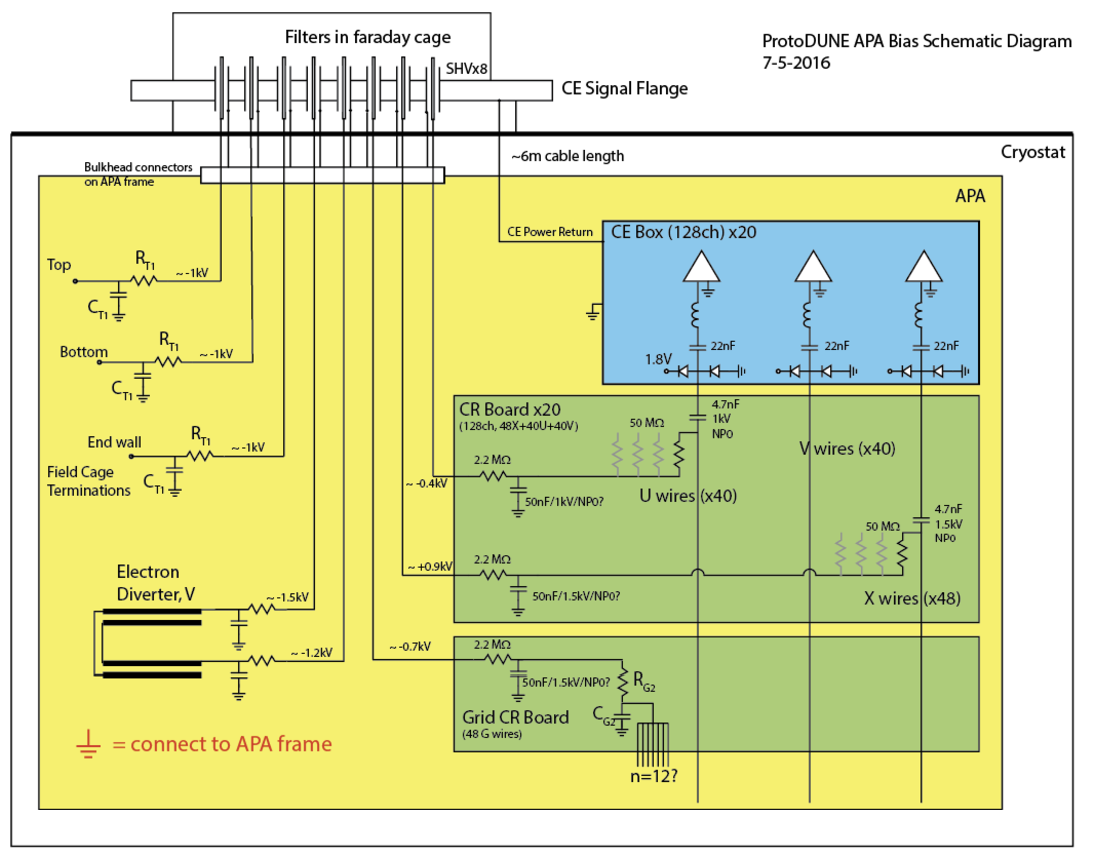
\includegraphics[width=0.9\linewidth]{tpcce_cr_board.pdf}
\end{cdrfigure}

Separate CR boards include a single R-C filter for the G-plane wires and 12 pairs of bias resistors and
coupling capacitors.
Groups of four wires are tied together to share single
bias resistors and filter capacitors. These CR boards do not connect to the charge amplifier circuits on the FEMB.

The amplifier circuits 
have input impedance of 50~$\Omega$ using 22-nF coupling capacitors. 
Clamping diodes limit the input voltage received at the amplifier circuits to between zero and +1.8 Volts.


Coupling capacitors for the X-plane and U-plane wires are required to block DC bias voltages.
However they also impact the efficiency of the detector circuits.
The sense wires are expected to have 200 pF of capacitance to the APA frame.
Induced or collected charges are effectively divided between the wire capacitance and the coupling capacitor.
To achieve a charge-calibration accuracy of 0.5 percent or better,
the coupling capacitors must be 4.7 nF at ten percent tolerance, or 2.2 nF at five percent tolerance.
Voltage ratings should be at least 1.5 times the expected operating voltages.

Bias resistance values should be at least 20 Meg-ohms to maintain negligible noise contributions.
A target value of 50 Meg-ohms is desired.
The higher value helps to achieve a longer time constant for the high-pass coupling networks.
Time constants should be at least 25 times the electron drift time so that the undershoot in the digitized waveform
is small and easily correctable.
However, leakage currents can develop on PC boards that are exposed to high voltages over extended periods.
If the bias resistors are much greater than 50 Meg-ohms, leakage currents may affect the bias voltages applied to the wires.

The bias-voltage filters are R-C low-pass networks.
Resistance values should be much smaller than the bias resistances to control crosstalk between wires
and limit the voltage drop if any of the wires becomes shorted to the APA frame.
A value around 2.2 Meg-ohms is desired.
Smaller values may be considered although a larger filter capacitor would be required to maintain a given level of noise reduction.
A target value of 47 nF has been established for the filter capacitors.

For the grid-plane bias filters, component values are less critical.
If possible they will be identical to those used for the bias resistors and coupling capacitors
(50~M$\Omega$ and 2.2 to 4.7~nF).


%%%%%%%%%%%%%%%%%%%%%%%%%%%%%%%%
\subsection{Front-End Mother Board}
\label{subsec:fe_arch}

The main component of the CE architecture illustrated in Figure~\ref{fig:tpcce_schem} is the 
128-channel FEMB, which itself consists of an analog motherboard and an attached FPGA 
mezzanine card for processing the digital outputs.
Each APA is instrumented with 20 FEMBs, for a total of 2,560 channels per APA.
The FEMBs plug directly into the APA CR boards, making the connections from the U- and V-plane induction wires and 
X-plane collection wires to the charge amplifier circuits as short as possible.

The analog mother board is instrumented with eight 16-channel FE ASICs,
eight 16-channel ADC ASICs, LV power regulators, and input-signal protection circuits.
The 16-channel FE ASIC provides amplification and pulse shaping.
The 16-channel ADC ASIC comprises  12-bit digitizers performant at speeds up to 2 MS/s, local buffering,
and an 8:1 MUX stage with two pairs of serial readout lines in parallel.

 
   (Figure~\ref{fig:tpcce_CMBpix}).
% following pgraph moved up 9/27   
Each FE ASIC channel has a charge amplifier circuit with a gain selectable from one of 4.7, 7.8, 14 and 25~mV/fC
(full scale charge of 55, 100, 180 and 300~fC),
a high-order anti-aliasing filter with adjustable time
constant (peaking time 0.5, 1, 2, and 3 $\mathrm{\mu}$s),
an option to enable AC coupling,
and a baseline adjustment for operation with either the collecting (200~mV) or the non-collecting (900~mV) wires.
Shared among the 16 channels in the FE ASIC are the bias circuits, programming registers,
a temperature monitor, an analog buffer for signal monitoring, and the digital interface.
The estimated power dissipation of FE ASIC is about 6~mW per channel at 1.8~V supply.

The FE ASIC layout is shown in Figure~\ref{fig:tpcce_ADC_ASIC}.
The ASIC was implemented using the commercial CMOS process (0.18~$\mu$m and 1.8~V), which 
is expected to be available for at least another 10~years. 
The charge amplifier input MOSFET is a p-channel biased at 2~mA with a L/W (channel length/width) ratio
of 0.27~$\mu$m / 10~$\mu$m, followed by dual cascade stages.
The charge amplification and shaping filter have digitally programmable gain and peaking time
(as specified in Section~\ref{subsec:fe_arch}).
Each channel also implements a high-performance output driver,
which can be used to drive a long cable, but is disabled when interfaced to an ADC ASIC to reduce the power consumption.
The ASIC integrates a band-gap reference (BGR) to generate all the internal bias voltages and currents.
This guarantees a high stability of the operating point over a wide range of
temperatures, including cryogenic.
The ASIC is packaged in a commercial, fully encapsulated plastic QFP 80 package.

Prototypes have been evaluated and characterized at RT (300~K) and LN2 (77~K) temperature.
During testing the circuits have been cycled multiple times
between the two temperatures and operated without any change in performance.
Figure~\ref{fig:tpcce_shaper_out} shows the measured pulse response, both as a function
of temperature and the programmable settings of the chip.
These results are in close agreement with simulations and indicate
that both the analog and the digital circuits and interface operate as
expected in a cryogenic environment.

\begin{cdrfigure}[Measured pulse response with details]{tpcce_shaper_out}{Measured pulse response with
 details on gain, peaking time and baseline adjustments}
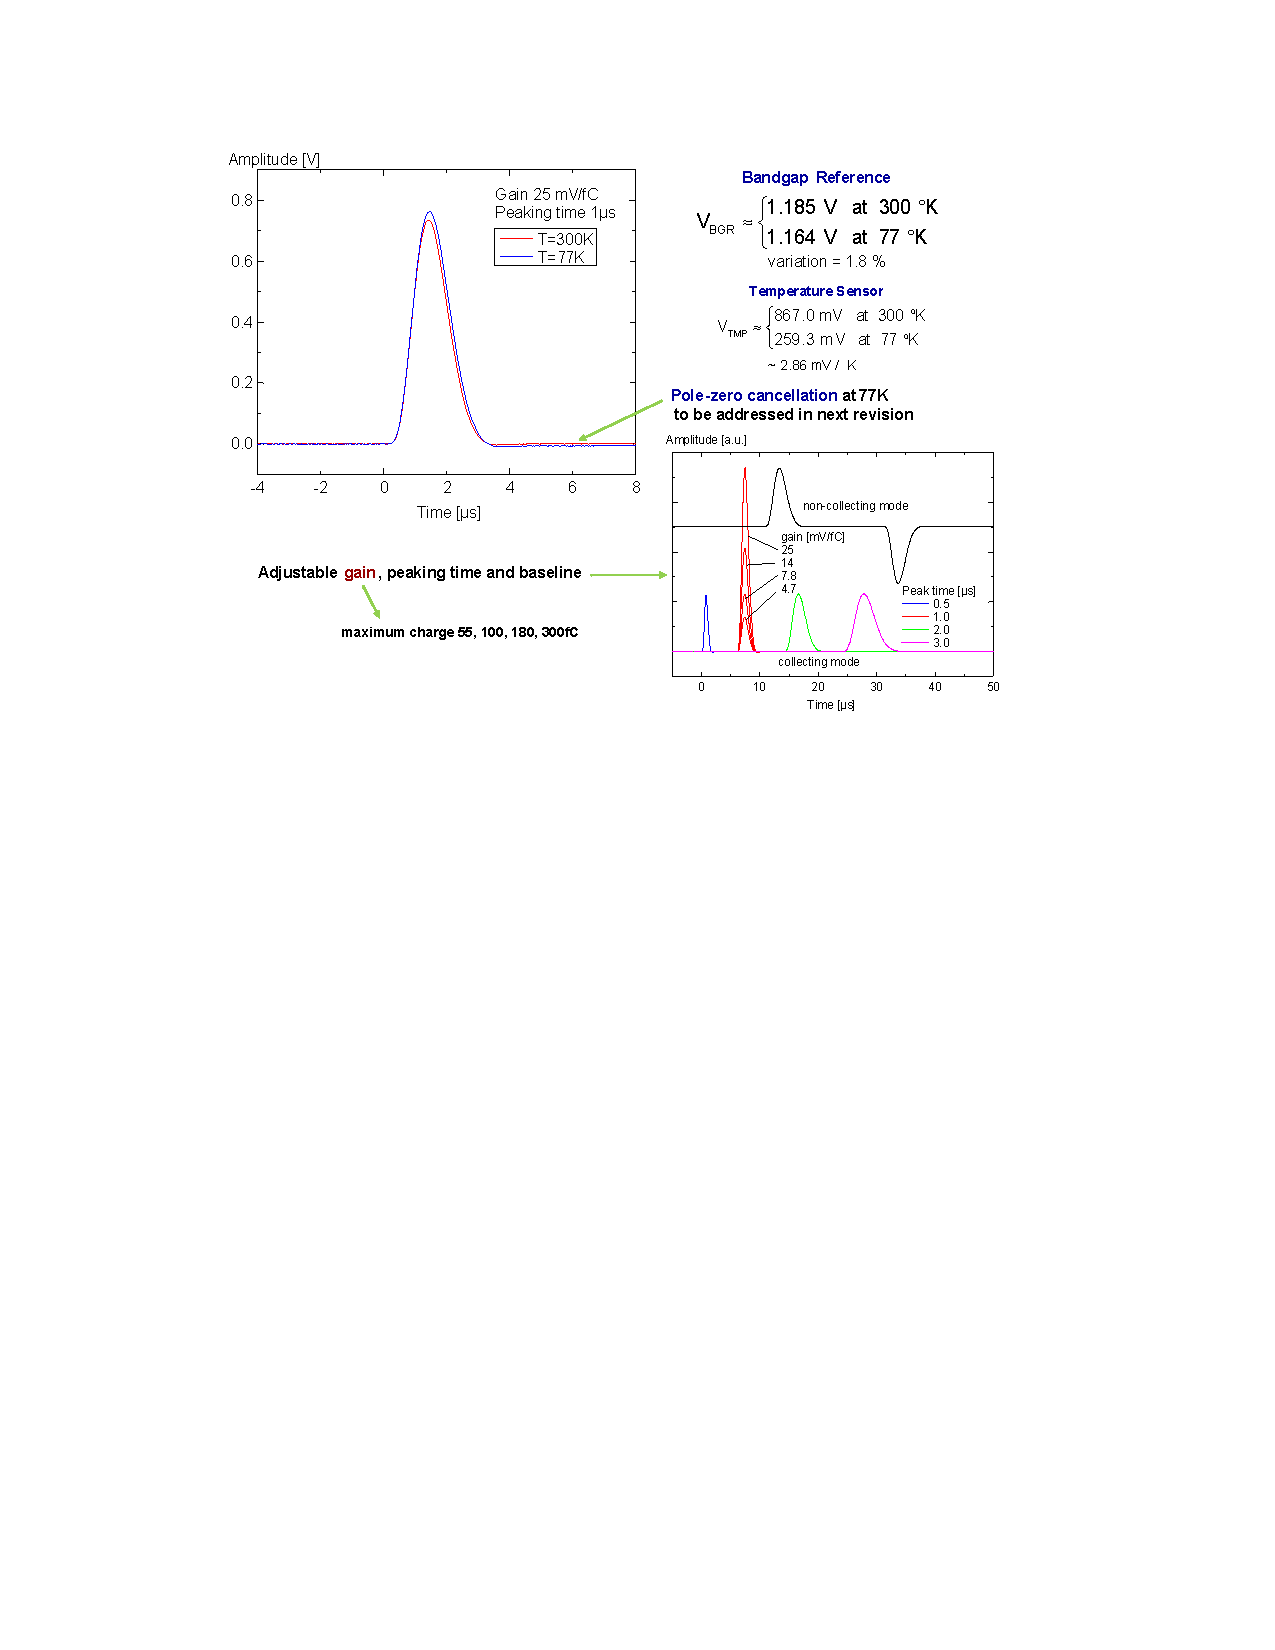
\includegraphics[width=\linewidth]{tpcce_shaper_out.pdf}
\end{cdrfigure}

\begin{cdrfigure}[Measured ENC vs filter time constant]{tpcce_enc}{
Measured ENC vs filter time constant from the latest prototype version of the FEMB
for two different gains, 14~mV/fC and 25~mV/fC. RT = room temperature and 
LN2 = liquid nitrogen}
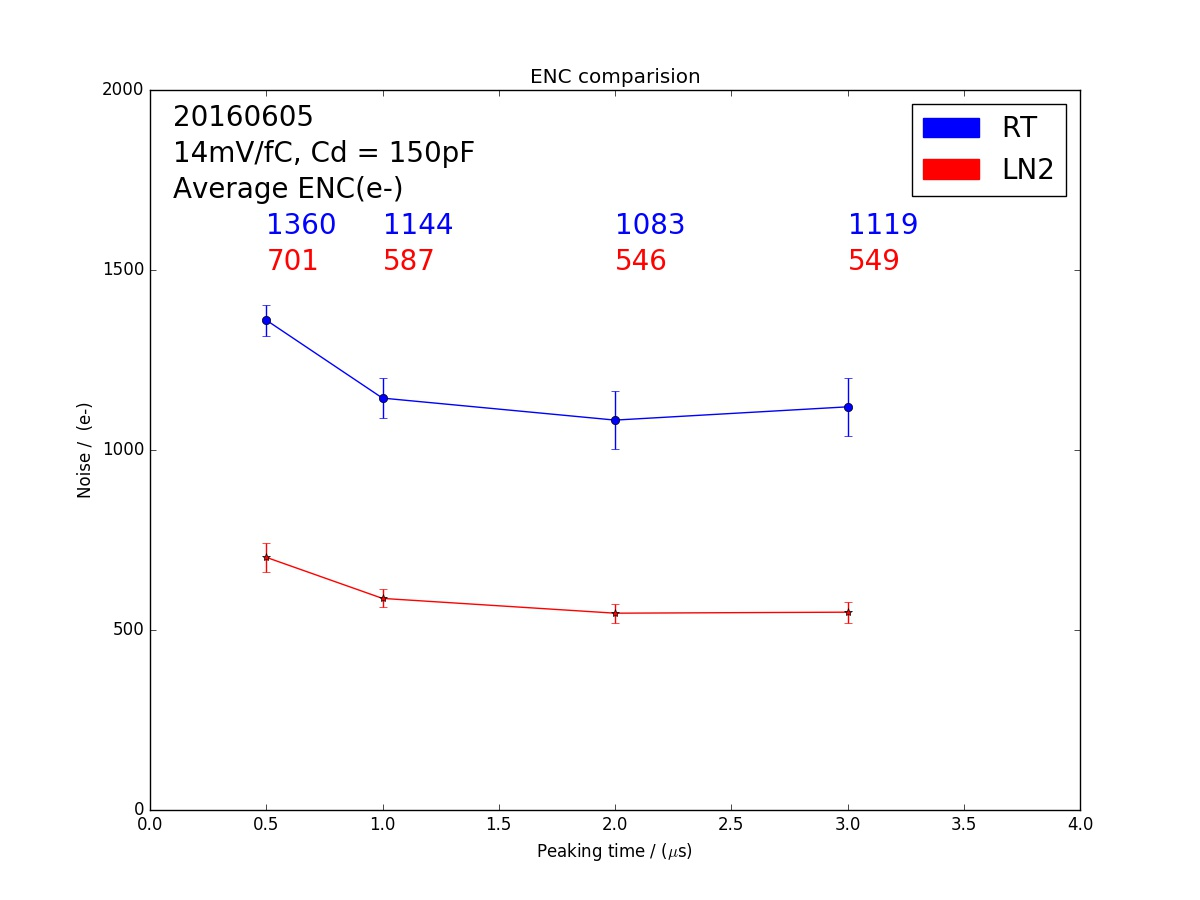
\includegraphics[width=0.45\linewidth]{tpcce_enc_14mV.jpg}
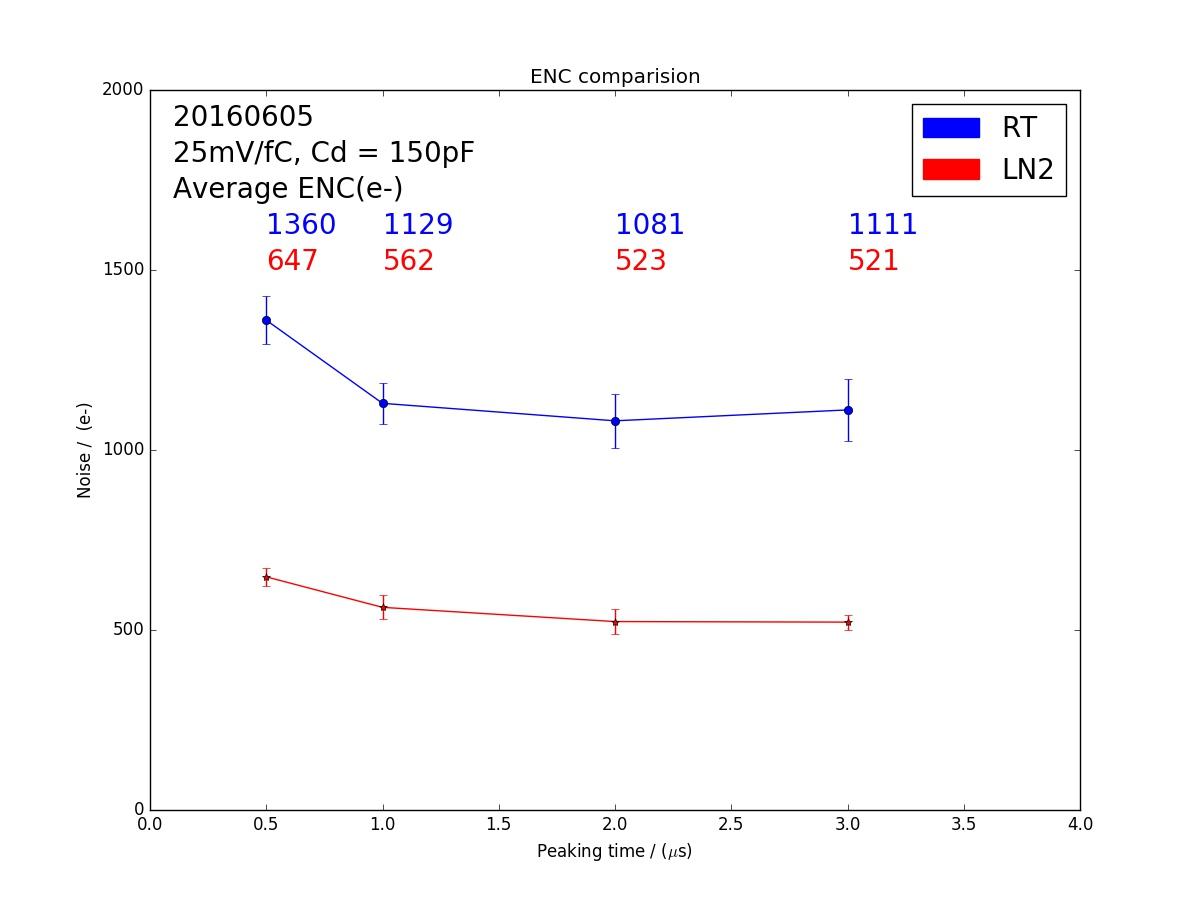
\includegraphics[width=0.45\linewidth]{tpcce_enc_25mV.jpg}
\end{cdrfigure}

Figure~\ref{fig:tpcce_enc} shows the measured Equivalent Noise Charge (ENC) versus 
filter-time constant (peaking time) for two different gains, where ENC is the value of charge 
(in electrons) injected across the detector capacitance that would produce at the output of the 
shaping amplifier a signal whose amplitude equals the output R.M.S. noise. These measurments
were made with prototype FEMBs at both RT and submerged in LN2 with a wire-simulating input capacitance of $C_f~=~150$~pF.
In LN2, for peaking times $>$1~$\mu$s, less than 600~e$^{-}$ was measured. For comparison,
a MIP travelling perpendicularly to the wire plane in the direction of wire spacing is
expected to deposit $\sim$~10,000~e$^{-}$ on the collection wires, for a worst-case
S:N$\sim$16:1.

Each channel is equipped with an injection capacitor which can be used
for test and calibration and can be enabled or disabled through a
dedicated register. The injection capacitance has been measured using 
a calibrated external capacitor. The measurements show
that the calibration capacitance is extremely stable, changing from
184~fF at RT to 183~fF at 77~K. This result and the measured
stability of the peaking time demonstrate the high stability of the
passive components as a function of temperature. Channel-to-channel and chip-to-chip
variation in the calibration capacitor are typically less than 1\%. 

The ADC ASIC design is also implementd using the CMOS process (0.18~$\mu$m and 1.8V).
The layout of the ADC ASIC is shown in Figure~\ref{fig:tpcce_ADC_ASIC}. 
The ADC ASIC is a complex design with 320,000 transistors, while the FE ASIC has 16,000.
The transistor design work has been done following the rules for long cryo-lifetime.
Shared among the 16 channels in the ADC ASIC are the bias circuits, programming registers,
an 8:1 MUX, and the digital interface.
The estimated power dissipation of FE ASIC is below 5~mW per channel at 1.8~V supply.
  

\begin{cdrfigure}[The layout of the 16-channel ADC ASIC]{tpcce_ADC_ASIC}{The layout of the 16-channel ADC ASIC}
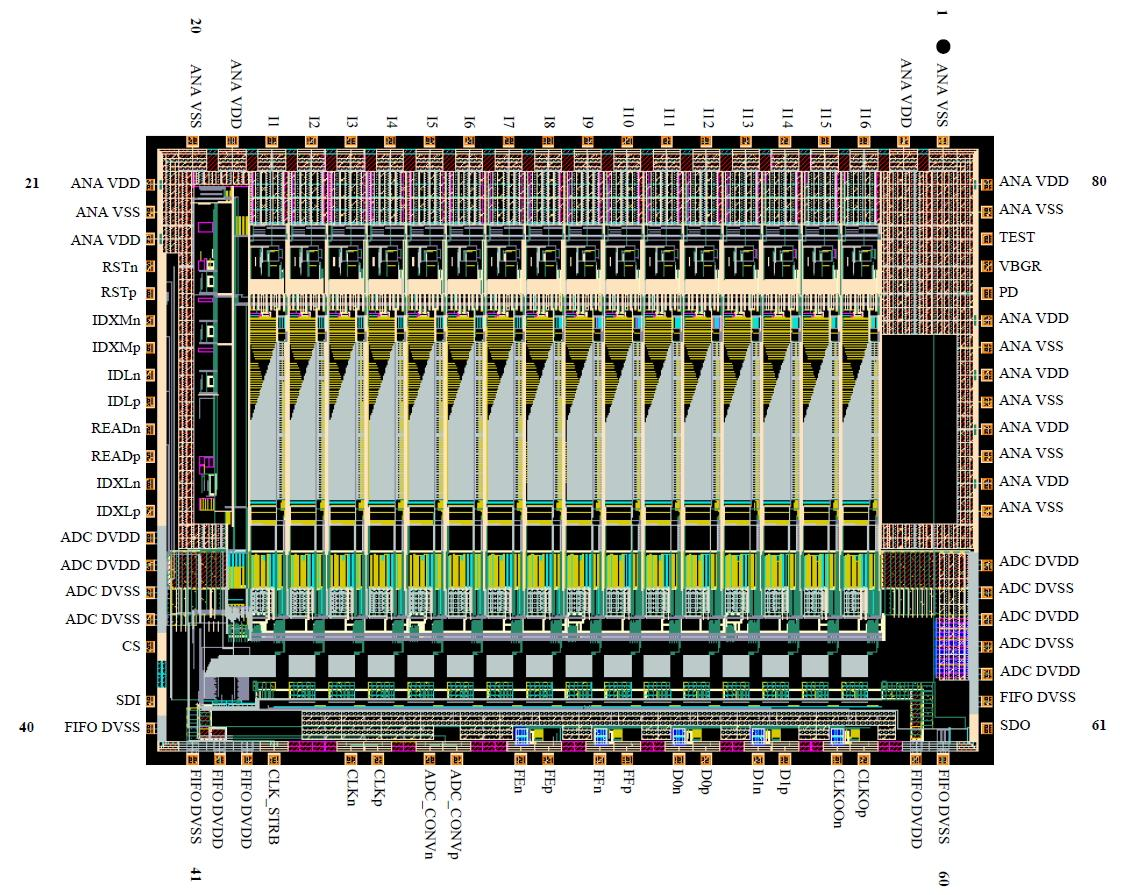
\includegraphics[width=\linewidth]{tpcce_ADC_ASIC_pinout.jpg} % New one
\end{cdrfigure}

The ADC ASIC has an input buffer with offset compensation to match the output of the FE ASIC.
The input buffer first samples the input signal (with a range of 0.2~V to 1.6~V),
then provides a current output after compensating for offset voltage error.
This current output is then supplied to the ADC which converts the input to digital in two phases.
The MSB (Most Significant Bit) 6~bits are first determined followed by the LSB (Least Significant Bit) 6~bits.
After the conversion the thermometer code is converted to binary and latched.
The output of ADC channel 16 can be monitored externally.
The data from the 16 ADCs are transferred in parallel to the FIFO block.
The built-in FIFO is 32~bits wide and 192~bits long,
and has full and empty indicator flags, needed for interfacing to the FPGA.
The ADC along with the input buffers are biased internally using a bias generator and a bandgap voltage reference.
The bandgap voltage (VBGR) can be monitored and/or controlled externally.
It can be put in the low-power sleep mode, and woken up in less than 1~$\mu$s.

Prototypes have been evaluated and characterized at RT (300~K) and LN2 (77~K) temperature.
During these tests the circuits have been temperature-cycled multiple times.
The effective resolution with reference to the input referred noise is $\sim$11.6~bits at both 300~K and 77~K.
The differential non-linearity (DNL) is less than 4 LSBs for 99\% of ADC bins at both 300~K and 77~K.

 
 
 The ADC outputs are passed to the FPGA mezzanine board for transmission to the warm electronics
 located on the outside of the signal flange.
The FPGA has four 4:1 MUX circuits that combine the 16 serial lines from the eight ADC
channels into four serial lines of 32 channels each, and 
four $\sim$1.2 Gigabit-per-second (Gbps) serial drivers that drive the data in each
line over cold cables to the WIBs.

\begin{cdrfigure}[The CE Architecture]{tpcce_schem}{The CE Architecture. The basic unit is the 128-channel FEMB.}
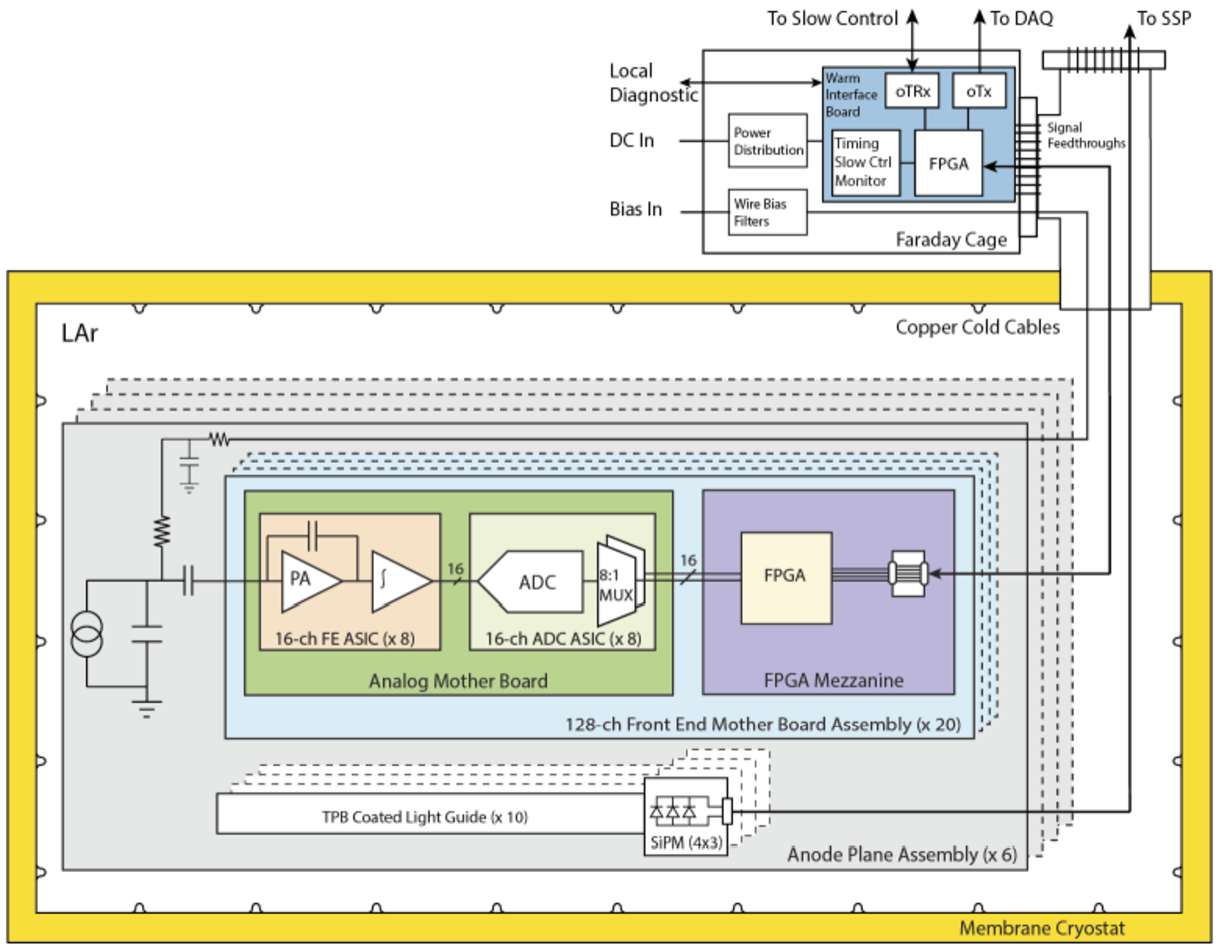
\includegraphics[width=0.9\linewidth]{tpcce_schem.pdf}
\end{cdrfigure}

\begin{cdrfigure}[The Front End Mother Board (FEMB), as used in an early set of tests]{tpcce_CMBpix}
{The Front End Mother Board (FEMB), as used in the early set of tests.
  {\bf Top:} The analog mother board, showing four ADC ASICs and four FE ASICs surface mounted.
  The other side of the board has another four ADC and FE ASICs.
  Except for anticipated small modifications, this board is essentially the final version.
  {\bf Middle:} The FPGA mezzanine, used in place of the digital ASIC mezzanine for the early set of tests.
  {\bf Bottom:} The complete FEMB assembly as used in the early set of tests.
  The cable shown in the high-speed data, clock, and control cable.}
\includegraphics[width=0.65\linewidth]{tpcce_CMBpix_1.pdf}
\includegraphics[width=0.65\linewidth]{tpcce_CMBpix_2.pdf}
\includegraphics[width=0.45\linewidth]{tpcce_CMBpix_3.pdf}
\end{cdrfigure}

The data are passed through the signal flange to the WIBs on copper cables utilizing LV differential signaling (LVDS).
On the WIBs, the data is further MUXed by 4:1 and transmitted over optical
fibers to the DAQ system described in Section~\ref{sec:DAQ_online_interface}.

The FPGA on the mezzanine card is also responsible for communicating with the
DAQ and timing systems and providing the clock and control signals required by the FE and ADC ASICs.

Each FEMB is enclosed in a Faraday box to provide shielding from noise. 
As shown in Figure~\ref{fig:tpcce_box}, the Faraday box is designed to make the electrical connection 
between the FEMB and the APA frame. %, as defined in Section~\ref{subsec:ele_design}. Not sure what section to reference.
 Mounting 
hardware inside the Faraday box connects the common plane of the FEMB to the box casing. The
box casing is electrically connected to the APA frame via twisted conducting wire (not 
shown in Figure~\ref{fig:tpcce_box}). This is the only point of contact between the FEMB and
APA, except for the input amplifier circuits connected to the CR board, which also terminate to
ground at the APA frame, as shown in Figure~\ref{fig:tpcce_cr_board}.

\begin{cdrfigure}[Faraday box for the FEMB]{tpcce_box}{Faraday box for the FEMB.}
\includegraphics[width=3in]{tpcce_box_1.pdf}
\includegraphics[width=3in]{tpcce_box_2.pdf}
\end{cdrfigure}

%
%%%%%%%%%%%%%%%%%%%%%%%%%%%%%%%%
\subsection{CE feedthroughs and cold cables}
\label{subsec:ce_feedthrough}

All cold cables originating from inside the cryostat connect to the outside warm electronics through PCB board feedthroughs
installed in the signal flanges that are distributed along the cryostat roof (Figure~\ref{fig:tpcce_FT_InternalCableRoute}).
The TPC data rate per APA, with an overall 32:1 MUX and 80 $\sim$1~Gbps data channels per APA,
is sufficiently low that the signals can be driven over copper LVDS tansmission lines.
Additional LVDS transmission lines are available for the distribution of clock signals and control information,
which are transmitted at a lower bit rate.
Optical fiber is employed externally from the WIBs on the signal flange to the DAQ and slow control systems.

\begin{cdrfigure}[Conceptual design of CE feedthrough]{tpcce_FT_InternalCableRoute}{
The CE feedthrough configuration and internal cable routing. The left panel shows a cutaway view of the cryostat.
The right panel shows more detail at the Faraday boxes.}
\includegraphics[width=7in]{tpcce_FT_InternalCableRoute.pdf}
\end{cdrfigure}


\begin{cdrfigure}[Conceptual design of CE feedthrough]{tpcce_signal_FT}{
TPC CE feedthrough. The WIBs are seen edge-on in the left panel,
and in an oblique side-view in the right panel, which also shows the warm crate for a DUNE module in a cutaway view (for 
ProtoDUNE-SP, there is a crate only on one side).}
\includegraphics[width=0.6\linewidth]{tpcce_signal_FT.pdf}
\end{cdrfigure}

The current design of the signal flange includes a T-shaped pipe, separate PCB feedthroughs for the CE and PDS cables, and
an attached crate for the TPC warm electronics, as shown in Figure~\ref{fig:tpcce_signal_FT}.
The wire-bias voltage cables connect to standard SHV connectors machined directly into the CE feedthrough,
ensuring no electrical connection between the wire-bias voltages and other signals passing through the signal flange.
Each CE feedthrough serves the bias/power/digital IO needs of one APA, as shown 
in Figure~\ref{fig:tpcce_cable_routing}.  

\begin{cdrfigure}[TPC cable routing scheme]{tpcce_cable_routing}{TPC cable routing scheme for three APA section.}
\includegraphics[width=0.9\linewidth]{tpcce_cable_routing.pdf}
\end{cdrfigure}

A program for minimizing potential contamination of the LAr from the cable plant contained within the ullage
(the warmer gas phase at the top of the cryostat) 
is being carefully followed.


Data/control cable bundles are used to send system clock and control signals from the 
signal flange to the FEMB, stream the $\sim$1~Gbps high-speed data from the FEMB to the signal flange, and 
provide backup JTAG programming to the cold FPGA, in case the power-up programming from the onboard 
EEPROM fails. As described in Section~\ref{subsec:ce_intro}, each FEMB 
connects to a signal flange via one data cable bundle, leading to 20 bundles between one APA and one flange.
Each data bundle contains 12 low-skew copper twin-axial cables with a drain wire, 
to transmit the following differential signals:

\begin{itemize}
    \item 4$\times$1.2~Gbps high-speed data
    \item One 50~MHz system clock
    \item One 2~MHz CONVERT clock
    \item 2 I2C control and configure
    \item 4 single-ended JTAG programming for the FPGA
\end{itemize}

The selected cables are Samtec 26~AWG twin-axial bundles with Samtec HSEC08 connectors to both
the FEMB mezzanine board and the signal flange. 
The HSEC08
connectors lock into place with tabs on each side of the connector. A sample of the Samtec cable with
THV outer jacket has passed outgassing tests in the LAr Materials Test Stand at Fermilab.

The Samtec 26~AWG cable has been
tested and demonstrated to have low enough dispersion such that both the LVDS 50~MHz system clock and
$\sim$1~Gbps high-speed data can be recovered over 25~meters of RT cable, 
significantly longer than the required seven meters needed to run cables between the FEMBs and signal flanges.

\begin{cdrfigure}[Results from cable validation testing]{tpcce_samtec_results}{Eye diagrams 
from cable validation testing. {\bf Top Left:} 50~MHz system clock over 25~m RT  
(RT) Samtec 26AWG cable. For comparison, {\bf Bottom Left} shows the same clock over 
the heavier, prohibitively expensive Gore 24AWG cable. {\bf Top Right:} 1~Gbps data over 
7~m (ProtoDUNE length) RT Samtec 26AWG cable without active recovery by equalizers. {\bf Bottom Right} 1~Gbps
data over 25~m (DUNE length) RT Samtec 26AWG cable with active recovery.}
\includegraphics[width=0.9\linewidth]{tpcce_samtec_results.pdf}
\end{cdrfigure}

Figure~\ref{fig:tpcce_samtec_results} shows results from the cable 
validation testing. The eye diagrams show the edges of the differential signals after 
LVDS transmission over the specified cable types and lengths. The height of eye diagram shows the size 
of the recovered signal in mV and the slope of the rising and falling edges are jitter in picoseconds (ps). 
An eye diagram is sufficient to show that the edges of the differential signals can
be recovered, but not enough to demonstrate the bit error rate (BER). However, the Samtec 26~AWG cable has 
also passed a BER test, transmitting $10^{13}$ bits without error.



LV power is passed from the signal flange to the FEMB by bundles of 16 Samtec 
20~AWG twisted-pair wires, as shown in Figure~\ref{fig:tpcce_cable_routing}. One IPD1 connector
attaches all 16 wires at the signal flange, and two IPD1 connectors are attached to the FEMB (one to the
analog motherboard and one to the FPGA mezzanine). In total, 20 wire bundles 
 bring LV power to the FEMBs associated with one APA.

Eight of the 16 wires are power feeds, as described in Figure~\ref{fig:tpcce_lv_req}. The other eight wires
are attached to the common of the input amplifier circuits, as described in Section~\ref{subsec:ce_wire_bias}.
For
a single FEMB, the resistance is $<30$~m$\Omega$ at RT or $<10$~m$\Omega$ at LAr temperature. Each APA has a copper cross-section of approximately $80~\mathrm{mm}^2$, with
a resistance $<1.5$~m$\Omega$ at RT or $<0.5$~m$\Omega$ at LAr temperature.

\begin{cdrfigure}[LV power feed wire specifications]{tpcce_lv_req}{Samtec LV power feed wire 
specifications.}
\includegraphics[width=4in]{tpcce_lv_req.pdf}
\end{cdrfigure}

%\fixme{Eric questions whether figure~\ref{fig:tpcce_lv_req} is needed}

The wire-bias voltage cables are required to deliver voltages up to a few thousand Volts and currents up to a few
milliAmps.

The bias voltages are applied to the X-, V-, and G-plane wire layers, three field cage terminations, 
and an electron diverter, as shown in Figure~\ref{fig:tpcce_cr_board}. The voltages are supplied 
through eight SHV connectors mounted on the signal flange. RG-316 coaxial cables carry the voltages 
from the signal flange to a patch panel PCB which includes noise filtering mounted on the top 
end of the APA. 

From there, wire-bias voltages are carried by single wires to 
various points on the APA frame, including the CR boards, a small PCB mounted on or near 
the patch panel that houses a noise filter and termination circuits for the field cage voltages, and 
a small mounted board near the electron diverter that also houses wire-bias voltage filters.


%%%%%%%%%%%%%%%%%%%%%%%%%%%%%%%%    
\subsection{Warm interface electronics}
\label{subsec:warm_interface_elec}

The warm interface electronics are housed in warm electronics crates (WECs)
attached directly to the signal flange.  The WEC shown in Figure~\ref{fig:tpcce_ceflange_sbnd} 
contains one
Power and Timing Card (PTC), up to five Warm Interface Boards (WIBs) and a passive
backplane (PTB), which fans out signals and LV power from the PTC to the WIBs.

\begin{cdrfigure}[Conceptual design of signal flange]{tpcce_ceflange_sbnd}{Exploded view of 
the signal flange for SBND (ProtoDUNE-SP has five WIBs).}
\includegraphics[width=0.9\linewidth]{tpcce_ceflange_sbnd.png}
\end{cdrfigure}

The WIB is the interface between the
DAQ system and up to four
FEMBs. It receives the system clock and control signals from the
timing system and provides for processing and fan-out of those signals to the four
FEMBs. The WIB also receives the high-speed data signals from the four 
FEMBs and transmits them to the DAQ system over optical
fibers.  The WIBs are attached directly to the TPC
CE feedthrough on the signal flange. The feedthrough
board is a PCB with connectors to the cold signal and LV power cables fitted
between the compression plate on the cold side, and sockets for
the WIB on the warm side. Cable strain relief for the cold cables is 
supported from the back end of the feedthrough.


%%%%%%%%%%%%%%%%  
%\subsubsection{Power and Timing Card}
%\label{subsubsec:power_timing_card}

\begin{cdrfigure}[PTC and timing]{tpcce_wib_timing}{Power and Timing Card (PTC) 
and timing distribution to the WIB and FEMBs.}
\includegraphics[width=0.5\linewidth]{tpcce_wib_timing.jpg}
\end{cdrfigure}

The PTC provides a bidirectional fiber interface to the
timing system.  The received data is separated into clock and
data using a clock/data separator.  The clock and data
streams are separately fanned-out to the five WIBs as shown in
Figure~\ref{fig:tpcce_wib_timing}. The PTC fans the clocks out to the WIB over the
PTB, which is a passive backplane attached directly to the PTC and
WIBs.

\begin{cdrfigure}[WIB and LV power]{tpcce_wib_power}{LV power distribution 
to the WIB and FEMBs. 200~W is for a fully-loaded crate 
with the majority of the power dissipated by the 20 cold FEMBs in the LAr.}
\includegraphics[width=0.6\linewidth]{tpcce_wib_power.pdf}
\end{cdrfigure}

The PTC also receives LV power for all cold
electronics connected through the signal flange, approximately 200~W at 12~V for a
fully-loaded flange (five~WIB + 20~FEMB). The LV power is then fanned out
on the PTB to each WIB, which provides the necessary DC/DC conversions and fans
the LV power out to each of the cold FEMBs supplied by that WIB, 
as shown in Figure~\ref{fig:tpcce_wib_power}. The 
majority of the 200W drawn by a full flange is dissipated in the LAr
by the cold FEMB.


%%%%%%%%%%%%%%%%  
%\subsubsection{Warm Interface Board}
%\label{subsubsec:warm_interface_board}

Each WIB contains a 
unique IP address for its UDP slow control interface. The IP address for the WIB is 
derived from a crate and slot address: the crate address is generated on the PTC 
board via dipswitches and the slot address is generated by the PTB slot, numbered 
from one to five. Note that the WIBs also have front-panel
connectors for receiving LV power; these can be used in place of 
the LV power inputs on the PTB generated by the PTC.

The WIB is also capable of
receiving the encoded system timing signals over bi-directional optical
fibers on the front panel, and processing these using either
the on-board FPGA or clock synthesizer chip to provide the 50~MHz
clock required by the cold electronics.  

\begin{cdrfigure}[Warm Interface Board]{tpcce_dune_wib}{Warm interface board (WIB). Note 
that front panel inputs include a LEMO connector and alternate inputs for LV power.}
\includegraphics[width=0.9\linewidth]{tpcce_dune_wib.jpg}
\end{cdrfigure}

The FPGA on the WIB is an Altera Arria V GT variant, which requires a
125~MHz clock for its state machine that is provided by an on-board crystal
oscillator. The GT variant of the Arria V
transceivers can drive the high-speed data to the DAQ system up to
10.3125~Gbps per link,  implying that all data from
two FEMB (2$\times$5~Gbps) could be transmitted on a single link. However, it is planned to
use a QSPF socket on the WIB to deliver $\sim$5~Gbps on four optical fibers 
(one fiber per FEMB) to two RCEs. \fixme{write out} The FPGA has an additional Gbps Ethernet
transceiver I/O based on the 125~MHz clock, which provides real-time digital data readout to the slow control system.



%
%%%%%%%%%%%%%%%%%%%%%%%%%%%%%%%%  
\subsection{External Power and Cables}
\label{subsec:ce_feedthrough_power}

The LV power to the FEMB and WIB is supplied by Weiner MPOD power supplies. 
\fixme{define MPOD}
The CE power-per-channel is about 25~mW in the LAr.
Including power for the WIB, a fully loaded WIB (one WIB plus four FEMBs) requires
12V and draws approximately 3.3~Amps. Therefore, the full electronics for one APA (five WIBs + 20 FEMBs) 
requires 12~V and draws approximately 16~Amps, for a total power of almost 200~W, as 
described in Section~\ref{subsec:warm_interface_elec}.

Each MPOD LV power unit has two DSUB37 connectors, each with four channels of LV output, including negative
and positive sense wires. %as shown in Figure~\ref{fig:tpcce_mpod_top}. 
Each channel has three pins
of negative output and three pins of positive output. Five of the eight channels
provide the 12~V/3.3~A to each WIB via the PTC, and one channel provides LV power 
to the PTC itself, with two of the eight channels unused.

%\begin{cdrfigure}[MPOD DSUB37 top connector]{tpcce_mpod_top}{MPOD DSUB37 top connector.}
%\includegraphics[width=1.0\linewidth]{tpcce_mpod_top.png}
%\end{cdrfigure}

Each MPOD wire-bias voltage unit supplies the wire-bias voltages to eight SHV connectors 
at the signal flange. One MPOD chassis contains three LV and three wire-bias units, and can
supply all the LV and wire-bias power to three APAs worth of cold electronics. Therefore,
a total of two MPOD chassis are required for the detector.


The LV power cable uses DSUB37 connectors. The bottom of the fuse PCB at the MPOD 
end of the cable is shown in Figure~\ref{fig:tpcce_fused_cable}. Each of the three output pins on
each channel are tied together in parallel 
going to one wire large enough to carry the full supply voltage. Fuses can optionally be 
populated on each output pin as shown in Figure~\ref{fig:tpcce_fused_cable}; however, if
fusing is not selected, the pins will be connected with 0~$\Omega$ resistors. This fusing would serve as
a final protection. The primary protection would come from the Over Current protection
on the MPOD, which is set above the 3.3~A required by each WIB, but below the
combined fuse value.

\begin{cdrfigure}[Bottom of the fuse PCB]{tpcce_fused_cable}{Bottom of the fuse PCB at the MPOD end of the cable.}
\includegraphics[width=0.7\linewidth]{tpcce_fused_cable.png}
\end{cdrfigure}

The five separate 12~V/3.3~A channels to the WIBs are delivered to the PTC using two normal DSUB37 connectors to
attach the LV power cable. The fusing for the sense wires is implemented on the PTC.

Each APA requires three wire-bias voltage connections 
at $+$820V, $-$370V, and $-$665V, as described in Section~\ref{subsec:ce_wire_bias}.
The current on each of these supplies is expected to be zero at normal operation.
However the ripple voltage on the supply must be carefully controlled 
to avoid noise injection into the front-end electronics.

RG-58 coaxial cables connect the wire bias voltages from the MPOD to the standard SHV
connectors machined directly into the CE feedthrough, so there is no electrical connection between 
the LV power and data connectors and wire-bias voltages. The length of the cables from the Weiner MPODs
to the signal flanges is estimated to be 18~meters.


Optical fibers provide the connections between the WECs, which act as
Faraday-shielded boxes, to the DAQ and slow control systems.
Each WIB uses QSFP sockets for 
four pairs of fiber, %as described in Section~\ref{subsubsec:warm_interface_board}, 
implying a total of 120 optical data fibers for the 30 WIB boards in the system. The optical fibers from
the signal flanges to the DAQ room are estimated to be 30$-$40~m in length.

Duplex LC optical fiber is under consideration for transmitting the one GIG-E connection from each
WIB to the slow control system. The WIB reports the current draw from each FEMB to the slow control system, while the 
current draw for each WIB is monitored at the MPOD itself.



%%%%%%%%%%%%%%%%%%%%%%%%%%%%%%%%%%%%%%%%%%%%%%
\section{Photon Detection System (PDS)}
\label{sec:pd_system}

LAr is an excellent scintillating medium and the photon detection
system will exploit this property in the far detector.  With an
average energy of 19.5~eV needed to produce a photon (at zero field),
a typical particle depositing 1~MeV in LAr will generate
40,000~photons with wavelength of 128~nm. At higher fields this will
be reduced, but at 500~V/cm the yield is still $\sim$20,000~photons
per MeV. Roughly 1/4 of the photons are promptly emitted with a
lifetime of about 6~ns while the rest have a lifetime of
1100--1600~ns. Prompt and delayed photons are detected in
  precisely the same way by the photon detection system. LAr is
highly transparent to the 128-nm VUV photons with a Rayleigh
scattering length of (66~$\pm$~3)~cm~\cite{Rayleigh} and absorption
length of $>$200~cm; this attenuation length requires a LN$_2$
  content of less than 20~ppm. The relatively large light output makes
the scintillation process an excellent candidate for determination of
$t_0$ for non-beam related events. Detection of the scintillation
light may also be helpful in background rejection and triggering on
non-beam events.

%%%%%%%%%%%%%%%%%%%%%%%%
\subsection{Scope and requirements}

The scope of the photon detector system (PDS) for the ProtoDUNE-SP detector
includes design, procurement, fabrication,
testing, delivery and installation of the following components:
\begin{itemize}
\item Light collection system including wavelength shifter and light guides
\item Light sensors: Silicon photo-multipliers (SiPMs)
\item Readout electronics
\item Monitoring system
\item Related infrastructure (frames, mounting boards, etc.).
\end{itemize}

The photon detection system reference design described in this section
will determine if the detector meets the required performance for 
light collection for the DUNE far detector. 
The primary requirement is the detection of light from proton decay
candidates (as well as beam neutrino events) with high efficiency to
enable 3D spatial localization of candidate events. The light yield that
has been required for this is 0.1\,pe/MeV at the cathode plane.
The TPC will provide supernova neutrino detection, while the detection of light
from supernova neutrino interactions should localize the events and disentangle
them from background noise in the TPC detection.
The photon system will provide the $t_0$ timing of
events relative to TPC timing with a resolution better than 1~$\mu$s
(providing position resolution along the drift direction of a couple of mm). 
Measurements from the ProtoDUNE-SP detector will determine the absolute
light yield by measuring light from beam particles and cosmic ray muons
tracked in the TPC or identified by external muon trigger counters.
Informed by this light yield measurement the determination of whether the 
light yield is sufficient for the required science goals can be made.

Figure~\ref{fig:PD_overview} shows the layout for the photon detector
system described in this section. %, which will be described in the following sections.

\begin{cdrfigure}[Photon detection system overview]{PD_overview}{Overview of the PDS
    system showing a cartoon schematic (a) of a single PDS module
    in the LAr and the channel ganging scheme used to reduce the
    number of readout channels. Panel (b) shows how each PDS module
    will be inserted into an APA frame. There will be 10 photon detectors (PDs) inserted
    into an APA frame.}
\includegraphics[width=1.0\linewidth]{pd_schem.png}
\end{cdrfigure}

%%%%%%%%%%%%%%%%%%%%%%%%%%
\subsection{Photon detector modules}

Two styles of PDS %photon detector (PD) 
modules are being produced for ProtoDUNE-SP.  
The concepts are very similar, but differ in the number of times the LAr scintillation 
light is shifted.  

The reference design shown schematically in Figure~\ref{fig:PD_overview}
has wavelength-shifting radiator plates mounted on a wavelength-shifting light guide.
The plates are coated 
with tetraphenyl-butadiene (TPB) to produce blue ($430nm$) light from the $128nm$ VUV 
scintillation light.  
This blue light is absorbed by a commercially produced wavelength shifting (WLS)
polystyrene bar with Y-11 fluor.  
The bar serves as a light guide to transmit the green light to the photosensor 
mounted at its end.
The radiator plates are captive in mounting blocks that are glued to the WLS bar
at regular intervals as shown in Figure~\ref{fig:PD_radiator_mount}.

\begin{cdrfigure}[Radiator Plate Mounting Blocks]{PD_radiator_mount}
  {Mounting of the radiator plates to the WLS bar for the reference design scheme}
\includegraphics[width=0.5\linewidth]{PD_radiator_mount.PNG}
\end{cdrfigure}

The alternative design uses the same photodetector and mounting, but does not have
any radiator plates mounted on it.  
Instead, the bar is made by dip-coating an acrylic light guide with a solution
of TPB, solvents, and a surfactant to produce a bar with the wavelength shifter coated
on the outside.  
It has only one wavelength shifting step, which should increase the efficiency.  
Previous work for DUNE with this technique showed that the attenuation length, and
therefore the light yield, would suffer from the coating process, but bars produced with
the latest technique as shown in~\cite{conrad_jinst2015} have %been shown to have 
avoided this problem.




%%%%%%%%%%%%%%%%%%%%%%%%%%
\subsection{Sensors}
The planned photodetector is a SiPM.  
The model planned for ProtoDUNE-SP is the SensL C-Series 6~mm$^2$
(MicroFB-60035-SMT) device. These SiPMs have detection efficiency of
41\%; the detection efficiency combines QE and effective area
  coverage accounting for dead space between pixels.   At LAr temperature (89~K) the dark rate is of order 10~Hz
(0.5 p.e. threshold) while after-pulsing has not been an
issue. Extensive testing is underway and will continue, to ensure 
that the SiPMs can reliably survive the stresses associated with 
any thermal cycling in LAr and long-term operation at LAr temperature.

All photodetectors for ProtoDUNE-SP will be subjected to testing to determine
 forward and reverse bias I-V curves,
 breakdown voltage, dark current and dark count rate, photodetector gain, crosstalk estimation, response, and bias dependence of parameters.
 
%All SiPMs 
Each SiPM will be tested before mounting on the readout boards to determine
if the part meets the specifications in a warm test.  After mounting to
the readout board all items will be tested both warm and cold (cyrogenic 
temperature) to determine the operating characteristics as when %they will be 
installed at the ProtoDUNE-SP detector, and during QA/QC tests on the PDS modules.

In addition to these tests, the photodetectors will be tested for their
response to light signals from an LED with appropriate wavelength.
These tests will be sensitive enough to determine if one of the three SiPM
elements in parallel is not functioning.


%%%%%%%%%%%%%%%%%%%%%%%%%%
\subsection{Mechanical design and installation}
  % -- CSU  -- Dave
  %  Mechanical Design Mounting 

The PDS system is configured as a set of \textit{modules} that are mounted on the APA frames.  A PDS module is
the combination of one light guide (also called a ``bar'' due to its
shape) and 12 SiPMs, as shown in Figure~\ref{fig:PD_overview}~(a). 
 %To enable this, the the reference design for mounting the PDs onto the
The reference design for the APA frames calls for ten PDS modules per APA, approximately 2.2-m long,
86-mm wide and 6-mm thick, equally spaced along the full length of the
APA frame, as shown in Figure~\ref{fig:PD_overview}~(b). 
The light guides are inserted into the APA frame on rails gliding on their radiator
plate mounting blocks, as shown in Figure~\ref{fig:PD_mounting_inslide} (right). \fixme{check if right figure ref}

\begin{cdrfigure}[Diagram of PDS installation into APA frame and installed SiPM mounting board]
  {PD_mounting_inslide}{(left) Rendering of the installation of a PDS module
    into an APA frame, shown just before it comes to rest on the inside face
    of the APA tube. (right) Rendering of the the SiPM mounting board
    installed on the end of the PDS module before insertion.}
\includegraphics[width=0.45\linewidth]{PD_mounting_inslide.PNG}
\includegraphics[width=0.45\linewidth]{PD_endblock_mnt.PNG}
\end{cdrfigure}
%
%\begin{cdrfigure}[SiPM mounting board attached to PDS module]
 % {PD_endblock_mnt.PNG}{Rendering of the the SiPM mounting board
  %  installed on the end of the PDS module before insertion.}
%\includegraphics[width=0.50\linewidth]{PD_endblock_mnt.PNG}
%\end{cdrfigure}


The system has been prototyped and test fitted with a module at CSU 
as shown in Figure~\ref{fig:PD_flat_installtest}.
\begin{cdrfigure}[Photo of PD mock installation]
  {PD_flat_installtest}{Photograph of the installation
    test of a mock PDS module in a 1/5 section of an APA frame.}
\includegraphics[width=0.50\linewidth]{pd_flat_installtest.jpg}
\end{cdrfigure}

  %   Mechanical Design SiPM mounting board

Each photon detector has a single SiPM mounting board with 12 surface-mount SiPMs 
mounted on the face as in Figure~\ref{fig:PD_SiPM_PCB_front} (left).
Four groups of $3$ SiPM elements will go to a single 
channel of readout electronics in order to reduce the cost of the readout.
The board is held close to the bar, without touching, by four screws that go into 
tapped holes on the end mounting block that is glued to the bar.  
The mounting block assembly is shown in Figure~\ref{fig:PD_mounting_inslide} (right) %\ref{fig:PD_endblock_mnt}.
The circuit board also has holes at each end for mounting to the APA frame.  

\begin{cdrfigure}[SiPM mounting board with 12 SiPMs and with Rj-45 connector]
  {PD_SiPM_PCB_front}{Photograph of a SiPM mounting board
    with the full complement of 12 SiPMs installed on the board (left), and with the 
    RJ-45 connector for the cable (right).}
\includegraphics[width=0.55\linewidth]{PD_SiPMMountPCB_front.PNG}
\includegraphics[width=0.4\linewidth]{PD_SiPMMountPCB_back.PNG}
\end{cdrfigure}
%\begin{cdrfigure}[Readout board with RJ-45 connector]
%  {PD_SiPMMountPCB_back}{Photograph of the SiPM readout PCB with the 
%    RJ-45 connector for the cable.}
%\includegraphics[width=0.50\linewidth]{PD_SiPMMountPCB_back.PNG}
%\end{cdrfigure}

  %   Mechanical Design Cabling

The cabling plan for the system has one cable with four shielded twisted pairs 
connected to each SiPM mounting board via the surface mount RJ-45 connector
shown mounted on the back of the readout PCB in 
Figure~\ref{fig:PD_SiPM_PCB_front} (right).  
The cables run through the APA tubing to the top of the APA frame as seen
in Figure~\ref{fig:PD_cable_intube}.
The cable bundles are installed and connected to each PD 
after the PD has been installed into the slot.
\begin{cdrfigure}[Cables in APA frame]
  {PD_cable_intube}{Diagram showing the routing of the PDS cables
    through the APA frame.}
\includegraphics[width=0.50\linewidth]{PD_cable_intube.PNG}
\end{cdrfigure}


%%%%%%%%%%%%%%%%%%%%%%%%%%
\subsection{Alternative photo detector under development}

%\fixme{add citation to bib:
% arapuca_jinst 
%A.A. Machado and E. Segreto, \emph{ARAPUCA a new device for liquid argon scintillation light detection}, {JINST}  {\bf 11} (2016) C02004.
%}
%\section{The ARAPUCA device}
While a sufficient number of the two standard arrays are being produced to fully outfit protoDUNE-SP, it is possible that some will bays will have experimental detectors installed in place 
of the 4 standard arrays. One type of detector that is being developed in an attempt to increase the light detection eficiency is called an ARAPUCA.

The ARAPUCA is a device based on a new technology that should allow to collect photons with a window of big area with detection efficiencies at the level of several percent while using 
active photon detectors with much smaller area.
The fundamental idea at the basis of the ARAPUCA is to trap photons inside a box with highly reflective internal surfaces, so that the detection efficiency of trapped photons is high even with a  limited active coverage of its internal surface \cite{arapuca_jinst}.

Photons trapping is achieved by using a clever wavelength-shifting technique coupled with the technology of the dichroic shortpass optical filters. The latter are multilayer acrylic films 
with the  property of being highly transparent to photons with a wavelength below a tunable cut-off while being almost perfectly reflective to photons with wavelength above the cut-off. 
A dichroic shortpass filter deposited with two different wavelength shifters (one on each side) will be the core of the device. In particular, it will be the acceptance window of the 
ARAPUCA. The rest of the device will be a flattened box with highly reflective internal surfaces (PTFE, 3M-VIKUITI ESR, \dots), closed on the top by the 
dichroic  filter deposited with the two shifters. A fraction of the box internal surface is occupied by the active photo-sensors (Silicon Photomultipliers - SiPM) which will detect the trapped photons.

Two arrays of small ARAPUCAs will be installed inside protoDUNE to test the devices in a real experimental situation and to directly compare their performances with those of the guiding 
bars and other eventual alternative photon detection schemes.\
The arrays will be compatible with the mechanical solutions foreseen for the guiding bars and will have zero impact on the construction of the detector. In particular each one of the two 
arrays will replace one bar. It will be composed by 8 ARAPUCAs/bar (for a total of 16 devices)  as shown in figure \ref{fig:arapuca_array}.
%*****************************FIGURE 2*****************************%
\begin{figure}[t]
\begin{center}
\includegraphics*[width=8.cm]{APA_ARAPUCA}
\caption{ {\it One ARAPUCA array of 8 devices installed in a APA frame in place of a scintillating bar.}}
\label{fig:arapuca_array}
\end{center}
\end{figure}
%***********************************************************************%
Each ARAPUCA will be a teflon box with dimensions of 5$\times$5$\times$1 cm$^3$ with an acceptance window of 5$\times$5 
cm$^2$ and the trapped light will be detected by 2 SIPM (SensL 60035 - 6$\times$6 mm$^2$ active area each). The readout scheme foresees the ganging of the SiPMs from two ARAPUCAs (4 sensors) so that each array will require 4 channels, which will use the same cabling and the same SSP read-out of the guiding bars.

%%%%%%%%%%%%%%%%%%%%%%%%%%
\subsection{Photon detector UV-light monitoring system}
\label{sec_pd_calib}

\fixme{Need to reduce to 1-2 pages, (flavio)}
%Items relevant to the PDS calibration are the fast and slow components of the light, photon propagation including scattering and reflections, impact of N$_2$, E-field strength, 
%and the energy range of interest. A calibration system that addresses these issues has to be both comprehensive and cost-effective, and has to be tied to the overall 
%calibration system for ProtoDUNE-SP, which includes both charge and scintillation light calibration techniques. 
%In addition, there is a need to evaluate relative efficiencies of multiple PD units and monitor response and stability of the system as a function of time.

A UV-light-based monitoring system that will serve to monitor the relative performance and time resolution of the system has been designed. % and is described here.
The system will consist of a set of UV LEDs as light sources in the VUV wavelength range, coupled to quartz fibers, to transmit light from outside the detector volume to desired locations at the CPA within the TPC.
Light diffusers located at the CPA surface will uniformly illuminate the APA area with photon-detector system (PDS) elements.
The light sources located and fired externally, with fibers running into the cryostat to diffusers that will emit light from the CPA to the APA. 
For the ProtoDUNE-SP cryostat at the surface at CERN, the UV light system will be complementary to cosmic ray muon 
tracks and Michel electrons as means of calibration. In terms of light sources the measurements will be performed with an UV (245-280) light source.
The UV light essentially mimics physics, although at a different wavelength starting from the wavelength-shifter conversion, 
light guide propagation, photo-sensor detection and the front-end electronics readout.
	
The external UV-light monitoring system is designed with the following goals:
				
\begin{itemize}
\item Simple to implement (no active components within PD/APA, such as LEDs or fibers mounted within APA).
\item Uniformly illuminates APA surface with the light diffused from CPA locations.
\item Has a potential to be adapted for deployment in a large Far Detector in the future
\end{itemize}

In terms of technical requirements the system needs to:
\begin{itemize}
\item provide light levels down to a single p.e. at individual photon-detector channels,
\item provide higher light levels to test linearity of the PDS,
\item provide variable pulse width to test the time resolution of the photon detector response, and
\item uniformly illuminate the APA area of the detector for relative monitoring of the PDS channels
\end{itemize}

Figure~\ref{fig:fig-c-1} illustrates the system design schematically. The system consists of a 1U rack mount Light Calibration Module (LCM) sitting outside the cryostat. The LCM generates light pulses that propagate through a quartz fiber-optic cable to diffusers at the CPA to distribute the light uniformly across the photon detectors mounted within the APA.  ProtoDUNE-SP will have five light 
diffusers on the CPA plane: one in the center and four diffusers close to the CPA corners. 
%
 \begin{cdrfigure}[UV-light monitoring system]{fig-c-1}{Concept of the UV-light monitoring system for the photon detector in liquid argon.}
\includegraphics[angle=0,width=0.7\textwidth]{calPD_concept-from-35ton.pdf}
\end{cdrfigure}
%


The LCM utilizes the logic and timing control of the photon-detector readout electronics ("SSP") unit.  
An SSP board was repackaged into a deeper rack mount chassis that accommodates a new internal 
LED Pulser Module (LPM) and an additional bulk power supply. The LPM utilizes five digital outputs from the SSP board to control the LPM pulse and its duration.  
These outputs are derived from the charge injection control logic within the SSP's FPGA.  
The even-channel SiPM bias Digital to Analog Converters (DACs)
are used to control the LPM pulse amplitude.  
The adjacent odd channels are used to read out a reference photodiode used for pulse-by-pulse monitoring of the LED light output.  
The output of the monitoring diode may be used to normalize 
the response of the SiPMs in the detector to the monitoring pulse.


\fixme{A bunch of content removed from here; but then gap in (paper) pages received from Flavio (missing 4-147 to 4-180); not sure what to do with remainder of this file. Anne}

\fixme{How long do these monitoring run take ? When would they be taken (relative to beam and comics running) ? Some interference with light from comics is expected; how will this be addressed ? Time of a flash will be known much better then 1us, so not much overlap with random cosmic events at ~1ms }

The controlled source of light %described here 
in this monitoring system will be used to perform time offset and time resolution measurements.  
Many effects contribute to a finite time resolution, relative time offset of photon-detector channels, scintillation time constants, 
photon conversion with wavelength shifter, photon propagation through photon-detector paddle, SiPM jitter, and FEE resolution. 
Most of these effects are constant and can be individually 
measured on the bench.  The UV light monitoring system will monitor overall stability of the photon detector in both time
and amplitude.

%%%%%%%%%%%%%%%%%%%%%%%%%%%%%%%%%%%%%%%%%%%%%%
\section{PDS electronics}\label{sec:pds-elec-daq}

\fixme{this section needs some language editing}

Scintillation light from LAr comes from the two different excited 
states with lifetimes of about 6 ns and 1.6 $\mu$s. 
Only a limited amount of light is collected by this system, so we 
assume the electronics must be designed to collect the light 
from both excited states. A summary of the general requirements 
for the system, including initial requirements from a 
physics performance perspective, are given in Table~\ref{tab:fee_req}.
%

\begin{cdrtable}[Physics requirements for the PDS electronics]{ll}{fee_req}{Physics requirements for the PDS electronics}
 Performance Parameter       & Target   \\ \toprowrule
Time Resolution                   & Better than 30 ns wrt event time zero ("t0")      \\ \colhline
 Charge Resolution               & 0.25\% photo-electron equivalent                    \\ \colhline
 Dynamic Range                   & $\sim$ x10 better than detector (1000:1)         \\ \colhline
 Linearity                               & Sufficient to resolve 1 photo-electron signals   \\ \colhline
 Multi-Hit Capability              & Sufficient to measure Triplet (late) Photons          \\ \colhline
 Dead Time                           & Live up to 2 drift times either side of beam spill         \\ \colhline
 Bias Control                        & 0.1 V resolution up to 30 V per channel  \\ \colhline
 Calibration                          & On-board Charge Injection  \\ \colhline
 Timing                                 & Events time-stamped using NO$\nu$A Timing or equivalent syst.  \\    \end{cdrtable}

%
The plans for the electronics for the photon detection subsystem 
include a baseline design with several options 
that remain R\&D activities.   

In the baseline plan, there are no front-end electronics in the cold volume.  
The un-amplified signals from the SiPMs 
are transmitted to outside the cryostat %on cables 
for processing and digitization, with
the advantage that the infrastructure required for inside the cryostat is 
reduced (power, data cables, precision clocks, data protocols, etc.).  
%
A custom module, called the SiPM Signal Processor (SSP), receives the SiPM signals. % has been designed and built 
%for preprocessing for trigger and data acquisition (DAQ) in the front-end.
%to perform signal processing in the front-end as preprocessing for trigger and data acquisition (DAQ). 
%The module is called the SiPM Signal Processor (SSP).  

An SSP consists of 12 readout channels packaged in a self-contained 
1U module.  
Each channel contains a fully-differential voltage amplifier and a 
14-bit, 150 MSPS analog-to-digital converter (ADC) that 
digitizes the waveforms received from the SiPMs.  
The front-end amplifier is configured as fully-differential with high common-mode 
rejection, and receives the SiPM signals into a termination resistor that 
matches the characteristic impedance of the signal cable. 
Currently there is no shaping of the signal, since the SiPM response 
is slow enough relative to the speed of the digitization to obtain 
several digitized samples of the leading edge of the pulse for the determination of signal timing.  

The digitized data is stored in pipelines in the SSP, for up to $\sim$ 13 $\mu$s.  
The processing is pipelined, and performed by a Xilinx Artix-7 
Field-Programmable Gate Array (FPGA).  
The FPGA implements an independent Data Processor (DP) for each channel.  
The processing incorporates a leading edge discriminator for detecting events
and a constant fraction discriminator (CFD) for sub 
clock timing resolution.  
Because the FPGA is programmable and accessible, it is possible to explore 
different data processing algorithms and techniques, and even customize the 
readout for a given type of event (supernova for example.)  
A picture of the module is shown in Fig.~\ref{fig:PD_fig-e-2}.  
A block diagram of the system is shown in Fig.~\ref{fig:PD_fig-e-3}.
%Fig. xx3.  Picture of the SSP module.
%
\begin{cdrfigure}[SSP Photograph]{PD_fig-e-2}{Picture of SSP module.}
  \includegraphics[angle=90,width=0.5\textwidth]{PD_fig-e-2.png}
\end{cdrfigure}

\begin{cdrfigure}[SSP Block Diagram]{PD_fig-e-3}{Block diagram of the SSP Module.}
  \includegraphics[width=0.8\textwidth]{PD_fig-e-3.png}
\end{cdrfigure}
%
In the simplest mode of operation, the module can perform waveform capture, 
using either an internal trigger or an external trigger.  
Up to 2046 waveform samples may be read out for each event.  When waveform 
readouts overlap the device can be configured to offset, 
truncate or completely suppress the overlapping waveform.  
Pile-up events can also be suppressed.  

Generally, the SSP performs pipelined processing.  
The module has been designed to support several different triggering schemes, 
including self-triggered, use of an external trigger, or use an 
external gate to readout all events within a time-window.  
In order for the events measured in the photon detector to be matched up 
with the corresponding events in the TPC, the front-end electronics 
attaches a timestamp to the data as it is acquired.  
The timestamp is unique, and has a correspondence with the timestamps in 
the TPC electronics processing.  
The timestamp in the SSP is applied to the event data as it is digitized, 
and becomes part of the data as the processing proceeds.  
In the case where zero-suppression and data sparsification are used, 
the timestamp on accepted data remains intact.  
To achieve this, the TPC and PD electronics must be synchronized, 
including timestamp counter resets, and a known and stable calibration between 
the corresponding timing resolution of the ADC conversion in the two systems.  

A Xilinx Zynq FPGA, onboard the MicroZed system-on-module, handles the 
slow control and event data transfer.  
The SSP has two parallel communication interfaces; USB 2.0 and 10/100/1000 Ethernet.  
The 1 Gb/s Ethernet supports full TCP/IP protocol.  
The module includes a separate 12-bit high-voltage DAC for each channel to 
provide up to 30 V of bias to each SiPM.  
The module also feature charge injection for performing diagnostics and linearity 
monitoring, and also voltage monitoring.

In tests to date, the SSP is capable of measuring single photo-electron signals 
coming from the SiPMs over a cable length of 30 meters when the SiPMs are 
operated at LAr temperatures.  
The timing resolution of the signals has been measured to be better than 3 ns.  
The full-differential signal processing in the front-end circuitry 
is important in achieving this result.

The baseline plan assumes that three SiPM signals can be ganged 
together into one readout channel. 
By using a multi-conductor cable with four twisted pairs, this 
results in one cable per PD consisting of 12 SiPMs.      


\section{DAQ} \label{sec:daq}

This section outlines the data acquisition system for ProtoDUNE.
The DAQ system is shown in figure \ref{fig:daq-overview} along with its
interfaces to the cold electronics, beam instrumentation, and online
computing systems.


\begin{cdrfigure}[DAQ Overview]{daq-overview}{Detailed overview of the
DAQ system, its interconnections, data flow, timing and control signals,
and the interfaces to the electronics and online computing systems
\fixme{simplify diagram for TDR}}
        \includegraphics[angle=90,width=0.70\textwidth]{daq-overview-dia.pdf}
\end{cdrfigure}

%%%%%%%%%%%%%%%%%%%%%%%%%%%%%%%%%%%%%%%%%%%%%% \subsection{Introduction}

%\emph{GB:}

%Brief overview of requirements for the collection of data for the
%primary goals.  (what subdetectors exist (TPC, PDS, trigger, beam
%counter monitoring, is there a beam position monitor (wire chamber or
%fiber detetor in the beam), a cosmic veto, a beam halo veto?  If so,
%who is doing these things?), primary readout scheme, alternative readout
%schemes including FELIX (section~\ref{ssec:daqfelix}) what the data rates
%are for the beam, need for calibration etc.).  Description of modes of
%operation (triggered, extended test modes for far detector).

%Overview of how the DAQ will be commissioned (importance of online monitor
%early (and therefore need early definition of data format and simulation).

%Diagram: Physical connections between the main modules, showing the RCEs,
%FELIX, SSPs, and some generic beam detector readout.  Show timing system
%and show exiting arrows for where data are feeding the slow control.
%Have the offline as a generic blob (i.e. details of data distribution
%are in a different section)

%Descrine the above diagram.  Give table of rates in each branch, and make
%the comments on the data rates (i.e. anticipate questions the reviewers
%may have about bottlenecks).


The requirements for the DAQ system for ProtoDUNE are defined
by the physics requirements of the experiment, with constraints from the
front-end electronics and assumed bandwidth and storage requirements
from the online and offline computing systems.  The baseline trigger
rate during the SPS spill is taken to be 25 Hz.  Cosmic data will also
be acquired at a rate of approximately one third of the beam rate.
\fixme{Why 1/3 of rate for cosmics ?}

The data rate from the electronics is assumed to be dominated by the
TPC data.  However, the photon detection system may be a significant
bandwidth contribution, particularly when reading out calibration data
(where full waveforms are extracted).  \fixme{need real numbers for SSPs}.
The TPC data is sent via the Warm Interface Boards on the cryostat flanges
for the six APAs of ProtoDUNE un-triggered at a total rate of 491.52 Gb/s
(6 APAs $\times$ 2560 channels $\times$ 16 bit ADC $\times$ 2 MHz).
ProtoDUNE will have 24 SSPs reading out the Photon Detection System at
a maximum rate of 1 Gb/s each.

The maximum bandwidth from the ProtoDUNE online system to CERN IT (and
hence, the offline world), is considered to be 20 Gb/s at a maximum.
Therefore, the DAQ system must reduce the data by a significant fraction
before the data is sent offline.  This is achieved by a combination of
data compression and triggering.

%%%%%%%%%%%%%%%%%%%%%%%%%%%%%%%%%%%%%%%%%%%%%%

%%%%%%%%%%%%%%%%%%%%%%%%%%%%%%%%%%%%%%%%%%%%%% 
\subsection{Timing and Trigger}
\label{sec:daq_time}

The timing and the trigger are two distinct subsystems.  The timing
system provides the distribution for the trigger signals over the same
fabric as the clock and calibration signals.  Each of the systems will
be described separately, along with a brief section on the interface to
the beam instrumentation.

\paragraph{Timing}


The timing system is required to: provide a stable and phase-aligned
master clock to all DAQ components; synchronize external signals into the
ProtoDUNE clock domain and time-stamp them; distribute synchronization,
trigger and calibration commands to the DAQ system; and conduct continuous
checks of its own function. In addition, the timing system acts as a
data source, providing a record of triggers received, distributed, or
throttled. The system is designed to meet the full eventual requirements
of the DUNE experiment, but will need only a subset of that functionality
for ProtoDUNE. For instance, absolute time-stamping with respect to an
external GPS reference is not required, nor is the partitioning of the
experiment into independent timing zones.

An FPGA-based master unit receives a high-quality clock (provided in
ProtoDUNE by a quartz crystal oscillator) and external signals from the
trigger system and SPS accelerator. It interfaces to the ProtoDUNE control
and DAQ via a gigabit Ethernet interface. The master unit multiplexes
synchronization and trigger commands, along with arbitrary command
sequences requested by software, into a single encoded data stream,
which is broadcast to all timing endpoints, and decoded into separate clock
and data signals. A uniform phase-aligned cycle counter, updating at the
ProtoDUNE system frequency of 50MHz, is maintained at all endpoints,
allowing commands to take effect simultaneously at all endpoints
regardless of cable lengths or other phase delays.

The timing signal is broadcast via multi-mode optical fiber (for
medium-distance connection to the WIB crates on the detector) and LVDS
signals over twisted pair cable (for short-distance connection to RCEs,
SSPs and FELIX modules). Optical signals are fanned out and recombined
using commercial 32:1 passive splitters, and active optical--LVDS
converter boards further split the signals for local distribution to
endpoints. The system uses duplex links, allowing all endpoints to be
regularly interrogated during system operation to ensure correct operation
and reception of timing commands. Along with the possibility to select
any given endpoint via a unique network address, this mechanism also
allows automatic phase-adjustment of all local clocks at system start-up,
through precise measurement of the returned clock phase at the master unit.

Endpoints decode the timing signal into separate clock and data
signals using a commercial clock-data recovery ASIC
\fixme{reference to paper or data sheet would be good}
, which in turn
feeds a low-bandwidth PLL in order to remove any remaining jitter in
the clock and provide phase adjustment. The data stream employs 8b/10b
encoding, ensuring sufficient transitions in the timing signal for clock
recovery and correct operation of optical links, and uses scrambling
of idle patterns to minimise EMI.
\fixme{first time use of EMI, spell out acronym first time}
 A common firmware block is used to
decode the timing protocol, which is incorporated into the overall
firmware design for the receiving FPGA in each DAQ component. This
block provides a cycle counter, several independent trigger, calibration and 
synchronisation signals, and a general-purpose packet data output to each endpoint.
The cycle counter may be used further to generate low-frequency timing signals for
further propagation, e.g. the 2MHz sampling signal for the cold ADCs.

\paragraph{Trigger}

\fixme{Need to finalise group on this soon - possibly UPenn and others}

\subsubsection{Beam Interface}

The Beam Instrumention is described in section \ref{sec:beaminstruments}.
\fixme{some details how data streams will be merged would be desirable}

%%%%%%%%%%%%%%%%%%%%%%%%%%%%%%%%%%%%%%%%%%%%%% 
\subsection{TPC data readout}

\fixme{ 
        %\emph{GB:} 
        Present the RCE system - just the main data flow, merging,
compression etc.  State that the way the data are collected together,
timing system, control etc., will be handled in section~\ref{sec:daq},
sentence at the end to say that the architecture allows future
readout schemes to be incorporated and tested with ProtoDUNE and
that these will be discussed, in particular the FELIX system, in
subsection~\ref{ssec:daqfelix} }

The readout of the ProtoDUNE TPC wires, prior to being received by PCs in
the back-end DAQ, consists of the electronics directly attached the APAs,
inside the cryostat (the cold electronics) and the electronics outside
the cryostat, either directly on the cryostat flange or in a rack (the
warm electronics).  This proposal 
\fixme{seems to be a copy and paste block - this is a TDR not a proposal}
addresses the warm part of the TPC
readout and how it receives data from the cold electronics (the Front-End
Boards), manipulates the data, and delivers it to the back-end DAQ.

From an electronics point-of-view, the ProtoDUNE flange will consist of
5-slot ``crate'', where the connectors on the warm side of the feed
through form the ``back-plane'' into which the boards plug when inserted
into the ``crate'' assembly.  These connectors and the boards that plug
into the ``crate'' assembly.  These connectors and the boards that plug
into them (the WIBs, or warm interface boards) serve to send the power,
timing, and configuration down to the FEBs and receive the high-speed
signals from the FEBs. From a data standpoint, each WIB receives the
data from 4 FEBs, over sixteen 1.25-Gbps data lines, and multiplexes
this data to four 5-Gbps (or two 10 Gbps) lines which are sent over
optical fiber to the DAQ.

Two systems will be used to receive data from the WIBs.  The baseline
solution is based on Reconfigurable Computing Elements (RCE) and will
readout data from 5 APAs.  An alternative exploratory prototype based on
the Front-End-Link-EXchange (FELIX) system will be used to readout 1 APA.

\paragraph{RCE based readout}
The data from the WIB are received by processing units called RCEs, 
\fixme{reference to tech. details would be good}
which are housed in industry-standard
ATCA shelves on COB (cluster-on-board) motherboards that are designed
at SLAC for a wide range of applications.   The RCE is a SoC 
\fixme{spell out acronym for first time use}
from the
Xilinx Zynq family and contain a full Linux processor system on the chip
accompanied by 1 GByte of DRAM.   The primary processing function of the
RCEs for ProtoDUNE are compression (or zero-suppression) and buffering
of the raw data and then sending data to the back-end upon the receipt of
an external trigger.  Each COB carries 8 RCEs, all connected to each
other via an on-board 10 Gbps Ethernet switch which also sends data out
of the COB the back-end DAQ PCs.

The interface with the WIB is provided via the ATCA compliant rear-board
(the RTM=Rear Transition Module).  This is an application-specific board
that is custom made depending on the physical characteristics of the
connections to-and-from the FE (e.g. fiber or electrical connections,
number and types of transceivers, timing \& trigger connections, etc).
For ProtoDUNE, the RTM will use a set of QSFP transceivers to receive
the data from the WIB and an SFP+ 
\fixme{spell out SFP for first time use; maybe ok if QSFP had been spelled out on p.170}
 optical interface for communication
with the timing and trigger distribution system.

As the multiplexed data from the WIB comes into the RCE FPGA fabric
it will be de-multiplexed and buffered into per-channel, fixed-time
length chunks (for instance 512- or 1024-ticks).  These chunks will be
compressed and written to the DRAM where the RCE processor will wait
for a trigger (also handled by the FPGA) to arrive.  Upon a trigger, the
processor will sends a fixed number of pre- and post-trigger time chunks,
for all channels, to the back-end PCs.  Apart from the compression step,
this design is very similar to that used on the 35ton prototype DAQ.

For ProtoDUNE, 256-wires worth of data (2 FEBs) will be sent to each RCE.
Given that there are 120 FEBs in ProtoDUNE, 60 RCEs will be needed to
readout the full detector.  These will fits into 8 COBs which in turn
will reside in a single 14-slot ATCA shelf.

\paragraph{FELIX based readout}
The FELIX is a PCIe card receiving data on point-to-point links from
the detector electronics and routing those through a switched network
to computers.  The aim is to reduce to a minimum any specific hardware
developments and to fully rely on commercial networks and servers to
perform the DAQ tasks.  For ProtoDUNE data from 5 WIBs (20 FEBs) will
be readout over ten 9.6 Gbps links into two FELIX cards.  Grouping
time-slices around a trigger signal, as well as data compression will be
dealt with in software. Similar to the RCE based readout the FELIX will
generate artDAQ fragments to be sent to the event builder.


%%%%%%%%%%%%%%%%%%%%%%%%%%%%%%%%%%%%%%%%%%%%%% 
\subsection{PDS data readout}

\fixme{The photon people like consider the SSPs as
electronics, not DAQ, so that may all be in the photon section - KH}
\fixme{need final agreement on this issue}

%%%%%%%%%%%%%%%%%%%%%%%%%%%%%%%%%%%%%%%%%%%%%% 
\subsubsection{Beam instrumentation readout}

\fixme{
When groups are known, describe how integration of beam counter
monitoring, beam position monitors (wire chambers of fibre detectors in
the beam to measure position and improve momentum resolution) will be
done. also cosmic veto or halo veto around beam.   For the beam counter
monitoring, it may be that the 35t Penn trigger board could be used.
}


%%%%%%%%%%%%%%%%%%%%%%%%%%%%%%%%%%%%%%%%%%%%%% 
\subsection{Event building software }

\fixme{ %\emph{KH:}
        artDAQ is briefly described in section~\ref{sec:DAQ_online_interface}
but I think we need it in more detail here.  By contrast the online
computing infrastructure should be left for the computing section.

%\emph{GB:}

Describe artDAQ, data handling capabilities, current plans, extensions
foreseen for final DUNE, throughput tests already made and planned.
Control of artDAQ processes (DAQIFACE), error handling, debugging
emulation mode.  }

Developed within the Fermilab Scientific Computing Division and
already used for the LBNE-35ton prototype, artdaq provides data
transfer, event building, and event analysis functionality. This
latter feature includes built-in support for the art event analysis
framework, allowing experiments to run art modules for real-time
filtering, compression, disk writing and online monitoring; as art,
also developed at Fermilab, is also used for offline analysis, a major
advantage of artdaq is that it allows developers to easily switch
between developing online and offline software.

There are three types of processes provided by artdaq, each of which
fulfills a specific role; in order of upstream-to-downstream, these
are boardreader processes, eventbuilder processes, and aggregator
processes. A given boardreader process is intended to be associated
with a particular geographical region of the detector, and provides
hooks (in the form of C++ base classes) for an experiment's developers
to embed experiment-specific code (called "fragment generators")
designed both to upload configuration values to hardware and to read
out the hardware. In the case of 35ton, the full DAQ consisted of 24
boardreaders, in charge of the 16 RCEs, 7 SSPs, and Penn board. For
protoDUNE, this number will increase to ???. 
\fixme{should have this no. by now}
For testing purposes when
no hardware is available, fragment generators are available which
don't actually interface to true hardware, but instead perform useful
functions such as read in existing output files, extract their
fragments and send them downstream (serving as a "playback" mechanism,
essentially) as well as model pathological behavior such as sudden,
precipitous increases in data rate or unexpected dropoffs in upstream
data flow.

Downstream of the boardreader processes are the eventbuilder
processes. An eventbuilder receives data from every boardreader (a
chunk of data from one boardreader corresponding to an event is
referred to as a "fragment"), and assembles the fragments for a given
event into a raw, complete data event. Optionally, filtering via art
modules can be performed at this stage.

The most downstream process type is the aggregator. Traditionally in
artdaq-based DAQ systems, there are two aggregators, one in charge of
writing data to disk and reporting aggregate statistics (MB/sec,
e.g.), and one in which experiments can run art analysis modules for
real-time online monitoring. For protoDUNE this model may change as
artdaq is being made more flexible; current versions of artdaq support
multiple diskwriting aggregators which may increase throughput
capability as well as support for multiple monitoring processes which
are decoupled from artdaq. It's possible for much of the functionality
of aggregators to be replicated in eventbuilders; while this reduces
the number of interprocess connections in the DAQ software, a
disadvantage of an eventbuilder-only system is that the number of
processes assembling raw events is the same as the number of processes
writing to disk.

For the 35ton prototype, artdaq processes were controlled by a program called
DAQInterface. DAQInterface can be thought of as an intermediary
between Run Control and the individual artdaq processes; it's in
charge of launching the artdaq processes and sending them
configuration code on initialization, and repeatedly querying the
processes to see whether or not they return an "Error" state; if this
is the case DAQInterface will automatically stop datataking and shut
down the processes in an orderly fashion, so that unexpected behavior
from upstream (e.g., hardware suddenly sending an unmanageably high
rate of data) will not result in improperly closed output files,
zombie processes, etc. For ProtoDUNE, the plan is to shift some of the functionality of DAQInterface (such as querying artdaq process status) over to JCOP;
\fixme{introduce JCOP acronym for first time use}
 where appropriate/possible, DAQInterface code will be reused so as to minimize unnecessary duplication of effort. 

On 35ton, artdaq was capable of taking data smoothly for several hours
without error conditions occurring. 
\fixme{probably shouldn't mention the somewhat poor performance of the 35t - we need days w/o error conditions}
Improvements have been made to
artdaq since that time which should increase its robustness even
further, and a computer cluster will be set up at Fermilab in the
coming months to allow for new tests. Without upstream hardware
available, the emulation fragment generators described above will
prove invaluable for this type of testing.




%%%%%%%%%%%%%%%%%%%%%%%%%%%%%%%%%%%%%%%%%%%%%% 
\subsection{Software filtering and data transfer to permanent storage}

\fixme{
        \emph{KH:} Compare this to the computing section and find where
        best to implement. \emph{GB:} Point out that compression and/or
        further event sorting can
be done in either the artDAQ trigger farm, or the online computing farm
(run by the S\&C group).  Describe where we are on this (i.e. what
compression algorithms, etc.  experience from other experiments).
Describe how the hand-off to the S\&C processes writing to permanent
storage work. Address the question of disk writing speeds.
}


%%%%%%%%%%%%%%%%%%%%%%%%%%%%%%%%%%%%%%%%%%%%%% 
\subsection{Control, configuration and operational monitoring}
The artDAQ software used for all applications dealing with the movement,
processing and storage of data will be interfaced with software of the
Joint Controls Project (JCOP) for the purpose of control, configuration
and operational monitoring.  JCOP provides a toolkit to implement run
control (finite state machine (FSM), distribution of commands, error
propagation and handling) as well as graphics tools that allow for the
implementation of user interfaces and monitoring dashboards.  In order to
minimize the software development needs the same FSM as defined by artDAQ
will be implemented and commands will be sent to the applications using
the already supported XML-RPC protocol.  Monitoring data will be pushed
into the JCOP framework by implementing the appropriate artDAQ monitoring
plugin.  Log and error messages will be most probably collected and
processed using an implementation of the ELK (elastic search, logstash,
kibana) stack. 
\fixme{what is kibana ? need reference}
 The internal configuration of DAQ applications will be
carried out using the mechanisms provided by artDAQ. The overall system
will be modeled and configured using the JCOP paradigm (data points).

%\fixme{\emph{KH:} Requires some more discussions on the run control software
%        choices,  artDAQ, WinCC/JCOP etc.
%\emph{GB:} (a.k.a. run control) [Before writing,
%it would be good to clarify the relationship between the two options
%(1) Erik Blaufuss's ICECUBE philosophy to put all run conrol into one
%browser interface with one authentication point, which is excellent
%and (2) either CERN WIN-xx or EPICS/CAA uBooNE system which are off
%the shelf environments.   How to decide - want biggest team of people
%with >30\%fTE + commitment to be at CERN for ~3months over next 2 years,
%and then let them decide]}


\subsection{Data quality monitoring}
\fixme{Mike Wallbank (9/1/16) -- I will add something here.  Feel free
  to offer critisism (m.wallbank@sheffield.ac.uk).}

In addition to the monitoring of the operations of the DAQ system, the
quality of the data taken by the detectors has to be constantly monitored.
This assurance is provided by the online and nearline monitoring systems.

\paragraph{Online Monitoring}
The Online Monitoring framework will run as a DAQ process and therefore be
able to provide data quality assurance in real-time. In the 35ton monitoring
framework, data were read out of shared memory as part of the second
aggregator process; it is likely this method will also be used in ProtoDUNE.
\fixme{This is a protoDUNE TDR; can't say "likely we'll use ..." instead need to describe protoDUNE baseline design and where appropriate reference or describe similar components of 35t detector DAQ}
The software framework used for online monitoring in the 35ton experiment is
shown in Figure~\ref{fig:OnlineMonitoringFramework}.  It consists of an
\texttt{art::Analyzer} module which interfaces with the artdaq framework and
owns instances of further classes, each designed to handle different aspects
of the monitoring.  The system to be used in ProtoDUNE is still being
finalised but it is likely to be very similar to what is described here.
\fixme{whatever the current baseline is should be described as the protoDUNE default; where apronpriate it is fine to also describe alternates; as written it appears that we don't know what the system will look like for protoDUNE which is not good. }

\begin{cdrfigure}[Online Monitoring software framework]{OnlineMonitoringFramework}{
    Class diagram showing the online monitoring framework used in the 35ton
    experiment. \fixme{This figure may be too detailed and specific when the text seems to suggest that we don't quite know yet what things will look like. Consider to make less technical and show idea and fewer details }}
  \includegraphics[width=0.8\textwidth]{online_monitoring_software.png}
\end{cdrfigure}

The DataReformatters restructure the data to allow for efficient subsequent
analysis and provide a standard interface to the methods which look through
the events.  These reformatted objects are passed to MonitoringData, which
owns all of the data products (\texttt{TTree}s, \texttt{TH1}s, \texttt{TGraph}s
etc.) output from the monitoring software and provides methods for filling
them when required.  Finally, in the 35ton the online event displays were
written as part of the monitoring framework, so the EventDisplay class was
responsible for this.  This particular functionality will possibly be handled
differently in ProtoDUNE.
\fixme{same comment as above - this is not a 35t detector TDR}

The output is then saved in a common area for offline access and for syncing
with a web server. This will likely be hosted at CERN and will allow for remote
monitoring of the experiment.

\paragraph{Nearline Monitoring}
The Nearline Monitoring is designed to provide complimentary information to
that given by the online system. It runs separately as a series of automated
shell scripts and provides feedback on a slower timescale than the online
monitoring, thus allowing for a broader view of the quality of data over time.
It also utilises offline software (LArSoft) to provide, for example,
reconstruction, facilitating a more complete monitoring of much more complex
information.

Once an output data file has been closed by the DAQ, it is processed by the
nearline system.  A LArSoft job is initially run over the events to perform
reconstruction and extract information from the data.  The output of this,
along with the output of other runs, is then analysed by a separate automated
job, to form the high-level view of the data for monitoring.

Similar to the online framework, there will be an interface for this system
with the web to allow for remote access of the information.

\paragraph{Monitored Data}

What is being monitored?
\fixme{Need to add things that can be monitored. I can add what we monitored
  on the 35ton but ProtoDUNE will likely be very different!}

General:
\begin{itemize}
\item{Number of subdetectors successfully recording data in the run;}
\item{Timing synchronisation between detector components;}
\item{Size of recent data files written by the DAQ;}
\end{itemize}
  TPC:
\begin{itemize}
\item{Mean and RMS of ADC counts across different channels;}
\item{FFTs of waveforms on certain RCEs;}
\item{Bipolar pulse symmetry check on induction pulses;}
\item{Total ADC recorded; ADC distributions per channel;}
\end{itemize}
Photon:
\begin{itemize}
\item{Mean and RMS of ADC counts across readout channels;}
\item{Peak height of the waveforms;}
\item{Waveform pedestals;}
\item{Waveform integrals;}
\item{SSP trigger rate;}
\item{Number of triggers;}
\end{itemize}

%%%%%%%%%%%%%%%%%%%%%%%%%%%%%%%%%%%%%%%%%%%%%% 
%\subsubsection{Alternative readouts - FELIX} \label{ssec:daqfelix}

%\fixme{
%Short paragraph saying that alternative readouts can be tested by
%replacing or adapting the WIBs to feed new systems.  A particular
%development which we want to persue vigerously is the FELIX system
%developed by a consortium incluing CERN, BNL, NIKHEF for ATLAS and for
%which all of these groups and PNNL are persuing for DUNE.   However, it
%is not a requirement that this readout is operating on day 1 of ProtoDUNE.
%}

%%%%%%%%%%%%%%%%%%%%%%%%%%%%%%%%%%%%%%%%%%%%%% \subsection{Slow control}

\fixme{Maybe just a reference to the slow control section
\ref{sec:slowcontrol}.} 

\subsection{Integration/Installation}

\fixme{small section on the test centres, plan for integration.
Explain each stage}

\subsection{Quality Control}

\fixme{largely undefined - need a strategy for this soon.  Perhaps
calibration goes here?}


%\chapter{det-comp}


%%%%%%%%%%%%%%%%%%%%%%%%%%%%%%%%%%%%%%%%%%%%%%
%\section{Anode Plane Assemblies}

%%%%%%%%%%%%%%%%%%%%%%%%%%%%%%%%%%%%%%%%%%%%%%
%\section{Cathode Plane Assemblies}

%%%%%%%%%%%%%%%%%%%%%%%%%%%%%%%%%%%%%%%%%%%%%%
%\section{Field Cage}

%%%%%%%%%%%%%%%%%%%%%%%%%%%%%%%%%%%%%%%%%%%%%%
%\section{HV components}

%%%%%%%%%%%%%%%%%%%%%%%%%%%%%%%%%%%%%%%%%%%%%%
%\section{TPC front-end electronics and DAQ}

%%%%%%%%%%%%%%%%%%%%%%%%%%%%%%%%%%%%%%%%%%%%%%
%\section{PDS front-end electronics and DAQ}

%%%%%%%%%%%%%%%%%%%%%%%%%%%%%%%%%%%%%%%%%%%%%%
\section{Cryostat and feedthroughs}

The cryostat consists of a steel warm outer structure, layers of insulation and an inner cold membrane.  The outer %steel warm 
structure (shown in Figure~\ref{fig:warm-vessel-layout}), which provides %represents 
the mechanical support for the  %inner membrane cold cryostat 
membrane and its insulation,  consists of vertical beams that alternate with a web of metal frames. It is constructed to %capable of 
withstand the hydrostatic pressure of the liquid argon, the pressure of the gas volumes and %all possible 
satisfies the external constraints. %The steel warm structure for NP04 is shown in Figure~\ref{fig:warm-vessel-layout}.
In particular, this structure is to be constructed in EHN1 without any mechanical attachment to the floor or the building side walls.  \fixme{what are the ext constraints? Also, the text on the figure is too small; is it intended to indicate what each color is? Can you clarify and make sure each part/color is labeled?}
%
\begin{cdrfigure}[Warm vessel layout]{warm-vessel-layout}{lWarm vessel layout showing the various major components}
  \includegraphics[width=0.9\textwidth]{warm-vessel-layout}
\end{cdrfigure}
%
%The main requirement is that this mechanical structure is constructed in EHN1 without any mechanical attachment to the floor or the building side walls.  Inside the steel structure, a 10 mm skin of stainless steel plates are welded to provide a gas barrier to the outside.
Inside the steel structure, a 10-mm thick skin of stainless steel plates will be welded to provide a gas barrier to the outside.
The top of the cryostat will be accessible for installation of the detector elements, the electrical/signal feedthrough, the detector supports and other cryogenics services.  Figure~\ref{fig:cryo-structure-2d} is a mechanical drawing of the structure. The dimensions %requirements 
are dictated by the required %need to provide a sufficient 
active volume of LAr:  % to the detector. This means a transversal internal dimension of the liquid volume of 
width = 8.548~m, length = 8.548~mm and height = 7.900~m. The dimensions \fixme{of the active volume or total volume (which would equal the entire volume inside the membrane)?} %have been adapted in order to 
ensure that all crossing penetrations are arranged as requested and that there is enough space for maintenance. \fixme{Does this mean: the dimensions of the active LAr volume take into account the volume taken up by penetrations in the roof? Are pipes and cables and such allowed to penetrate the active volume? I assume not the fiducial volume...?} 

\begin{cdrfigure}[2D mechanical drawing of the cryostat outer structure]{cryo-structure-2d}{2D mechanical drawing of the cryostat outer structure}
  \includegraphics[width=0.95\textwidth]{cryo-structure-2d}
\end{cdrfigure}
\fixme{The elements in this figure are pretty small; I would individually add in only the portions you call attention to, and allow them to be larger.}

Section view B in Figure~\ref{fig:cryo-structure-2d} shows a detail of the warm structure on the outside, 10 mm SS skin, 800 mm of insulation and the inner cold vessel. 
\fixme{I would argue that it doesn't show it very clearly}
A secondary membrane that is located within the insulation layer is not shown in this view.  The cold vessel is based on the GTT membrane technology.  \fixme{add ref} The initial thermal requirements 
\fixme{why initial?} call for %an insulation thickness of 800 mm, including the primary and secondary membrane. 
a thickness of 800\,mm, including the insulation, and the primary and secondary membranes. These two membranes provide a first and second level of containment. There is no requirement at this point for additional containment at the level of the warm steel structure. The SS skin of 10-mm thickness between the warm structure and the insulation will provide an effective gas enclosure, which will allow control of the argon atmosphere inside the insulation volume.
All necessary information can be found in \url{https://edms.cern.ch/document/1531438/3} \fixme{make it a citation}
The 3D detailed cad model is visible in \url{https://edms.cern.ch/document/1531439/3} \fixme{make it a citation}

Prior to installation of the GTT insulation and %cold liquid 
inner membranes, the gas tightness of the SS 10-mm membrane will be qualified \fixme{verified?} by CERN using dye penetrant analysis, local vacuum-bag techniques, and He leak %leaks sniffing 
detection at the level of the natural He present in the atmosphere ($\sim2-3 \times 10_{-6}6 mbar/l/sec$). A report will be presented to GTT.

%%%%%%%%%%%%%%%%%%%%%%%%%
\subsection{Storage characteristics}


%The expected function of the cryostat is to store LAr in liquid form at atmospheric pressure or just above. 
The cryostat will be placed in an existing CERN experimental hall at CERN (EHN1 building). The 
cryostat is required to store LAr at a temperature between 86.7\,K and 87.7\,K with a pressure inside the 
tank of 950 < P < 1100\,mbar. %A special emphasis has been made on the thermal fluxes. 
The thermal fluxes must be tightly controlled, i.e., %They must be controlled and 
they will be kept under 5\,W/m2 on %the walls/floor 
the inner membrane that is in contact with liquid, in order to prevent boiling of the LAr.

The storage parameters of the cryostat are as follows:
\fixme{I changed this from enumerate to itemize; this isn't really an ordered list.}
\begin{itemize} % Need  \usepackage{enumerate} to append this: [(a)]
\item The inner dimensions are 7900\,mm high $\times$ 8548\,mm length $\times$ 8548\,mm wide.  This corresponds to a total volume of $\sim$580 m$^3$. 
\item Tank liquid capacity (assuming a $\sim$4\% ullage): $\sim$ 557 m$^3$
\item Residual Heat Input (RHI): 5-6\,W/m$^2$
\item Insulation weight: 90 kg/m$^3$  
\item Insulation thickness (all included): 0.8\,m 
\item Design pressure: Max 1350 mBar / Min 950 mBar.  The 1350 mBar is for an accidental condition during the cryogenics operation.
\item Operating temperature: 86K-89\,K
\end{itemize}

Figure~\ref{fig:cryo-overall-dim} shows the inner dimensions of the cryostat, dimensions of the \SI{10}{mm} SS skin and the overall outer dimensions of the warm structure.
\fixme{It only shows in 2D}

\begin{cdrfigure}[Cryostat overall dimensions]{cryo-overall-dim}{Cryostat overall dimensions}
  \includegraphics[width=0.8\textwidth]{cryo-overall-dim}
\end{cdrfigure}

%%%%%%%%%%%%%%%%%%%%%%%%%
%\subsection{Fe warm cryostat design}
\subsection{Warm Fe cryostat design}

\fixme{Why does title say Fe for iron if it's stainless steel?}

The design and structural analysis of the warm support structure including the 10-mm SS gas containment membrane is not a part of this study and is %has to be 
treated as a CERN deliverable. \fixme{What is its status?}

\fixme{Anne stopped here 8/19}

The structural beams are the main elements of the floor, roof and side walls of the warm structure and the corner structural elements can be found only at the corners where the side wall is connected with the other side wall. The structural beams are the principal load bearing elements of the structure. Their purpose is to withstand the hydrostatic pressure from the LAr, as well as to support the roof load. They consist of IPE V 600 standard profile. 
\fixme{add and reference figures   Figure~\ref{fig:struct-beam-detail} and Figure~\ref{fig:corner-struct-element-detail} }

\begin{cdrfigure}[Structural beam detail]{struct-beam-detail}{Structural beam detail}
  \includegraphics[width=0.4\textwidth]{struct-beam-detail}
\end{cdrfigure}

\begin{cdrfigure}[Corner structural element detail]{corner-struct-element-detail}{Corner structural element detail}
  \includegraphics[width=0.4\textwidth]{corner-struct-element-detail}
\end{cdrfigure}


%%%%%%%%%%%%%%%%%%%%%%%%%
\subsection{The web interlink structure}

The web interlink structure purpose is to provide an adequate support of the polyurethane insulation of the membrane. They consist of IPE O 270 profiles. \fixme{Reference Figure~\ref{fig:web-interlinks-detail}}

\begin{cdrfigure}[Web interlinks detail]{web-interlinks-detail}{Web interlinks detail}
  \includegraphics[width=0.4\textwidth]{web-interlinks-detail}
\end{cdrfigure}


Additional \SI{10}{mm} stainless steel plates are welded to the web interlink structure to create a gas containment barrier to the inside, as well as to ensure even better support for the membrane insulation. 
The web interlink structure is also used for the floor, in-between the corner beams, as well as for the roof structure.

A very detailed technical report is available at \url{https://edms.cern.ch/document/1531442/1} \fixme{make it a citation}.
In this report the following items are discussed:
\begin{itemize}
\item all of the various load conditions including boundary conditions and the safety factors,
\item buckling analysis,
\item design and stress calculations for all of the bolted connections,
\item finite element analysis calculations for the 10 mm skin and structure, and
\item the compliance with the required codes.
\end{itemize}

%%%%%%%%%%%%%%%%%%%%%%%%%
\subsection{Cold GTT Vessel}

Inside the warm support structure, which includes the stainless steel gas enclosure membrane, the GTT cold vessel will be installed. It consists of a thermal insulation, a primary corrugated stainless steel membrane, as well as a secondary thin membrane, to provide primary and secondary liquid containment. A cross sectional view of this is shown in Figure~\ref{fig:xsec-insulation-layers}.

\begin{cdrfigure}[Cross section of insulation layers on membranes]{xsec-insulation-layers}{Cross section of insulation layers on membranes}
  \includegraphics[width=0.8\textwidth]{xsec-insulation-layers}
\end{cdrfigure}


The primary membrane is made of corrugated stainless steel 304 L and is 1.2 mm in thickness.  The standard size of the sheets is 3 m x 1 m.  The secondary membrane is made of Triplex.  This is a composite laminated material of a thin sheet of aluminium between two layers of glass cloth and resin.  It is positioned inside the prefabricated insulation panels between two of the insulation layers.  Details of the two membranes are shown in Figure~\ref{fig:prim-2nd-membranes}.   The insulation is made from reinforced polyurethane foam.  The insulation panels are bonded to the inner 10 mm skin using resin ropes.  The insulation layers will be instrumented with gas inlets, outlets, temperature and pressure sensors.

\begin{cdrfigure}[Primary membrane, prefabricated insulation and secondary membrane]{prim-2nd-membranes}{lLeft shows the primary stainless steel corrugated membrane and right shows the prefabricated panels of insulation and the secondary membrane}
  \includegraphics[width=0.45\textwidth]{primary-membrane}
  \includegraphics[width=0.45\textwidth]{prefab-insul-2nd-membrane}
\end{cdrfigure}

%%%%%%%%%%%%%%%%%%%%%%%%%
\subsection{TCO (Temporary Construction Opening)}

A dedicated access window will be necessary to install the NP04 detector.  This is referred to as the TCO.  This means that no insulation of membrane can be installed at the beginning in this location. Once the detector installation has progressed as far as possible and all of the large TPC components are inside the cryostat, the TCO will be closed.  The 10 mm SS skin, insulation and cold membranes will be installed and welded in place. \fixme{reference Figure~\ref{fig:front-tco-np04}}

\begin{cdrfigure}[Front view of the TCO for the NP04 cryostat]{front-tco-np04}{Front view of the TCO for the NP04 cryostat}
  \includegraphics[width=0.8\textwidth]{front-tco-np04}
\end{cdrfigure}


%%%%%%%%%%%%%%%%%%%%%%%%%
\subsection{LAr pump penetration}

On one side wall, as low as possible, a special penetration has to be foreseen to connect the extraction liquid argon pumps that will allow the liquid recirculation to an external filtering system. For both solutions the penetration will be the same but placed in different locations (see section 8.2).
To keep the high level of purity required, an external pump is connected on the one side to the bottom of the liquid, through a dedicated system of safety valves. This penetration requires a local modification of the insulation panels and the SS primary membrane, and will be a crossing tube with diameter of 168 mm for the insulation and the membrane and a larger diameter hole at the stainless steel plate.

%%%%%%%%%%%%%%%%%%%%%%%%%
\subsection{Beam window penetration}
\label{subsec:beamwindow}
\fixme{Paola needs to update this section to describe the CERN beam penetration design}
Once constructed, the NP04 detector will be exposed to the charged
particle beams from the SPS accelerator. To minimize energy loss and
multiple scattering of the beam particles in the dead material of the
cryostat and its insulation, a beam window will be inserted at the primary beam position as defined  in Section~\ref{sec:beamrequirements}. 
  The vacuum pipe of the beam line has external diametre of 219~mm. The beam window is being designed with a dimension of 250~mm in diameter to allow for alignment tolerances.  The direction of the beam window follows the one of the beam.
The outer portion of the
beam window penetration is a vacuum pipe that extends from the H4 beam
line through the outer insulation layer and ends at the secondary
membrane. A safety valve at the cryostat entrance will ensure fast segmentation of the vacuum in case of accident.   The
portion of the foam insulation between the secondary and the primary
membrane is replaced with a lower density foam (9~kg/cm$^3$).
To maintain structural integrity, the plywood supporting
the primary membrane in the vicinity of the beam window penetration is
replaced with a nomex honeycomb plate sandwiched betwee thin G10 or Carbon layers. Nomex sandwiches are well known for their structural resistence, and have already been used at cryogenic temperatures in  the ATLAS detector.
 In this design, both of the
primary and secondary stainless steel membranes remain intact. Care has been taken in order to position the beam window exit in correspondence of one flat sector of the primary membrane.
Thermal and stress analisys are being conducted in collaboration with GTT. Tese will influence the detailed design of the first segment of the beam window. 
The Total amount of material in this design, including the primary membrane and assuming 0.3~mm G10 thickness on both sides for the Nomex sandwich, and a 0.3~mm Steel beam window will be equivalent to 10\%$X_0$. The same composition has been assumed in the FLUKA simulations described in \label{sec:beaminstruments}. 

%%%%%%%%%%%%%%%%%%%%%%%%%
\subsection{Roof signal, services and supports penetrations}

The penetrations through the cryostat have been arranged by positions and diameters (see Section 8). Most of the penetrations are placed on the ceiling of the cryostat. They have been differentiated into two main groups according to their function and the thermal stresses they will be submitted to: whether they can be used to support the weight of the detector or not.
The penetrations on the roof of the cryostat for the NP04 cryostat details are shown below.  A 3D cad model to identify all position can be found at:
\url{https://edms.cern.ch/document/1543241/3} and drawing CENDUNCR0016. \fixme{make them citations}

\fixme{add reference to Table~\ref{tab:roofpenetrations} }

\begin{cdrtable}[Detector penetrations, roof]{llll}{roofpenetrations}{Detector penetrations, roof}
Component & Header Column 2??  & Quantity & Value \\ \toprowrule
West TPC translation suspension: &  N.3 & crossing tube diameter & \SI{200}{mm}\\ \colhline
Center TPC translation suspension:& N.3 & crossing tube diameter & \SI{200}{mm}\\ \colhline
East TPC translation suspension:& N.3 & crossing tube diameter & \SI{200}{mm}\\ \colhline
Signal cable chimney FTs:&  N.8& crossing tube diameter & \SI{250}{mm}\\ \colhline
Spare on Signal cable row FTs: & N.2 & crossing tube diameter & \SI{250}{mm}\\ \colhline
Laser FTs: & N.1 & crossing tube diameter & \SI{160}{mm}\\ \colhline
Calibration Fiber CPA FT:& N.1 & crossing tube diameter & \SI{250}{mm}\\ \colhline
Spare on CPA line FTs:& N.2 & crossing tube diameter & \SI{150}{mm}\\ \colhline
HV FT: & N.1 & crossing tube diameter & \SI{250}{mm}\\ \colhline
Manhole:&  & crossing tube diameter & \SI{710}{mm}\\ \colhline
Angled beam windows -- west side:&  & crossing tube diameter & \SI{250}{mm}\\ \colhline
 &  &  Vertical: \SI{11.342}{\degree} & \\ \colhline
 &  &  Horizontal: \SI{11.844}{\degree} & \\ \colhline
TCO - side:&  & \num{1200}\si{mm} $\times$ \num{7300}\si{mm} & \\ \colhline
 Cryogenic pipes - roof: &  &  & \\ \colhline
 &  N.4& crossing tube diameter & \SI{250}{mm}\\ \colhline
 &  N.1& crossing tube diameter & \SI{304}{mm}\\ \colhline
 & N.5 & crossing tube diameter & \SI{152}{mm}\\ \colhline
 &  N.1& crossing tube diameter & \SI{125}{mm}\\ \colhline
 &  N.3& crossing tube diameter & \SI{250}{mm}\\ \colhline
 Cryogenic pipes -- north side: &  N.1& crossing tube diameter & \SI{168}{mm}\\ 
\end{cdrtable}

%%%%%%%%%%%%%%%%%%%%%%%%%
\subsection{Mechanical mounts and supports}
\begin{itemize}
\item Introduction 
\item Layout and general design
\item Technical information and specifications
\item Interface with cryostat and warm structure
\item Interface with TPC including electrical/grounding 
\item Structural analysis and factors of safety
\end{itemize}

%%%%%%%%%%%%%%%%%%%%%%%%%
\subsection{QC Procedures}



%%%%%%%%%%%%%%%%%%%%%%%%%%%%%%%%%%%%%%%%%%%%%%
\section{Installation}


%%%%%%%%%%%%%%%%%%%%%%
\subsection{Anode Plane Assemblies (APAs)}

The APAs will be delivered to EHN1 in containers as shipped from the production sites.  These containers will be opened inside EHN1 and special lifting fixtures will be attached to each end of the APA.  The APA will be positioned and attached to two conveyances installed in EHN1.  Both conveyances will be used to lift the APA from the container, oriented as shown in Figure~\ref{fig:apa-tooling} (right), and then rotate it 90$^\circ$ from that orientation, as in the left portion of the figure.
%the orientation from which it was shipped.  The lifting strap and fixtures will be removed for the lower edge of the APA. 
%This orientation of the APA is shown in Figure~\ref{fig:apa-tooling}.

\begin{cdrfigure}[The APA with the special tooling attached]{apa-tooling}{The APA with the lifting tooling attached.  The right image shows the orientation of the APA as delivered, the left shows the orientation when it is lowered into the material SAS. }
\includegraphics[width=0.7\linewidth]{apa-tooling}
\end{cdrfigure}

Once the APA is removed from the container and properly oriented, the lifting strap and fixtures will be removed from the lower edge of the APA, the roof hatch on the material SAS for 
 the clean room will be opened, and the APA will be lowered through the hatch.  The APA will then be transferred to a rolling trolley attached to a series of rails, and moved into the clean room via these rails.  These spaces and rails are described in more detail in Chapter~\ref{ch:spacereq}. 

Once in the clean room, the APA will go through a series of acceptance tests for both electrical integrity and wire tension.  It will also be inspected for broken wires or any other damage that could have resulted from shipment.  

%%%%%%%%%%%%%%%%%%%%%%
\subsection{Photon Detection System (PDS)}

After this testing is complete, the APA is integrated with the PDS.  There are ten PDs per APA, inserted into alternating sides of the APA frame, %.  This insertion alternates from one side to the other, with 5 PD being inserted into the APA 
five from each direction.  This is shown in Figure~\ref{fig:pds-install}.  Once a PD is inserted, it is attached mechanically to the APA frame with fasteners, a single electronics cable is attached, and strain is relieved.  Each PD is tested immediately after installation to ensure proper operation and to verify the cable readout.  

\begin{cdrfigure}[PDS installation]{pds-install}{PDS installation}
\includegraphics[width=0.7\linewidth]{pds-installation}
\end{cdrfigure}

%%%%%%%%%%%%%%%%%%%%%%
\subsection{Cold Electronics (CE)}
\label{subsec:ce_install}

Once the PD installation is complete 20 CE units are installed at the top of the APA frame.  Each CE unit consists of an electronics enclosure that contains the TPC read-out electronics inside.  Each unit also includes a bundle of cables that connect the electronics to the outside of the cryostat via the flange on the feedthrough port.  %Because access to the CE is not possible after the cryostat is sealed, a full complement of tests will be performed during the development stage and before the final installation -- move to QA
The location of the CE units on the APA is shown in Figure~\ref{fig:ce-install}.  These units will be connected via matching electrical connectors on the FEMB and the CR board mounted on the APA.  There will also be mechanical fasteners to hold the enclosure to brackets supported by the APA frame.  %Each of the CE units will be tested once installed to check connectivity.  

\begin{cdrfigure}[CE installation]{ce-install}{CE installation}
\includegraphics[width=0.7\linewidth]{ce-installation}
\end{cdrfigure}

After the APA has been fully integrated with the PDS and CE, it will be moved via the rails in the clean room to the integrated cold test stand.  This test stand, shown in Figure~\ref{fig:cold-test-stand-open}, is a large insulated box that is light-tight for PD testing and has a Faraday shield for CE testing.  At the top of the box is a crossing tube, similar to those in the cryostat, with a ConFlat fitting that accepts the warm-cold interface flange for the PD and CE cable connections.  To prepare for the series of warm electronics tests, the PD and CE cables will be routed and connected to their flanges, the APA will be moved inside the test stand box, and the end cap that completes the Faraday cage will be installed closing the box.  %The warm tests are described in   \fixme{XXsectionXX}

A first set of tests at room temperature will be performed. Once the warm tests are complete, the inner volume of the box will be purged with dry gas and the volume will be slowly cooled, using cold nitrogen gas, to a temperature of approximately 100 $^\circ$K.  The rate of cooldown must be less than 10 $^\circ$K/hr, the same foreseen for the cryostat cooldown.  The cooldown system is designed to maintain the inner volume near 100 $^\circ$K for approximately 48 hours. A full set of tests at a temperature 
close to operation LAr temperature will be performed for detectors functionality (APA and PD) and electronic noise assessment.  
%The cold testing can take place during any of the three phases, i.e, during the cooldown period, the 48 hr ``cold'' period, or during the warmup.  
After the cold test procedure is complete and the detector slowly warmed up back to room temperature, the box is opened, cables are disconnected and secured and the APA is extracted from the box on the rail system in the clean room. 
%has been purged of nitrogen with room air, it will be opened, the APA removed and the cables disconnected and secured for movement on the rail system.   
%\fixme{why the cold testing can be done during cooldown or warm up could use some explanation. Why do you need to get down to 100 degrees when a warmer temperature would suffice, for example? Anne}
\begin{cdrfigure}[Cold test stand]{cold-test-stand-open}{A model of the integrated cold test stand in the ProtoDUNE-SP clean room in EHN1.}
\includegraphics[width=0.7\linewidth]{cold-test-stand-open}
\end{cdrfigure}
The APA is now ready to be moved into the cryostat through the TCO and transferred onto the appropriate rail in the detector support system.  The two anode planes of the TPC (Saleve side and Jura side) will then be assembled inside the cryostat, each one out three fully tested APAs mechanically linked together. Signal cables from the TPC read-out electronics boards and from the PD modules 
are routed up to the feedthrough flanges on the cryostat top side.
%Inside the cryostat, three APAs are needed to complete one row for the TPC.  %When the next two APAs are delivered, integrated and tested, 
%As each of a set of three APAs completes testing, it is moved onto the same rail as its predecessors.  When all three are in place, the mechanical linkages between them are installed and the set is surveyed and locked into position. % in the beam direction.  Once positioned, the entire rail with the three APAs is translated in into position in the Y direction.  
%--- Anne thinks the above just adds unnecessary confusion.
The cables from each of the CE and PDs on the APA are then routed and connected to the final flanges on the cryostat. 
% After the first set of APAs is in place, the second set goes through the same testing and installation procedure.

%At the appropriate time in the installation sequence, the second trio of APAs will be moved into the cryostat and onto their detector support rail.  They will be surveyed and positioned in the same manner.


%%%%%%%%%%%%%%%%%%%%%%
\subsection{Cathode Plane Assemblies (CPAs)}

%\subsection{Assembly  and Installation }

%\fixme{Jack will revise this} 

Individual CPA modules will be delivered to EHN1 in containers as shipped from the production sites.  Each CPA module weights roughly 24~kg and will be lifted out of the shipping crate by hand. % and will not require and special fixtures. 
%
%Individual CPA panels will be assembled off site and shipped to CERN in the horizontal position.  Each panel weights roughly 24 kgs and therefore can be lifted out of the shipping crate by hand and will not require and special fixtures.
%
Three CPA modules will be placed on a flat surface and screwed/pinned together to form a CPA column. 
%\fixme{Do they come down to the SAS and into the clean room first, like the APAs? The FC does, so the CPAs must too, but it's not stated} 
  The crane %\fixme{inside the cryostat?} 
  then will be attached at the top end of the CPA column with appropriate lifting straps and shackles.  The assembled CPA column will be lifted to the vertical position.  
%The load transfer from the crane hook to the installation rail still needs to be determined.  
Once the successive CPA column is formed, it is brought together with the previous one within 1~mm along their (vertical) length. % (see thermal discussion in \fixme{Section 7}).
This alignment is provided by two pins located on the side of the CPA that will fit into a vertical slot on the side of the next CPA. Six CPAs columns locked together will eventually form the cathode plane and moved inside the cryostat through the TCO and positioned parallel to the APA plane at the design drift distance.
\fixme{FLC: it would be desirable to have a picture of the CPA here}
%%% FLC: I think this detail is not necessary %%%%%%
%The CPA %plane may
%will not hang vertically %after being hung 
%if the strap is not perfectly centered. %on center.  
%This can be corrected when the FC is mounted to a pair of CPAs % planes.  
%since the connection points on the FC are fixed and will therefore %tie the CPAs together and 
%force the CPAs %them 
%to hang vertically %because the assembly of the CPA planes and FC then becomes 
%as together they become a two-point support structure.  

%\fixme{I vote to remove the following sentence. Anne - I agree FLC}
%During assembly the FC will be hung from the CPA.  In a worst case scenario, the two FCs will be mounted on one side of the CPA first which will cause the CPA to rotate 2.9'' due to the offset loading.  



%%%%%%%%%%%%%%%%%%%%%%
\subsection{Field Cage (FC)}

%\subsection{Assembly Sequence and QC Procedures}

Three basic elements comprise the FC: the top, bottom and end-wall FC assemblies.  The top and bottom FC assemblies are basically mirror assemblies that are hinged from the top and bottom of the CPAs. % modules.  
Figure~\ref{fig:fc-assy} (left) shows a top/bottom FC assembly.  The ground plane covers one side of the field shaping profiles.  The right-hand image in the figure shows a top and bottom FC attached only to one side of the CPA. % module.  
These will be attached to both sides for the ProtoDUNE-SP installation.  
%\fixme{I don't find this image very illuminating. And how do you have a top and bottom attached to one side? Anne}
\begin{cdrfigure}[Top/bottom FC assembly]{fc-assy}{Top/bottom FC assembly }
\includegraphics[width=.80\linewidth]{top-bottom-fc-assembly}
\includegraphics[width=0.1\linewidth]{fc-assy-vertical}
\end{cdrfigure}

The end-wall FC assembly is constructed from four stacked end-wall FC modules.  Figure~\ref{fig:fc-end-wall-panel} shows one of the end-wall FC modules.  Four of these modules will be stacked and connected together to build the end-wall.  
The stacking will be done by the overhead hoist near the TCO in the clean room.  Once the end wall is complete, it will be moved into the cryostat on the rails in the clean room and positioned on the appropriate beam in the DSS. 
%\fixme{Do we need to mention DSS for the APAs or CPAs?}  
The end-wall is supported by a spreader bar that is in turn supported from the beam. The spreader can swivel about the support point;  this is necessary for positioning the end-wall with respect to the APA and CPA. % in the installation process.  

\begin{cdrfigure}[FC end wall panel]{fc-end-wall-panel}{FC end wall panel }
%\includegraphics[width=.80\linewidth]{}
\end{cdrfigure}
\fixme{Jack needs to remake the fc end wall panel picture}

The sequence of installation for the FC components is as follows:
\begin{itemize}
\item After the first row of APAs is installed and translated to the Sal\`{e}ve side of the cryostat, the two end-walls for the Sal\`{e}ve drift will be constructed and moved inside the cryostat supported 
by X beam B.  \fixme{shown in some figure?}
\item As the CPAs % modules 
are constructed outside the cryostat, both the top and bottom FC assemblies are attached on both sides, top and bottom.  This combination of FC and CPA is then moved into the cryostat and supported by X beam C.   \fixme{shown in some figure?}
This is done three times to get all into position.
\item After the second row of APAs is installed and translated to the Jura side of the cryostat, the two end-walls for the Jura drift are constructed and moved inside the cryostat supported by X beam D.   \fixme{again, figure?}
\end{itemize}

%\chapter{det-comp}


%%%%%%%%%%%%%%%%%%%%%%%%%%%%%%%%%%%%%%%%%%%%%%
%\section{Anode Plane Assemblies}

%%%%%%%%%%%%%%%%%%%%%%%%%%%%%%%%%%%%%%%%%%%%%%
%\section{Cathode Plane Assemblies}

%%%%%%%%%%%%%%%%%%%%%%%%%%%%%%%%%%%%%%%%%%%%%%
%\section{Field Cage}

%%%%%%%%%%%%%%%%%%%%%%%%%%%%%%%%%%%%%%%%%%%%%%
%\section{HV components}

%%%%%%%%%%%%%%%%%%%%%%%%%%%%%%%%%%%%%%%%%%%%%%
%\section{TPC front-end electronics and DAQ}

%%%%%%%%%%%%%%%%%%%%%%%%%%%%%%%%%%%%%%%%%%%%%%
%\section{PDS front-end electronics and DAQ}

%%%%%%%%%%%%%%%%%%%%%%%%%%%%%%%%%%%%%%%%%%%%%%
%\section{Cryostat and feedthroughs}

%%%%%%%%%%%%%%%%%%%%%%%%%%%%%%%%%%%%%%%%%%%%%%  From David Montanari
\section{Cryogenics and LAr purification systems}
\label{sec:cryo-purif}

%%%%%%%%%%%%%%%%%%%%% 
\subsection{Overview, Overall planning and ES\&H}

The scope of the ProtoDUNE Cryogenics includes the design, procurement, fabrication, testing, delivery, installation oversight and acceptance tests of a comprehensive cryogenic system that meets the performance requirements for purging, cooling down and filling the cryostat, acquiring and maintaining the LAr temperature within $\pm$1 K around nominal temperature (88.3 K), purifying the Liquid Argon (LAr) outside the cryostats, and re-condensing and purifying the boil-off Gaseous Argon (GAr).
The reference-design for the ProtoDUNE cryogenics infrastructure includes the External, Proximity and Internal Cryogenics.

The External Cryogenics includes the systems used for the storage and eventual production of the cryogens needed for the operation of the cryogenic system (LN2 for cooling, LAr for the cryostat) and GAr generated from the cryogenic storage tanks. In particular, it encompasses:

\begin{itemize}
\item The receiving facilities for LAr and Liquid Nitrogen (LN2) tanker trucks.
\item The cryogenics transfer lines to deliver LAr and LN2 to the Proximity Cryogenics (in the vicinity of the cryostat).
\item The ambient vaporizer and transfer lines to deliver GAr to the cryostat for the piston purge and the GAr make-up.
\end{itemize}

The Proximity Cryogenics takes the cryogens from the External Cryogenics and delivers them to the Internal Cryogenics under the required pressure, temperature, purity and mass flow rate. In encompasses:

\begin{itemize}
\item The condenser (with heat exchanger) to re-condenser the boil-off GAr.
\item The LAr purification system with inline purity monitor.
\item The LAr recirculation pumps.
\item The LAr Phase separator to feed the cryostat.
\item The LN2 Phase separator to feed the condenser.
\item The GAr purification system.
\item The cryostat-purge equipment.
\end{itemize}

The Internal Cryogenics includes all the cryogenic equipment located inside the cryostat. It encompasses:

\begin{itemize}
\item The cryostat/detector cool down manifolds
\item The LAr distribution manifold
\item The GAr purge distribution manifold.
\end{itemize}

The equipment described in this chapter will be used for the cool-down, filling, operation, purification, emptying and warm-up of the ProtoDUNE Single Phase cryostat. These operations are described in greater detail in Section~\ref{sec:cryo-op-modes}.

The development of the ProtoDUNE cryogenics is part of a common effort between CERN and Fermilab that include the cryogenics for the ProtoDUNE Single Phase and Dual Phase detectors at CERN, and the Short Baseline Neutrino Near Detector (SBND) and Far Detector (SBN-FD) at Fermilab.

The cryogenic systems for all four projects are developed jointly with a standard approach to minimize the duplication of work, benefit of existing knowledge (at Fermilab and CERN), and also prototype for the Long Baseline Neutrino Facility (LBNF)/Deep Underground Neutrino Experiment (DUNE) project. The systems build on the successful experience of the Liquid Argon Purity Demonstrator (LAPD), 35 ton prototype, and MicroBooNE at Fermilab, and the development of the WA105 1x1x3 Dual Phase prototype at CERN.

The conceptual design for these cryogenic systems has been completed and a tender has recently been issued for the completion of the design, the fabrication, the delivery, the installation and the testing of all four systems, including the ProtoDUNE Single Phase detector. Replies to the tender are expected at the beginning of July, with the goal to award a potential contract after the CERN Finance Committee scheduled in September. \fixme{DM question: is this part ok in this document??]}

During all phases, CERN codes and standards will guide the design, procurement and installation phases of the ProtoDUNE Single Phase cryogenics. The planned work process will provide for reviews throughout all phases of the project to guarantee stringent adherence to the safety requirements.

%%%%%%%%%%

%\subsubsection{Project requirements}  AH: I don't want to separate this into a subsubsection

\fixme{ [Will this be written in another section?? If not, we can leave it here]DM}

The project requirements for the ProtoDUNE cryogenic system are identical to those of the DUNE Far Detector cryogenics. The current list is available on DocDB n. 112 \fixme{Add citation}.

A selection of relevant ones is presented here:

\begin{itemize}
\item Cryo-se-4: The system shall allow recirculation and purification of the liquid argon inventory to achieve the needed LAr purity to meet the scientific requirement (less than 10 day/volume change based on ICARUS experience.
\item  Cryo-se-6: The purification system shall be capable of removing contaminants form the LAr prior to filling and shall maintain purity during operation.
\item  LArFD-L2-se-44: Electron lifetime greater than 3 ms.
\item  Cryo-se-5: The system shall provide an argon gas boil off and reliquefaction system.
\item  Cryo-se-16: There shall be no sources of argon gas reliquefaction inside the cryostat, e.g. uninsulated pipes carrying liquid argon.
\item  Cryo-se-25: The cryostat and cryogenic systems shall be designed for using the piston-purge technique (introducing heavy gas at the bottom and taking out exhaust from the top) for removing initial electronegative impurities.
\item  Cryo-se-8: The cryogenics system shall be designed so as not to introduce unwanted noise into the electronics.
\item  Cryo-se-10: The detector cryostat shall provide a stable liquid argon environment for the detector.
\item  Cryo-se-28: The cryostat and cryogenic system shall be designed to maintain a single phase in the entire liquid argon volume at as table temperature. The chose temperature is 88.3 K +/- 1 K.
\end{itemize}

%%%%%%%%%%%%%%%%%%%%%

\subsection{Cryogenics Layout}

The Process Flow Diagram (PFD) of the ProtoDUNE cryogenic system is shown in Figure~\ref{fig:cryo-process-flow}. The External Cryogenics located outside of the EHN1 building, is shared with the Dual Phase prototype, which is located in the same experimental hall, few tens of meters away.

\begin{cdrfigure}[Process Flow Diagram]{cryo-process-flow}{Process Flow Diagram} 
\includegraphics[width=\linewidth]{cryo-process-flow}
\end{cdrfigure}

The system has the following functions:

\begin{itemize}
\item It provides the GAr for the piston purge phase and the GAr make-up.
\item  It provides the LAr to the cryostat.
\item  It provides the LN2 to the condenser.
\item  It provides the cooling power by means of evaporation of liquid nitrogen and condensation of GAr, to the liquid argon cryostat, for its cool-down, normal operation and warm-up phases.
\item  It provides the capability to purify the cryostat liquid argon volume to a level of parts per trillion (ppt) Oxygen equivalent contamination; the purification process uses mole-sieve and active copper.
\item  It provides the capability to purify the re-condensed boil off before reintroducing it inside the cryostat.
\item  It provides a mean to cool down the cryostat and the detector following the requirements.
\item  It distributes the LAr and GAr inside the cryostat to meet the requirements.
\end{itemize}

Figure~\ref{fig:3d-view-cryo-installation} shows a 3D view of the cryogenic installation as currently designed. The red and green lines coming from the bottom of the view are the LN2 and LAr supply lines respectively from the external cryogenics.

\begin{cdrfigure}[3D view of the installation ]{3d-view-cryo-installation}{3D view of the installation } 
\includegraphics[width=\linewidth]{3d-view-cryo-installation}
\end{cdrfigure}
\fixme{DM: May be replaced with a more complete one with building also}

Figure~\ref{fig:int-cryogenics-detail} shows a 3D view of a detail of the internal cryogenics: the cryostat and detector cool down manifolds at the top of the cryostat.

\begin{cdrfigure}[Detail of the internal cryogenics]{int-cryogenics-detail}{Detail of the internal cryogenics} 
\includegraphics[width=\linewidth]{int-cryogenics-detail}
\end{cdrfigure}

There is a common receiving facility for NP-02 and NP-04 located outside the building, from which Argon and Nitrogen lines take LAr, GAr, and LN2 to the respective installations.

A 50 m3 (69 tons of LAr capacity) vertical dewar will allow for receipt of LAr deliveries for the initial filling period. This liquid argon dewar serves also as a buffer volume to accept liquid argon during the fill period. An analyzer rack with instruments to check water, nitrogen, and oxygen content of the trailers will also be located in the vicinity. A \fixme{xxx} kW vaporizer is used to vaporize the liquid argon from the storage dewar prior to the GAr delivery pipes.

The cryostat will have its own argon condenser (16 kW of cooling power), argon-purifying equipment and overpressure protection system. The full power of the argon condenser is used during the initial cool down phase only, which is expected to take two to three weeks. 

A \fixme{50 m3} vertical dewar will allow for receipt of LN2 deliveries and storage of LN2 for cool down and normal operations. LN2 is flown into the heat exchanger of a condenser located in close proximity of the cryostat to recondense the boil-off GAr coming from the cryostat itself.

Two LAr recirculation pumps are placed outside of the membrane cryostat to circulate liquid from the bottom of the tank through the purifier and then back to the tank to ensure the needed LAr purity.

The purification filters are located in the vicinity of the cryostat. The filters contain dual media, a molecular sieve for removal of water and a copper coated catalyst media for oxygen removal. There is one gas filter that is used during the purge in closed loop phase and two liquid filters used during the filling and normal operations to continuously purify the bulk of the LAr inside the cryostat. Associated with the filters, there will be regeneration equipment such as heaters and a Ar/H2 mix.

Before returning to the cryostat, the LAr flows into a phase separator: the liquid is taken from the bottom and delivered to the cryostat, while the gas is returned to the condenser.


%%%%%%%%%%%%%%%%%%%%%
\subsection{Modes of operations}
\label{sec:cryo-op-modes}

The major functions of the cryogenics servicing the cryostat are: cryogens supply for cool down and fill, gas filtration, argon condensing, liquid filtration and circulation, and argon-purity analysis. The methods presented in this section are motivated by experience from the cryogenic systems of other LAr Time Projection Chamber (TPC) experiments, such as ICARUS, LAPD, the 35 ton, MicroBooNE.

%%%%%%%%%%%%%%%%%%%%%
\subsubsection{Cryostat piston purge}

After the cryostat construction and following the installation of all scientific equipment, the cryostat will be cleaned and purged in preparation for cool down and filling. Construction procedures leading up to this point will ensure that the completed cryostat does not contain debris and is free of all loose material that may contaminate the LAr.

%%%%%%%%%%%%
\subsubsubsection{Purge in open loop}

Argon piping will be isolated, evacuated to less than 0.1 mBar \fixme{(lower??)} absolute pressure and backfilled with high-purity argon gas. This cycle will be repeated several times to reduce contamination levels in the piping to the ppm level. The reference-design choice for removing air from the membrane cryostat will be to flow/piston-purge argon, introducing the heavy argon gas at the bottom of the tank and removing the exhaust at the top. The exhaust will be taken from the main GAr outlet, but also from all the side ports located on each penetration through the roof to ensure that all volumes are properly purged.

The flow velocity of the advancing GAr will be set to 1.2 m/hour. This is twice the diffusion rate of the air downward into the advancing argon so that the advancing pure argon-gas wave front will displace the air rather than just dilute it. A 2D ANSYS model of the purge process shows that after about 13 hours of purge time and 2 volume changes, the air concentration will be reduced to less than 1\%. At 44 hours of elapsed time and seven volume changes, the purge process is complete with residual air reduced to a few ppm. This simulation includes a representation of the perforated field cage at the top and bottom of the detector and heat sources due to the readout electronics. The cathode planes are modeled as non-porous plates although they will actually be constructed of stainless-steel mesh. Figure~\ref{fig:2d-sim-purge} shows a view of the 2D simulated model at the end of the purge in open loop phase.

\begin{cdrfigure}[2D simulation of the purge in open loop process]{2d-sim-purge}{2D simulation of the purge in open loop process (end of the phase).} 
\includegraphics[width=\linewidth]{2d-sim-purge}
\end{cdrfigure}

The Computational Fluid Dynamics (CFD) model of the purge process has been verified in multiple arrangements so far: (1) in an instrumented 1 m-diameter by 2 m-tall cylinder, (2) in LAPD, a 3 m- diameter by 3 m-tall cylindrical tank where gas-sampling measurements were at varying heights and times during the purge process, and (3) within the 35 ton membrane cryostat, a prototype vessel built for LBNE in 2013. The results of these tests are available here: . \fixme{xxx [add reference]}

Once the residual air inside the tank is down to the ppm level, this step is completed and we continue the process in closed loop. 

%%%%%%%%%%%%
\subsubsubsection{Purge in closed loop}

Water and oxygen will continue to be removed from the system for several days following the initial purge. During this step the GAr is no longer exhausted but recirculated through the GAr purifier and sent back to the bottom of the cryostat to continue the process. The cryostat contains xxx tons of FR4 circuit-board material and a smaller inventory of plastic-jacketed power and signal cables. These somewhat porous materials may contain as much as 0.5\% water by weight. Water-vapor outgassing from these materials will be entrained in the gas flow exiting the top of the cryostat and will be removed from the gas stream by filters. Adsorbed water will also be removed from the metallic inner surfaces of the cryostat and piping system. Water deep within porous materials will remain; this is not a problem since the water diffusion rate in FR4 at room temperature is already quite low (0.3 $\mu$m2/s) \fixme{fix units} and the FR4 assemblies are relatively thick (1 cm).

This process reduces the oxygen and water contamination inside the cryostat to sub-ppm levels, at which point the cool down may commence.

%%%%%%%%%%%%%%%%%%%%%
\subsubsection{Cool-Down}

Purified LAr will be mixed with GAr and distributed by a set of dedicated sprayers near the top of the cryostat and on the side of the TPC to cool down the cryostat and the detector in a controlled way. The sprayers deliver a mix of LAr and GAr in atomized form that is moved inside the cryostat by another set of sprayers flowing GAr only. The boil-off gas is re-condensed inside the condenser and it then flows back as liquid to feed the LAr sprayers. Simulations have shown that this cool-down method can maintain the cool down requirements of the detector, as listed in Table~\ref{tab:cryogen-install-params} , and cryostat, which are less stringent. The required cooling rate is determined by the maximum stress that detector components can tolerate. For example, the 150 $\mu$m APA wires will cool much more rapidly than the APA frames. A temperature-monitoring system will be used to control the temperature difference across the cryostat and the detector.

%%%%%%%%%%%%%%%%%%%%%
\subsubsection{Filling}

Once the cryostat and the TPC are cold, LAr is introduced in the cryostat through the cryostat filling pipework. Argon is transferred directly from the LAr storage tank after passing thorough the LAr filtration system for purification. The filling process will take place over three to four weeks.

%%%%%%%%%%%%%%%%%%%%%
\subsubsection{Steady state operations}

During steady state operations the following happens:
\begin{itemize}
\item LAr is continuously purified by means of an external LAr pump (two are installed for redundancy, but only one is in use).
\item Boil-off GAr is re-condensed in a condenser situated outside the cryostat and purified before being reintroduced as LAr. The re-condensed LAr is sent to the LAr filtration system by means of a dedicated LAr pump and mixed in line with the bulk of the liquid coming from the cryostat. Alternatively, it is possible to send it to the inlet of the main LAr circulation pumps and from there as a single LAr stream to the filtration system.
\end{itemize}

%%%%%%%%%%%%%%%%%%%%%
\subsubsection{Emptying}

At the end of the operations (or if/when maintenance on the tank is needed) the tank is emptied and the LAr removed. The LAr is returned to the storage tank outside the building and from there unloaded back to LAr tankers.

%%%%%%%%%%%%%%%%%%%%%
\subsubsection{Parameters}

Table~\ref{tab:cryogen-install-params} presents a list of the relevant parameters for this installation. Note that the the filling flow rate of 18 l/min (0.42 kg/s) is an estimate. The actual value might be limited by the pressure inside the LAr storage dewar. We are also assuming that we are able to receive 2 trucks/day of LAr, which will need to be confirmed by the suppliers.

\begin{cdrtable}[List of engineering parameters for cryogenics installation]{llll}{cryogen-install-params}{List of engineering parameters for cryogenics installation}
Mode & Parameter  & Value & Notes \\ \toprowrule
Piston purge & GAr flow rate  & 88 m3/hr & From 1.2 m/hr\\ \colhline
Cooldown & Maximum cool-down rate TPC  &40 K/hr 10 K/m & T sensors on the detector \\ 
&  & 10 K/m  & responsibility of detector\\ \colhline
Cooldown & Maximum delta T between any & 50K & T sensors on the detector \\ 
& two points in the detector &  & responsibility of detector \\ \colhline
Filling (*) & LAr filling flow rate  & 18 l/min (0.42 kg/s) & Assuming 2 trucks/day\\ \colhline
Normal ops & Cryostat static heat leak & 3.0 kW & GAr boil-off (18 g/s)\\ \colhline
Normal ops & Other heat loads (estimate)  & 5.0 kW  & Total estimate is $\sim$8 kW \\ \colhline
Normal ops & LAr circulation (5 days turnover) & 72 l/min (1.67 kg/s) & 72 l/min (1.67 kg/s)\\ \colhline
Emptying & Max flow rate emptying  & 144 l/min (3.34 kg/s) & Limited by the size of  \\ 
& (w both LAr pumps)  & & tank/truck \\ \colhline
All  & Condenser size& 16 kW & \\
\end{cdrtable}

%%%%%%%%%%%%%%%%%%%%%
\subsection{Features}

This section briefly describes the main features of the various parts of the cryogenic system.

%%%%%%%%%%%%%%%%%%%%%
\subsubsection{External Cryogenics}

The external cryogenics comprises the Liquid Argon and Liquid Nitrogen receiving facilities, the LAr/GAr and LN2 distribution systems, the Argon/Hydrogen mixture to regenerate the LAr/GAr purification filters and the mechanical filters on the LAr filling line.

The cryostat will hold an inventory of 760 ton of liquid argon. The standard grade specification for argon is a minimum purity of 99.995\%, al1lowing a maximum concentration of 5.0 ppm for O2 and 10.5 ppm for H2O. This is designated as Grade 4.5 in the gas-supply industry. Requiring higher-purity product might increase the cost and push out the schedule. Suppliers may also decide not to quote for such an amount of a higher purity fluid. Therefore, standard product will be procured.

Facilities are required for the offloading of LN2 and LAr road tankers. Vehicle access and hard-surfaced driving areas are being constructed adjacent to the LN2/LAr dewars and the LAr/LN2-supply pipes. A LAr storage dewar will hold the contents of a road tanker in order to minimize off-loading time. Road tankers will connect to a manifold and will use their on-board pumps to transfer the LAr to the storage dewar. Each tanker will be tested to ensure that the LAr meets the purity specification. The LAr will be stored and transported as a liquid inside the cryostat during the filling process. The filling will be slower than the offloading, because we will not use a pump but only the available head height and some overpressure as driving force. 

A battery of fourteen (14) 12-bottle racks containing 1.5\% Hydrogen (by volume) and a balance of Argon will be stored outside the building as well. They will be used to regenerate the LAr and GAr purification filters as needed.

One 1-ppm mechanical filter is located on the LAr feed line. It prevents dirt and impurities from the LAr supply to enter the purification system and the cryostat.

%%%%%%%%%%%%%%%%%%%%%
\subsubsection{Proximity Cryogenics}

The Proximity Cryogenics comprises the argon condenser, the purification system for the LAr and GAr, the LAr circulation pumps, and the LAr/LN2 phase separators.

%%%%%%%%%%%
\subsubsubsection{Argon reliquefaction and pressure control} \fixme{too many layers deep; AH}

The high-purity liquid argon stored in the cryostat will continuously evaporate due to the unavoidable heat ingress. The argon vapor (boil-off gas) will be recovered, chilled against a stream of liquid nitrogen, condensed and returned to the cryostat. A closed system is required in order to prevent the loss of the high-purity argon. The re-condensed boil-off can be returned to the cryostat in three ways:
\begin{itemize}
\item With a small LAr pump that sends it into the main LAr circulation stream (normal mode).
\item Directly to the condenser (emergency mode, when we cannot go through the purification system).
\item To the inlet of the main LAr circulation pumps (when the small LAr pump needs maintenance, to guarantee a continuous purification of the boil-off GAr).
\end{itemize}

During normal operation the expected heat ingress of approximately 8 kW to the argon system will result in an evaporation rate of 30 g/s and expanding in volume by a factor of 200 when it changes from the liquid to vapor phase. This increase in volume within a closed system will, in the absence of a pressure-control system, raise the internal pressure.

Argon vapor will also be removed from the top of the cryostat through the chimneys that contain the cryogenic feedthroughs. As the vapor rises, it cools the cables and feedthrough, thereby minimizing the outgassing. The exiting gaseous argon will be directed to the same condenser as above, in which it is chilled against a stream of liquid nitrogen and condensed back to a liquid. As the argon vapor cools, its volume reduces and, in the absence of pressure control, further gas would be drawn into the heat exchanger, developing a thermal siphon. Therefore, a pressure-control valve on the boil-off gas lines will control the flow to the condenser to maintain the pressure within the cryostat at 0.113 MPa $\pm$ 0.003 MPa. The liquid nitrogen stream (that provides the coolant for the condenser) will be supplied from the LN2 phase separator, which is fed by the LN2 storage dewar located outside of the building. After the heat exchanger the returning N2 vapor is exhausted outside the building. The estimated heat loads to the argon system are listed in Table~\ref{tab:cryostat-est-heatload}.

\begin{cdrtable}[Estimated heat loads within the cryostat]{lc}{cryostat-est-heatload}{Estimated heat loads within the cryostat}
Item & Heat Load (kW)\\ \toprowrule
Insulation Heat Loss & 3.0\\ \colhline
All other contributions  & 5.0 \\ 
(Recirculation pumps, pipes, filters, electronics, etc.) &  \\ \colhline
Total & 8.0 \\
\end{cdrtable}

%%%%%%%%%%%
\subsubsubsection{Argon purification}

The cryostat is designed with one penetration below the liquid level for external pumps used to transfer LAr from it to the purification system. The pumps are inserted into a valve box that is an integral part of the proximity cryogenics. The pump suction must be located at a minimum distance (normally about 1.5 to 2.0 m) below the lowest liquid level at which they are to pump in order to prevent cavitation and vapor-entrapment. There are two pumps for continuous operation during maintenance, etc. but only one is expected to be in service at any moment in time.

The liquid-argon volume will turn over every 5.5 days, which corresponds to 1.63 kg/s (72 l/min) of flow rate. As a point of comparison, ICARUS T600 has a maximum turn-over rate of eight to ten days. In principle it is possible to operate both pumps at the same time and double the flow rate, should it be needed.

The multiple-pump arrangement provides a high level of redundancy, which will extend the maintenance-free operating period of the cryostat.

The liquid purification system, located nearby the cryostat, consists of two sets of three filter vessels containing molecular-sieve (1) and copper media (2) filters. They have been arranged in this configuration to reduce the size of the valve box containing them. Each molecular-sieve filter is 0.4 m in diameter by 0.9 m tall and contains 80 kg of media. Each copper filter is 0.6 m in diameter by 1.3 m tall and contains 298 kg of media. The filters are sized to provide effective media usage at low pressure drop over the expected range of flow rates. They are used during the filling and normal operations.

The gas purification system, located nearby the cryostat as well, is used to purify the GAr for the purge in close loop process. It consists of one filter vessel containing molecular-sieve and copper media filters in the same vessel. The mol sieve part measures 0.3 m in diameter by 0.1 m tall and contains 5 kg of media. The copper part measures 0.3 m in diameter by 0.6 m tall and contains 34 kg of media.

During the filling the LAr will flow through the liquid filtration, then the LAr phase separator and into the cryostat.

After the filling is completed, the cryostat liquid argon inventory is continuously circulated through one set of liquid purification filters to achieve and maintain the required purity. It then goes back to the cryostat via the LAr phase separator. The purification filter, containing molecular sieve media to remove water and copper media to remove oxygen, will become saturated. The nearly saturated purification filter is regenerated to vent the contaminants. The liquid argon flow is switched to the other purification filter for uninterrupted filtration.

A purity monitor after the purification filter will monitor the filter effectiveness. Purity monitors measuring electron lifetime will also be in the LAr bath and resident in the cryostat. It is a requirement that purity levels reach < 100 ppt oxygen equivalent to match the required electron lifetime of the detector. 

The regeneration of a filter (either liquid or gas) is done in several steps. A saturated purification filter is first warmed with heated argon gas to an elevated temperature (500 K) driving the captured water into the gas. The regen mix (1.5\% Hydrogen gas by volume with a balance of argon) is then introduced at high temperature (500 K). The Hydrogen reacts with the oxygen and makes water that is also released into the circulating argon gas. Argon gas is vented to purge water from the hot circulating gas. 

The hot filter full of regenerated media is cooled by circulating chilled argon gas. The filter is now ready to be switched into service or held cold until needed. 

%%%%%%%%%%%%%%%%
\subsubsection{Internal Cryogenics}

Internal piping is positioned within the cryostat to support the purge and cool-down processes, but also the LAr distribution during filling and normal operations. Heavy argon gas is injected at the bottom of the cryostat and distributed through a set of pipes that pushes the air up and forces it out from the roof. The flow nozzles will be directed downward or to the side so that the injection velocity will not cause local vertical gas plumes or turbulent mixing but rather will spread across the bottom of the tank and produce a stable, upwardly advancing argon wave front. The vertical velocity of 1.2 m/hr for the gas purge includes a contingency for some level of turbulent mixing. In addition to the main vent, all nozzles and dead-end (stagnant) volumes located at the top of the cryostat will have gas-exhaust lines for the initial purge and for continuous sweep-purge of those volumes during normal operations. The sweep-purge during the initial stage of purging will be vented outside of the building, whereas the sweep-purge during normal operations will be re-condensed and recirculated as liquid. 

After all but trace amounts of air (less than 1 ppm) have been expelled, the gas returns will be routed to the condenser before being returned to the cryostat. When cool-down to 120 K is complete (and during steady state operations), the gas returns will be sent to the condenser to be liquefied by heat exchange with a liquid nitrogen stream. The re-condensed liquid will be filtered and sent back to the cryostat to complete the cool-down operation. All purge gas will be contained and either vented outside of the building (purge in open loop), circulated in closed loop, or condensed and reused (cool down and normal operations).

The cool-down of the cryostat and detector is performed through a set of manifolds flowing LAr (one) and GAr (two). The LAr manifold and a GAr manifold are joined together and terminate with a set of sprayers that deliver a mist of LAr and GAr. This mist is circulated within the cryostat by a jet of GAr coming from the other manifold, which also terminates with sprayers. These manifolds are located on the Jura side and are off to the side of the TPC so as not to flow LAr and GAr directly over the detector itself. The chosen sprayers guarantee a flat profile of the fluid (LAr and GAr) coming out.

The LAr-supply pipework distributes the LAr at the bottom of the cryostat, during filling and normal operations. The outlets are at the end of the pipes, as far away as possible from the side penetration from which the LAr is sent to the purification system.

%%%%%%%%%%%%%%%%%%%%%
\subsection{Cryostat pressure control}

The pressure inside the cryostat is maintained within a very narrow range by a set of active controls. There are pressure control valves controlling the pressure by venting GAr to atmosphere and/or introducing clean GAr from the storage as needed, but also increasing or decreasing the cooling power in the condenser by controlling the amount of LN2 flowing to the heat exchanger and being vented.

%%%%%%%%%%%%%%%%%%%%%
\subsubsection{Normal Operations}

The pressure-control valves are sized and set to control the internal cryostat pressure under normal operating conditions to the nominal design pressure of 0.113 MPa. Fluctuations within the range 0.105 MPa (50 mBarg) to 0.120 MPa (200 mBarg) will be allowed. Few percentages excursions (values to be determined) above or below these levels will set off alarms to alert the operator to intervene. Further excursion may result in automatic (executive) actions. These actions may include stopping the LAr circulation pumps (to reduce the heat ingress to the cryostat), increasing the argon flow rate through the condenser, increasing the LN2 flow through the heat exchanger inside the condenser, powering down heat sources within the cryostat (e.g., detector electronics), venting some of the GAr to reduce the pressure in a controlled way. Eventually, if the pressure continues to rise, it will trigger the Pressure Safety Valves (PSVs) to operate. 

If the pressure decreases, we can introduce fresh GAr in the cryostat through the GAr make-up line, a dedicated GAr feed line that take argon directly from the outside vaporized for a quick intervention. If the pressure continue to decline, it will trigger the Vacuum Safety Valves (VSVs) to operate.
\fixme{reference table with label Table~\ref{tab:cryostat-norm-pressures}}

\begin{cdrtable}[Cryostat pressures during normal operations]{lc}{cryostat-norm-pressures}{Cryostat pressures during normal operations}
Cryostat part & Pressure\\ \toprowrule
Vessel ullage maximum operating pressure & 0.121 MPa (200 mBarg)\\ \colhline
Relief valve set pressure & 0.135 MPa (350 mBarg)\\ \colhline
Warm structure design working pressure & 0.135 MPa (350 mBarg) \\ 
\end{cdrtable}

The ability of the control system to maintain a set pressure is dependent on the size of pressure upsets (due to changes in flow, heat load, temperature, atmospheric pressure, etc.) and the volume of gas in the system. The reference design has 0.4 m of gas at the top of the cryostat. This is 5\% of the total argon volume and is the typical vapor fraction used for cryogenic storage vessels. Reaction time to changes in the heat load is slow, on the order of an hour \fixme{(?? to be confirmed).}

%%%%%%%%%%%%%%%%%%%%%
\subsubsection{Overpressure control}

In addition to the normal-operation pressure-control system, it is planned to provide a cryostat overpressure-protection system. This must be a high-integrity, automatic, failsafe system capable of preventing catastrophic structural failure of the cryostat in the case of excessive internal pressure.

The key active components of the planned system are Pressure Safety Valves (PSVs) located on the roof of the cryostat that will monitor the differential pressure between the inside and the outside of the cryostat and open rapidly when the differential pressure exceeds a preset value. A pressure-sensing line is used to trigger a pilot valve which in turn opens the PSV. The PSVs are self-contained devices provided specially for tank protection; they are not normally part of the control system. 

The installation of the PSVs will ensure that each valve can periodically be isolated and tested for correct operation. The valves must be removable from service for maintenance or replacement without impacting the overall containment envelope of the cryostat or the integrity of the over-pressure protection system. This normally requires the inclusion of isolation valves upstream and downstream of the pressure-relief valves and at least one spare installed relief valve (n + 1 provision). 

When the valves open, argon is released, the pressure within the cryostat falls and argon gas discharges into the argon vent riser. The valves are designed to close when the pressure returns below the preset level.

%%%%%%%%%%%%%%%%%%%%%
\subsubsection{Vacuum-relief system}

The cryostat vacuum-relief system is a high-integrity, automatic, failsafe system designed to prevent catastrophic structural failure of the cryostat due to low internal pressure. The vacuum-relief system protects the primary membrane tank. Activation of this system is a non-routine operation and is not anticipated to occur during the life of the cryostat.

Potential causes of reduced pressure in the cryostat include operation of discharge pumps while the liquid-return inlet valves are shut, gaseous argon condensing in the condenser (a thermo-siphon effect) or a failure of the vent system when draining the cryostat. Vacuum-relief valves are provided on LNG/LPG storage tanks to protect the structure from these types of events.

The key active components of this additional protection system are Vacuum Safety Valves (VSVs) located on the roof of the cryostat that will monitor the differential pressure between the inside and the outside of the cryostat and open when the differential pressure exceeds a preset value, allowing air to enter the cryostat to restore a safe pressure. A combo PSV-VSV may be used instead of two separate devices, one for overpressure and one for vacuum.


%\chapter{det-comp}


%%%%%%%%%%%%%%%%%%%%%%%%%%%%%%%%%%%%%%%%%%%%%%
%\section{Anode Plane Assemblies}

%%%%%%%%%%%%%%%%%%%%%%%%%%%%%%%%%%%%%%%%%%%%%%
%\section{Cathode Plane Assemblies}

%%%%%%%%%%%%%%%%%%%%%%%%%%%%%%%%%%%%%%%%%%%%%%
%\section{Field Cage}

%%%%%%%%%%%%%%%%%%%%%%%%%%%%%%%%%%%%%%%%%%%%%%
%\section{HV components}

%%%%%%%%%%%%%%%%%%%%%%%%%%%%%%%%%%%%%%%%%%%%%%
%\section{TPC front-end electronics and DAQ}

%%%%%%%%%%%%%%%%%%%%%%%%%%%%%%%%%%%%%%%%%%%%%%
%\section{PDS front-end electronics and DAQ}

%%%%%%%%%%%%%%%%%%%%%%%%%%%%%%%%%%%%%%%%%%%%%%
%\section{Cryostat and feedthroughs}

%%%%%%%%%%%%%%%%%%%%%%%%%%%%%%%%%%%%%%%%%%%%%%
%\section{Cryostat and LAr purification system}

%%%%%%%%%%%%%%%%%%%%%%%%%%%%%%%%%%%%%%%%%%%%%%

\section{Detector monitoring and slow control}
\label{sec:slowcontrol}
The scope of the ProtoDUNE detector control system includes the design, procurement, fabrication, testing,
delivery, installation oversight and acceptance tests of a comprehensive detector monitoring, control and safety system,
fulfilling the needs of the protoDUNE detectors and experiment's infrastructure.

The responsibility for the system is split into two main blocks: All the devices that will be installed and cabled inside 
the cryostat, the sensors needed to monitor the cryostat itself as well as the specification of the system needs is a 
responsibility of the protoDUNE collaboration; the implementation of the control system (hardware, firmware and software) outside 
the cryostat will be taken care of by CERN. Together, these two blocks form the overall detector control system and are the 
responsibility of the slow control group.

In this section the main system requirements will be described in terms of constraints, assumptions and functional 
requirements; the sensors, power supplies, etc. foreseen for protoDUNE will be detailed and the general structure of 
the control system will be described.


\subsection{Constraints and requirements}
\begin{enumerate}
\item	The control and safety system for SP protoDUNE shall be based on the experience gained, the design developed and the 
components chosen for the 3mx1mx1m WA105 DP protoDUNE prototype.
\item	The control and safety system for SP protoDUNE shall be prepared, commissioned and installed on the timescales 
required by the experiment.

\item	The physical interface of the system taken care of by CERN is at the level of the outer flanges on the cryostat. 
Sensors, power distribution, etc. inside the cryostat are part of the experiment's responsibilities, while CERN will take 
care of connecting the control system to the flanges.
\item	The slow control group is not responsible for the site and peripheral infrastructure (cables, patch panels, 
platforms, safety items, Power 400V, UPS, etc.).
\item	The system specification (I/O parameters, control \& safety logics, etc.) is provided by the SP protoDUNE 
collaboration.
\item	The system developed by CERN will interface to the cryogenic control infrastructure for information and signal 
exchanges. 
\item	The final test and commissioning in building 887 (EHN1, Prevessin) will be carried out jointly by the SP protoDUNE 
collaboration and EP/DT-DI.
\item	A person from the SP protoDUNE collaboration will work side by side with CERN to contribute to the SCADA 
supervisor and user interface developments and ensure regular information exchange.

\item	CERN shall design, procure components, construct and test the control and safety system according to the SP protoDUNE specifications.
\item	CERN shall develop and test the SCADA supervisor for SP protoDUNE.
\item	CERN shall deliver a complete set of technical documentation, comprising technical drawings, hardware components lists, installation and commissioning instructions, operations instructions and hand-over documents.
\item	CERN shall participate to the final test and commissioning of the system in building 887 (EHN1, Prevessin).
\item	The Process Control System shall do the reading of temperature sensors, pressure sensors, trace analysers (O2, N2, H2O).
\item	The Detector Control System shall monitor and control the LV and HV.
\item	The Detector Safety System shall ensure the safety of the experiment.
\item	The Detector Safety System shall perform the temperature survey.
\item	The Detector Safety System shall take care of interlocks.
\item	The system shall provide a graphical user interface to visualize the trends of monitored values, the alarms, as well as to control the experiment.
\item	The system should provide a web interface to be able to remotely monitor the behaviour of the experiment.
\end{enumerate}
\subsection{Devices}
Add here PMT \& TPC (HV, LV, current monitors?), temperature and pressure sensors, level meters?, camera vision inside tank?, trace analysers, 
calibration system?,... 

\subsection{General layout of the detector control and safety system}
The design of the protoDUNE SP control system is based on the experience gained in collaboration with ETH Zurich during a pilot (WA105) project 
aimed at validating, among others, the design of the control system for such types of detectors. 

Figure \ref{fig:dcsdesign} shows the general architecture of the control and safety system for protoDUNE.
The system is subdivided into the Process Control System, the Detector Control System and the Detector Safety System. For the DP protoDUNE detector an additional element is included for the motorization of the Charge Readout Plane (CRP).

\begin{cdrfigure}[DCS design]{dcsdesign}{Proposed architecture and technical solution of the control and safety system.}
%\includegraphics[width=0.8\textwidth, angle=90]{DCS_Design}
\includegraphics[width=1.\textwidth]{DCS_Design}
\end{cdrfigure}

The control system for each detector will be composed of the following elements:
\begin{enumerate}
\item	A chassis for electrical distribution (380Vac, 220Vac, 24Vdc redundant).
\item	Two chassis for PCS (Process Control System) composed of an FPGA, signal conditioners, interface, and cabling.
\item	One chassis for DCS (Detector Control System) composed of an interface for LV/HV monitoring \& control.
\item	A chassis for DSS (Detector Safety System) composed of an FPGA and relays for the safety of the experiment.
\item	A chassis for a PC data acquisition \& supervision (PVSS SCADA Supervisor) composed of a computer with a display monitor, a switch and a 
server.
\item	Four chassis for the remote I/O to capture signal close to the detector and avoid multi-cabling structure.
\item	One chassis for HV controlled by the slow control system.
\end{enumerate}
All these elements, will be mounted in the 19-in. racks (see Figure \ref{fig:dcsracks}).
\begin{cdrfigure}[DCS racks]{dcsracks}{Proposed racks layout of the control and safety system.}
\includegraphics[width=0.6\textwidth]{DCS-distant-racks}
\includegraphics[width=0.6\textwidth]{DCS-proximity-racks}
\end{cdrfigure}

The supervisory software will by based on the JCOP framework \fixme{(add ref.)}, originally developed for the LHC experiments at CERN and now used in several more experiments at CERN. Besides providing a supervisory control and data acquisition system, the framework offers many tools for the implementation of finite state machines, archival of data, as well as graphical interfaces as web dashboards.

%%%%%%%%%%%%%%%%%%%%%%%%%
\subsection{QC Procedures}

%
\section{Calibration Systems}
\fixme{from Josh K}
%%%%%%%%%%%%%%%%%%%%%%%%%%
\subsection{Motivation}


	The scientific program of protoDUNE is critical to the ultimate success
of DUNE.  protoDUNE will be the DUNE Collaboration's only opportunity to
measure the response of a DUNE-style LAr-TPC to hadrons (as well as $\gamma$s,
$\mu$s, and electrons), and to compare those measurements to a model of the
detector response. That model can then be used to predict the response for DUNE
itself.  Precision measurements of response in testbeams are a common approach
of long-baseline neutrino experiments. As a recent example, NO{$\nu$}A has
found that some of their measurements are limited by the lack of knowledge of
this response, which a testbeam would have provided.
	
	By itself, however, protoDUNE does {\it not} provide a response
measurement that can simply be mapped onto DUNE.  Rather, protoDUNE provides
measurements of the part of the response that depends on the interactions of
various particle species in LAr.  The remainder of the detector response, which
includes reconstruction resolutions and biases, the effects of noise, space
charge and how it impacts reconstruction, and the conversion from observed
charge to energy, all must be calibrated and ultimately removed from the
physical hadron response.  Misinterpreting, for example, longitudinal diffusion
as a fundamental part of shower development of $\pi^+$s means our understanding
of $\pi$s will be wrong in DUNE---and there will be no test of that response in
the DUNE FD, independent of neutrino events themselves.  By building protoDUNE
in a way that mimics the DUNE far detector, we anticipate that such errors will
`cancel out'; in practice we cannot rely on such a cancellation without knowing
how different the parameters governing the response may be.

	Ultimately, what this means is that we must calibrate a model of the
detector---likely a LArSoft model---and use it to predict the response to
hadrons.  If the detector model is accurate, differences between the predicted
response to various hadrons and measurements allows a correction to the hadron
response that can be used for the DUNE experiment.  

	The existing option for creating a calibrated detector model for
protoDUNE is to presume that calculations of the electric field throughout the
detector, including space charge effects and impurities, are accurate, and that
with this as input the detector response is uniquely calculable throughout the
volume and for all times, up to the details of the electronics transfer
function (and of course the response to various particle species which is what
is being measured by protoDUNE).  

	Figure~\ref{fig:35t} shows the variations in electron lifetime within
the 35 tonne prototype as a function of position, as measured by {\it in-situ}
purity monitors. The clear differences top and bottom indicate that we cannot
assume that measurements in just a few places represent the detector at a
whole. In addition to these variations, changes with the ambient environment
were also seen, indicating that measurements must be made with reasonable
frequency as well.  An idealized view of how an operating detector will behave
would miss such variations.
	 
	        The calibration program for DUNE has as its goal both the
measurement of the parameters governing detector response and {\it tests} of
the predicted response.  Table~\ref{tbl:params} lists many of the critical
\begin{table}
\begin{center}
\begin{tabular}{|l|l|l|l|} \hline \hline
{\bf Parameter} & {\bf Name} & {\bf Ex-situ Calibration} & {\bf Calibration} & {\bf Test} \\ \hline
$W$ & Ionization Energy  & Benchtop & None & Cosmics \\
$C$ & ADC/Charge Map & Benchtop Pulsers & Front-End Pulsers & Stopped cosmics \\
$f$ & Energy Scale & Calculation & Stopped cosmics & Through-going cosmics \\
$R$ & Electron recombination & Calculation & Through-going cosmics & Michels\\
$\tau$ & Electron lifetime & Purity Monitors & Through-going cosmics & Stopped
cosmics\\
$\vec{E}(x,y,z)$ & Electric Field map & Calculation & Crossing cosmics/halo &
Michels \\
$v_d$ & Drift Speed & Purity+temp+Calc.& triggered cosmics & None \\
$d$ & Electron Diffusion & Calculation & triggered cosmics & None \\
$\rho_E$ & Field response & Calculation & Through-going cosmics & None \\
\end{tabular}
\caption{Parameters to be calibrated for ProtoDUNE model\label{tbl:params}}
\end{center}
\end{table}

parameters that need to be measured, and what we have available in protoDUNE
for both measurements of the parameters and tests of the resulting calibrted
model.  Unfortunately, time and budget constraints will prevent us from
building and deploying a laser system like that used in other surface
single-phase LAr-TPCs.  We will rely solely on cosmic rays---those triggered by
going through a set of external tracking scintillation panels.  ProtoDUNE will
be the first large-scale, surface single-phase LAr-TPC to make physics
measurements using only calibrations from cosmic rays, and will therefore
represent a triumph of the DUNE ``no LAr-TPC calibration device needed''
philosophy.

We assume in this note that there will be
several auxiliary systems that already provide measurements or estimates of
some of these parameters:
\begin{itemize}
\item Monitors of HV and current to the APAs
\item Survey of wire positions
\item Temperature sensors {\it in situ} at several places in the volume
\item Purity monitors at several positions within the volume
\item Front-end electronics response calibration pulsers.
\end{itemize}
        These systems provide the initial input to the model for electric
field, and for calculations of average drift velocity, electron lifetime, and
electron diffusion.  The goal of the calibration system we describe in this
note is first to measure the response parameters with granularity in time and
position that cannot be accomplished by the above systems, and to test the
resultant model with tracks of known positions, trajectories, and energy
deposits.

\section{Cosmic Tracker}

        While there may be motivations from a reconstruction standpoint for
cosmic veto, from a calibration standpoint what we are interested in a tracking
system to provide known cosmic trajectories.  The tracker may also be used for
off-beam triggering on stopped muons, as well as detector triggering during
times when there is no beam.

        Counters for a cosmic tracker are available from spares made for the
Double CHOOZ experiment by the Universit of Chicago. Light created in the
counters is transmitted via fibers to a 64-anode PMT and readout via
electronics that use a USB interface.  The counter size is roughly 2.5~cm, but
multiple layers of the counters could be used for finer granularity.

        Although there are many possible configurations for deployment of the
counters, a particularly interesting deployment would be fore-and-aft,
therefore triggering on muons that had trajectories similar to beam events. In
this configuration, the counters could also serve as a tagger for beam halo
events.  By tagging such events, only those whose energy and position are
reasonably well constrained will be part of the beam calibration.

        To fully measure the field map using cosmic rays, we need crossing
tracks to resolve ambiguities in the field direction.  Our studies have shown
that even with counters just fore-and-aft, we can illuminate the cosmic rays
using halo muons that pass through both counters (i.e., roughly horizontally)
that cross cosmic tracks that cross just one counter. In this case, the
trajectory of the cosmic ray inside the TPC is determined by the TPC itself.
While this argument appears problematic since it is the TPC we are attempting
to calibrate in the first place, we anticipate that the longitudinal field is
known well enough, even in the presence of large space charge effects, that
uncertainties in the drift velocity will be small.  While this has not yet been
quantitatively demonstrated in a real large-scale detector, for ProtoDUNE we
can use cosmics that go through both sets of counters to determine the drift
velocity field map (independently of determination of the electric field map)
and use that map (rather than the electric field map) to reconstruct the
crossing tracks.  We have not yet explored whether the correlation between
these two approaches will lead to an unacceptably large uncertainty on the
field.

 While the fore-aft deployment scheme works well for calibration plans,
it provides little help on tagging cosmics that could cause difficulty for
reconstruction algorithms, since the vast majority of those will be
downward-going.  Reconstruction, however, has progressed significantly and
there is no expectation that our algorithms will have problems identifying
beam-related tracks and showers beneath the rain of cosmics. There is therefore
no need for counters above and below the detector.

        In addition to using the triggered horizontal cosmics to measure the
drift velocity map, and the crossing halo muons with high-angle cosmics to
determine the transverse field components, we will also use stopped cosmics to
provide a measure of the detector's energy scale. Stopped cosmics have the
advantage that a meter or so upstream of the track endpoint the muon is a MIP
and dE/dx is very well known. The techniques of using these has been
demonstrated very successfully in both MINOS and NOvA, and MicroBooNE has made
excellent progress in using these as a calibration as well. Once we have used
these as a calibration, we can test the calibration by looking at the Michel
spectrum (using the same stopped events) and ultimately the mass peak of
reconstructed $\pi^0$s from charged pion beam events.

%%%%%%%%%%%%%%%%%%%%%%%%%%
\subsection{PDS Calibration} -- ANL -- Zelimir
     Mechanical design -- Zelimir interface with Bob Sands?

%%%%%%%%%%%%%%%%%%%%%%%%%%
\subsubsection{PDS Calibration Run Plan}
     Run/Measurement plan  -- Toups ?
     Light yield vs. field
     timing studies,
     beam off trigger

%%%%%%%%%%%%%%%%%%%%%%%%%
\subsection{QC Procedures}

 -- Cosmic muon tagger; leave out per Gina
